s\chapter{{\bf The LHC and the LHCb experiment}}
\label{CERN_LHC_LHCb}

The European Organisation for Nuclear Research (CERN) was founded in 1954 and began with 12 member states as an organisation to encourage European collaboration and to study nuclear physics. The collaborative nature of CERN has enabled large-scale expensive experiments to be built that individual member states would not have been able to afford. In 1959 the Proton Synchrotron (PS) was CERN's flagship synchrotron accelerator. It had a circumference of 628~m and accelerated protons up to a centre-of-mass energy of $\sqrt{s} = 25$~\gev, making the PS the highest energy particle accelerator at that time. 
The PS was succeeded by the Super Proton Synchrotron (SPS) in 1976. The SPS was 7~km in circumference and designed to accelerate protons up to a centre-of-mass energy of $\sqrt{s} = 400$~\gev. The most notable achievements of the SPS were the discoveries of the $W$ and $Z^0$ bosons in 1983 after the accelerator had been converted into a proton - anti-proton collider. After the SPS, precise measurements of the $W$ and $Z^0$ bosons were performed using the Large Electron Positron collider (LEP) from 1989. The largest $e^+e^-$ collider built to date, LEP was 27~km in circumference and designed to operate around a centre-of-mass energy of $\sqrt{s} = M_{Z}$ and $M_{W}$. %100~\gev. 

Now 63 years since its foundation, CERN has grown to include 22 member states\footnote{Countries and organisations that are unable to become member states can still participate in scientific research as observer states \cite{Member_States}.} and is still at the forefront of high energy physics research. CERN’s latest accelerator, the Large Hadron Collider (LHC), is the most energetic particle accelerator yet to be built. It was built in the tunnel that housed LEP and is designed to collide protons at a centre-of-mass energy of $\sqrt{s} = 14$~\tev. 

This chapter introduces the LHC and the LHCb experiment, one of the experiments that studies the products of particle collisions produced at the LHC.
The LHC is described in Section~\ref{LHC} along with the experimental runs that have occurred so far. The LHCb experiment and the sub-detectors it is composed of are described in Section~\ref{LHCb}.
The study of particles produced in proton-proton ($pp$) collisions requires information about the passage of charged particles and identity of particles travelling through the detector. The sub-detectors in LHCb experiment that are designed to track particles and identify the particle types are described in Sections~\ref{Tracking} and \ref{PID}, respectively.
Not all events that occur when protons collide contain particles that are interesting for the study of the SM and the search for NP effects, therefore the LHCb experiment uses a trigger system, presented in Section~\ref{Trigger}, to identify interesting events that are saved to be later analysed. The analysis of data recorded by the experiment requires the use of custom software packages which are described in Section~\ref{SoftwareSimulation}. Finally, the data recorded by the LHCb experiment and used for the analyses described in this dissertation are given in Section~\ref{LHCb_data}. 
 
\section{The Large Hadron Collider}
\label{LHC}


The LHC is a proton synchrotron designed to accelerate and collide two beams of protons with a centre-of-mass energy of 14~\tev. Although operation of the LHC began in 2010 it is yet to reach the design energy. The purpose of the LHC is to provide high energy $pp$ collisions, the products of which are used for precision tests of the SM and to search for NP effects that cannot be explained within the context of the SM. %particles that go beyond the scope of the SM. 
There are four interaction points on the LHC ring where the beams are collided, at these points various experiments detect and study the products of particle collisions. In addition to protons, the LHC can also accelerate lead-nuclei up to 2.76~\tev per nucleon. It is only the products from $pp$ collisions that are studied in this dissertation.

%It's the bit below that I'm not a massive fan of the explains how the LHC gets it's protons. I think that it is a little too brief and disconnected with not explanations.
The protons accelerated by the LHC originate from hydrogen gas, %for the LHC come from hydrogen gas, %add something nice here
the hydrogen atoms are ionised to strip away the electrons. The protons are then accelerated through a chain of particle accelerators of increasing energy before being injected into the LHC. The chain of accelerators, shown in Figure~\ref{fig:accelerator_chain}, consists of machines that were used in experiments throughout the second half of the last century and have been modified to meet the requirements needed to provide protons to the LHC. The protons leave the chain of accelerators with an energy of 450~\gev per proton and in bunches of $\sim 10^{11}$ protons. As the bunches are injected into the LHC they are split into two oppositely circulating beams.
The LHC accelerates the protons to the desired centre-of-mass energy using sixteen radio frequency cavities and guides them around the ring with 1232 superconducting dipole magnets. %I could add here some details about the magnets and how the LHC accelerates the protons.                                       
Once the required energy has been reached, the bunches are focused using 392 quadrupole magnets before being collided at 4 interaction points around the LHC ring.% at a bunch crossing rate of 40~MHz.

\begin{figure}[tbp!]
  \centering
  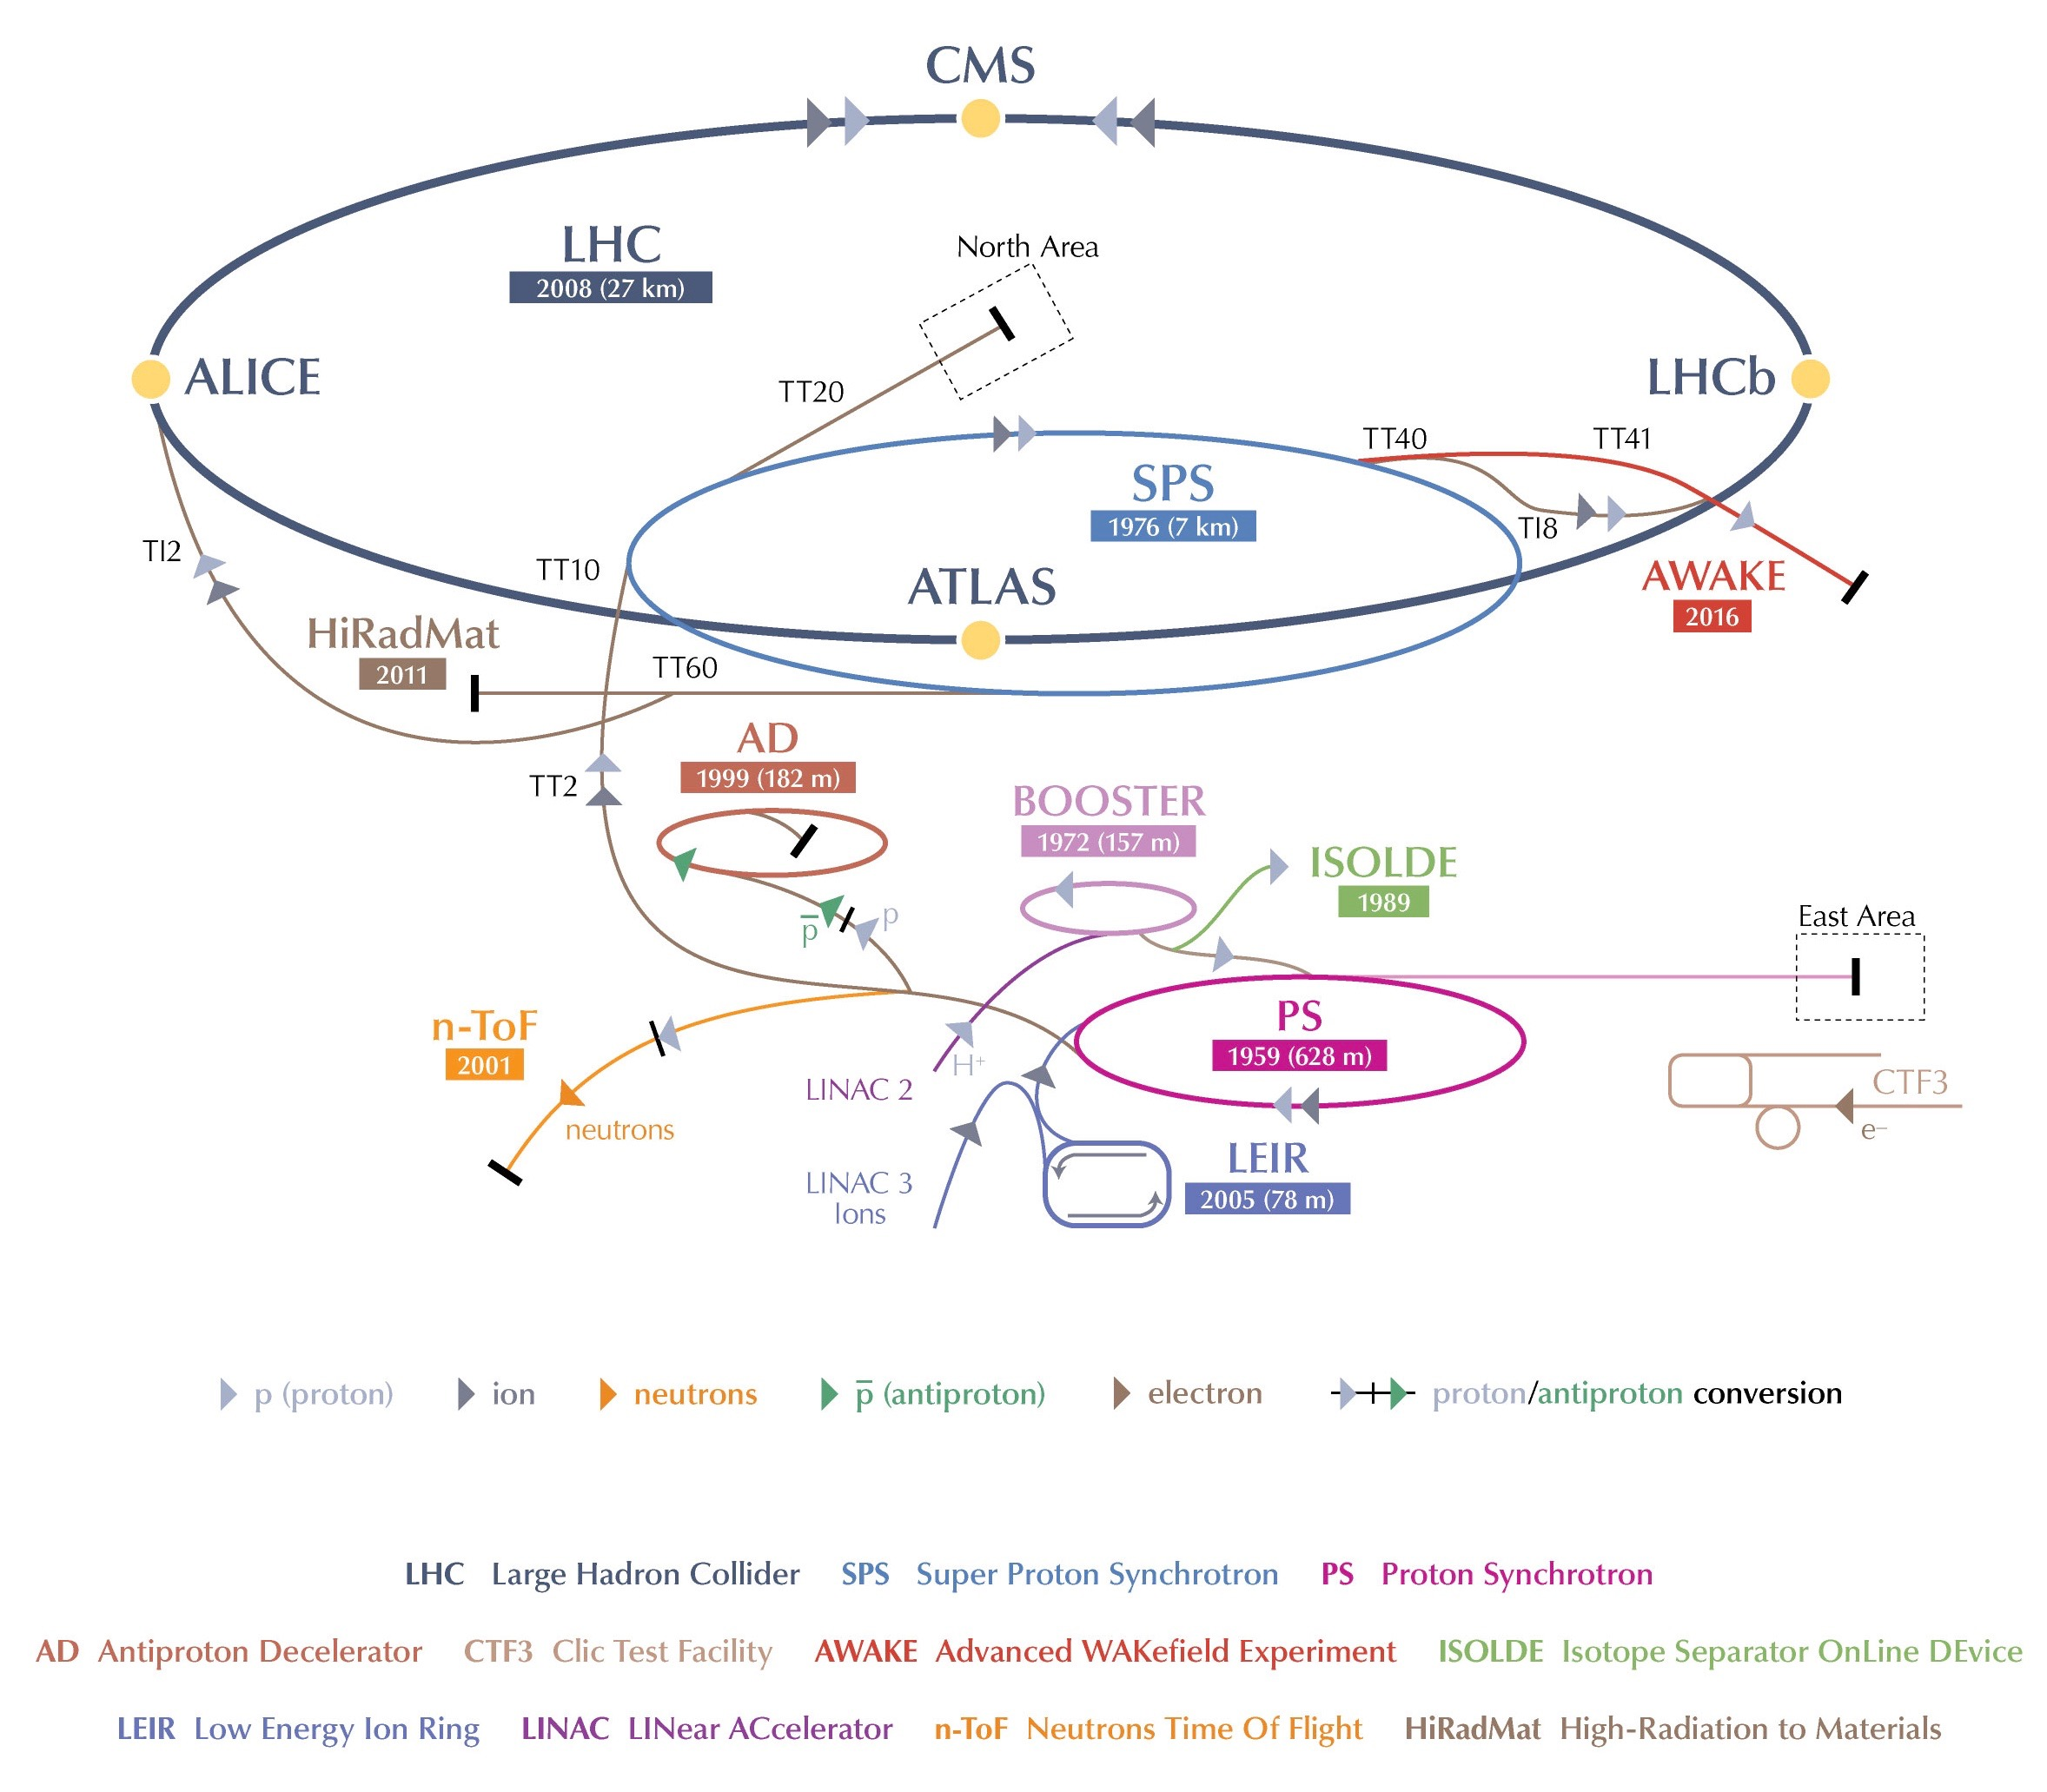
\includegraphics[width=1.0\textwidth]{./Figs/LHC_LHCb/accelerator_complex.jpg}
  \caption{The accelerator complex at CERN. The chain of accelerators used to provide protons to the LHC begins with the Linac 2 which accelerates protons to 50~\mev, the protons are passed to the Proton Synchrotron Booster that accelerates them to 1.4 \gev. The Proton Synchrotron is next in the chain, accelerating protons to 25~\gev and creating the desired spacing between proton bunches. Then finally the Super Proton Synchrotron accelerates protons to 450~\gev ready for injection into the LHC. Source: CERN.}
  \label{fig:accelerator_chain}
\end{figure}



%The protons leave the chain of accelerators with of energy of 450~\gev per proton and in bunches of \~$10^{11}$ protons, as the bunches are injected into the LHC they are split into two oppositely circulating beams.
%The LHC accelerates the protons to the desired centre-of-mass energy using supercooled radio frequency cavities and guides them around the ring with superconducting dipole magnets. %I could add here some details about the magnets and how the LHC accelerates the protons.
%Once the required energy has been reached, the bunches are focused using quadrupole magnets before being brought to collided at 4 interaction points around the LHC ring.% at a bunch crossing rate of 40~MHz. 

The centre-of-mass energy of a collider is an important measure of its performance as it describes the energy available to create particles during $pp$ collisions. Another important measure of collider performance is the instantaneous luminosity a collider can provide. The instantaneous luminosity, $\mathcal{L}$, is a measure of how many collisions occur per second, and is given by
\begin{equation}
\mathcal{L} = \frac{N^{2} f n_{b}}{\mathcal{F}},
\label{eq:inst_lumi}
\end{equation}
where $N$ is the number of protons per bunch, $n_{b}$ the number of bunches per beam, $f$ the bunch revolution frequency and $\mathcal{F}$ contains information about the beam geometry. The LHC is designed to operate at a maximum instantaneous luminosity of $10^{34}$~cm$^{-2}$s$^{-1}$. To reach this luminosity the LHC can have up to 2808 proton bunches per beam with a revolution frequency of 11.245 kHz and a separation of 25 ns between each proton bunch. %, therefore the separation between proton bunches can be as short as 25~ns. 
The higher the luminosity, the more collisions happen in a second and the more particles can be produced, this is either advantageous or disadvantageous depending on the particle interactions that are being studied.
% and the detector design that records the collisions. 
Therefore the luminosity delivered at each interaction point can be tuned using the quadrupole magnets by altering the shape and the orbit of each bunch to suit the experiments at each interaction point.



There are seven experiments around the LHC that study particles produced in proton and heavy ion collisions at the interaction points. These detectors are: %. The main physics goals of these experiments are desribed briefly in the following:
\begin{itemize}
\item ATLAS~\cite{Aad:2008zzm} and CMS~\cite{Chatrchyan:2008aa}, are general purpose detectors designed to search for the Higgs boson and NP effects that are beyond the scope of the SM. These experiments operate at the full instantaneous luminosity of the LHC; %Perhaps say we found the Higgs?
\item ALICE~\cite{Aamodt:2008zz} studies quark-gluon plasma produced in heavy ion collisions to understand conditions similar to those present in the early universe, products from $pp$ and lead-proton collisions are used to understand collisions of lead ions;
\item  TOTEM~\cite{Anelli:2008zza} studies properties of protons as they collide head on at the LHC, to measure the $pp$ interaction cross section and understand the internal structure of protons; %luminosity% a and the 
\item MOEDAL~\cite{Pinfold:2009oia} is designed to detect magnetic monopoles and massive stable charged particles predicted by theories that go beyond the scope of the SM;
\item the LHCf experiment~\cite{Adriani:2008zz} studies particles that are created at very small angles to the incident proton beams to understand similar processes that occur in cosmic rays; and %Finally there is the Large Hadron Collider Beauty experiment (LHCb) that will be described in the next section. %, this experiment was designed to studies rare $b$-hadron decays and $\mathcal{CP}$ violating processes and operates at a lower luminosity and has a smaller angular acceptance than the general purpose detectors. %Should probably include the full experiment names as I have done for LHCb or not include the name for LHCb.
\item the final experiment is the LHCb experiment~\cite{Alves:2008zz} is designed to study rare $b$-hadron decays and $\mathcal{CP}$ violating processes. It operates at a lower luminosity and has a smaller angular acceptance than the general purpose detectors. 
\end{itemize}
%Proton beams first circulated the LHC in 2008 and since then there have been two physics runs separated by a long shutdown period.

Proton beams first circulated the LHC in 2008 and since then the experiments have recorded data during two experiment runs separated by a long shutdown period.
The amount of data recorded by an experiment is given in terms of the time integrated luminosity.
Run 1 began in 2010 and continued until 2013, during this time protons were collided with a centre-of-mass energies of $\sqrt{s}$~=~7~and $\sqrt{s}$~=8~TeV. 
After Run~1 there was a period of long shut down during which work was done to prepare the LHC to operate at higher energies, renovation work was performed on the accelerators that provide the LHC with protons and the experiments were prepared for the second experiment run.
Run~2 began in 2015 with proton collisions at a centre-of-mass energy of $\sqrt{s}$~=~13~TeV, and will continue until 2018 when a second period of upgrades and maintenance will begin. The centre-of-mass energies for $pp$ collisions for each year of operation so far are summarised in Table~\ref{tab:Runs}, alongside the integrated luminosity recorded by the ATLAS, CMS and LHCb experiments. %for the experiments.

%https://twiki.cern.ch/twiki/bin/view/CMSPublic/LumiPublicResults#2010_Proton_Proton_Collisions
%https://twiki.cern.ch/twiki/bin/view/AtlasPublic/LuminosityPublicResultsRun2
%https://twiki.cern.ch/twiki/bin/view/AtlasPublic/LuminosityPublicResultsRun2
%http://lhcb-public.web.cern.ch/lhcb-public/
\begin{table}[t]
\begin{center}
\begin{tabular}{lccccc}
\toprule \toprule
\multirow{2}{*}{Run} & \multirow{2}{*}{Year} & \multirow{2}{*}{$\sqrt{s}$ / \tev} & \multicolumn{3}{c}{Integrated luminosity / \fb}\\ 
\cmidrule{4-6}
    &     &                             & ATLAS &  CMS       & LHCb \\ \midrule
 \multirow{3}{*}{Run 1}    & 2010 & 7   & 0.04  & 0.04        & 0.04\\
     & 2011 & 7                         & 5.08  & 5.55      &  1.11 \\
    & 2012 & 8                          & 21.3  & 21.79  &  2.08 \\ 
\midrule
\multirow{2}{*}{Run 2}    & 2015 & 13   & 3.9   & 3.81         & 0.32\\
    & 2016 & 13                         & 35.6  & 37.76         & 1.67     \\ \bottomrule \bottomrule

\end{tabular}
\vspace{0.7cm}
\caption{Centre-of-mass energy for each year of data taking and the integrated luminosity recorded by ATLAS, CMS and LHCb during $pp$ collisions~\cite{LHCblumi,CMSlumi,ALTASlumi}.}
\label{tab:Runs}
\end{center}
\vspace{-1.0cm}
\end{table}




\section{The LHCb experiment}
\label{LHCb}
The LHCb experiment was built to study the SM and search for NP phenomena through the study of $\mathcal{CP}$-violating decays and rare $b$-hadron decays. 
%The LHCb experiment was built to study CP violation and rare decays of \bhadrons to search for new physics processes that could be revealed in these decays. 
At the LHC the dominant production mechanisms of \bbbar pairs are gluon-gluon fusion, quark anti-quark annihilation and gluon-gluon splitting, as shown in Figure~\ref{fig:bbbarprod}. The \bbbar pairs produced travel at small angles relative to the beam pipe and the angular distribution is shown in Figure~\ref{fig:bbar_production}. % and hadronize to form a range of \bhadrons, including $B^{+}$, $B^{0}_{s}$ and $\Lambda^{0}_{b}$, that are studied by LHCb. 
The $b\bar{b}$ pair is created at the primary vertex of an event, where the protons collide. The quarks then hadronise to form a range of \bhadrons, including $B^{+}$, $B^{0}_{s}$ and $\Lambda^{0}_{b}$. % a $b$ hadron. 
A typical $b$ hadron will exist for approximately 1.5 ps~\cite{Olive:2016xmw} before decaying into leptons, light hadrons or a mixture of both. The vertex where the $b$-hadron decays is know as the secondary vertex and is displaced by a few centimetres from the primary vertex. %The LHCb experiment was built to optimsed cost and physics output in the study of these decays. 
The LHCb experiment was designed considering both the cost of the detector and the physics processes that could be studied with it. 



\begin{figure}[tbp]
  \centering
  \begin{subfigure}[b]{0.4\textwidth}
    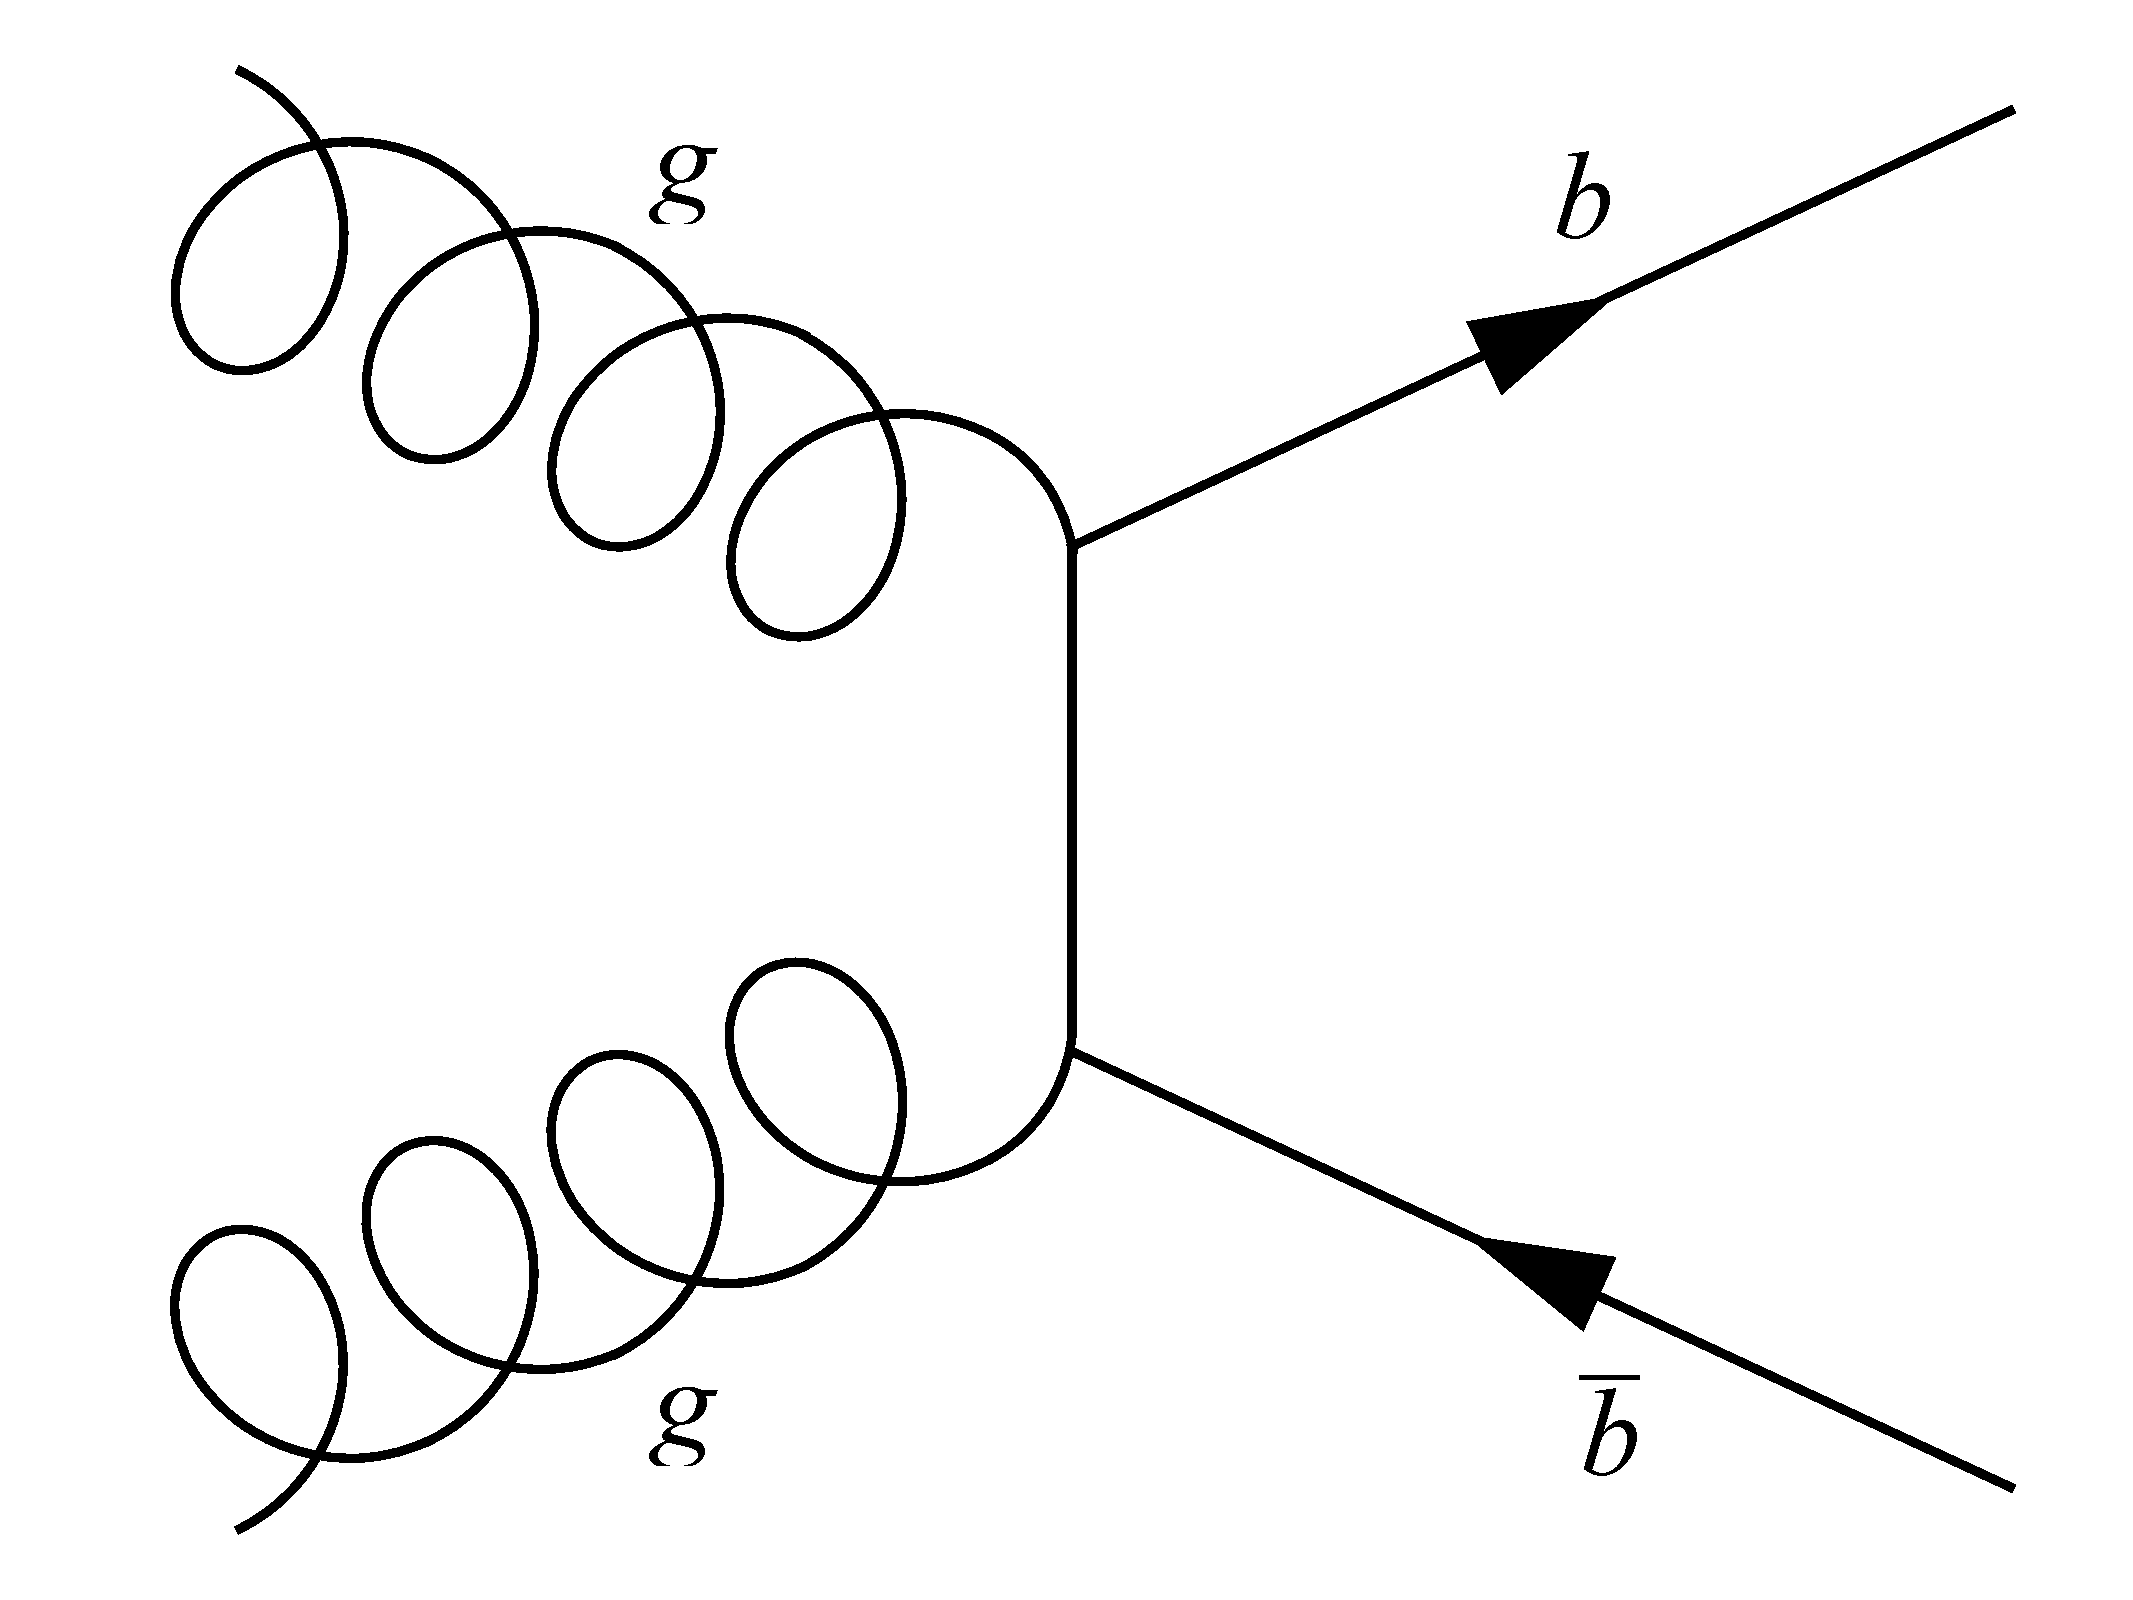
\includegraphics[width=\textwidth]{./Figs/LHC_LHCb/bbbar_prod_1.pdf}
    \caption{}
    \label{fig:}   
  \end{subfigure}             
  \begin{subfigure}[b]{0.4\textwidth}
    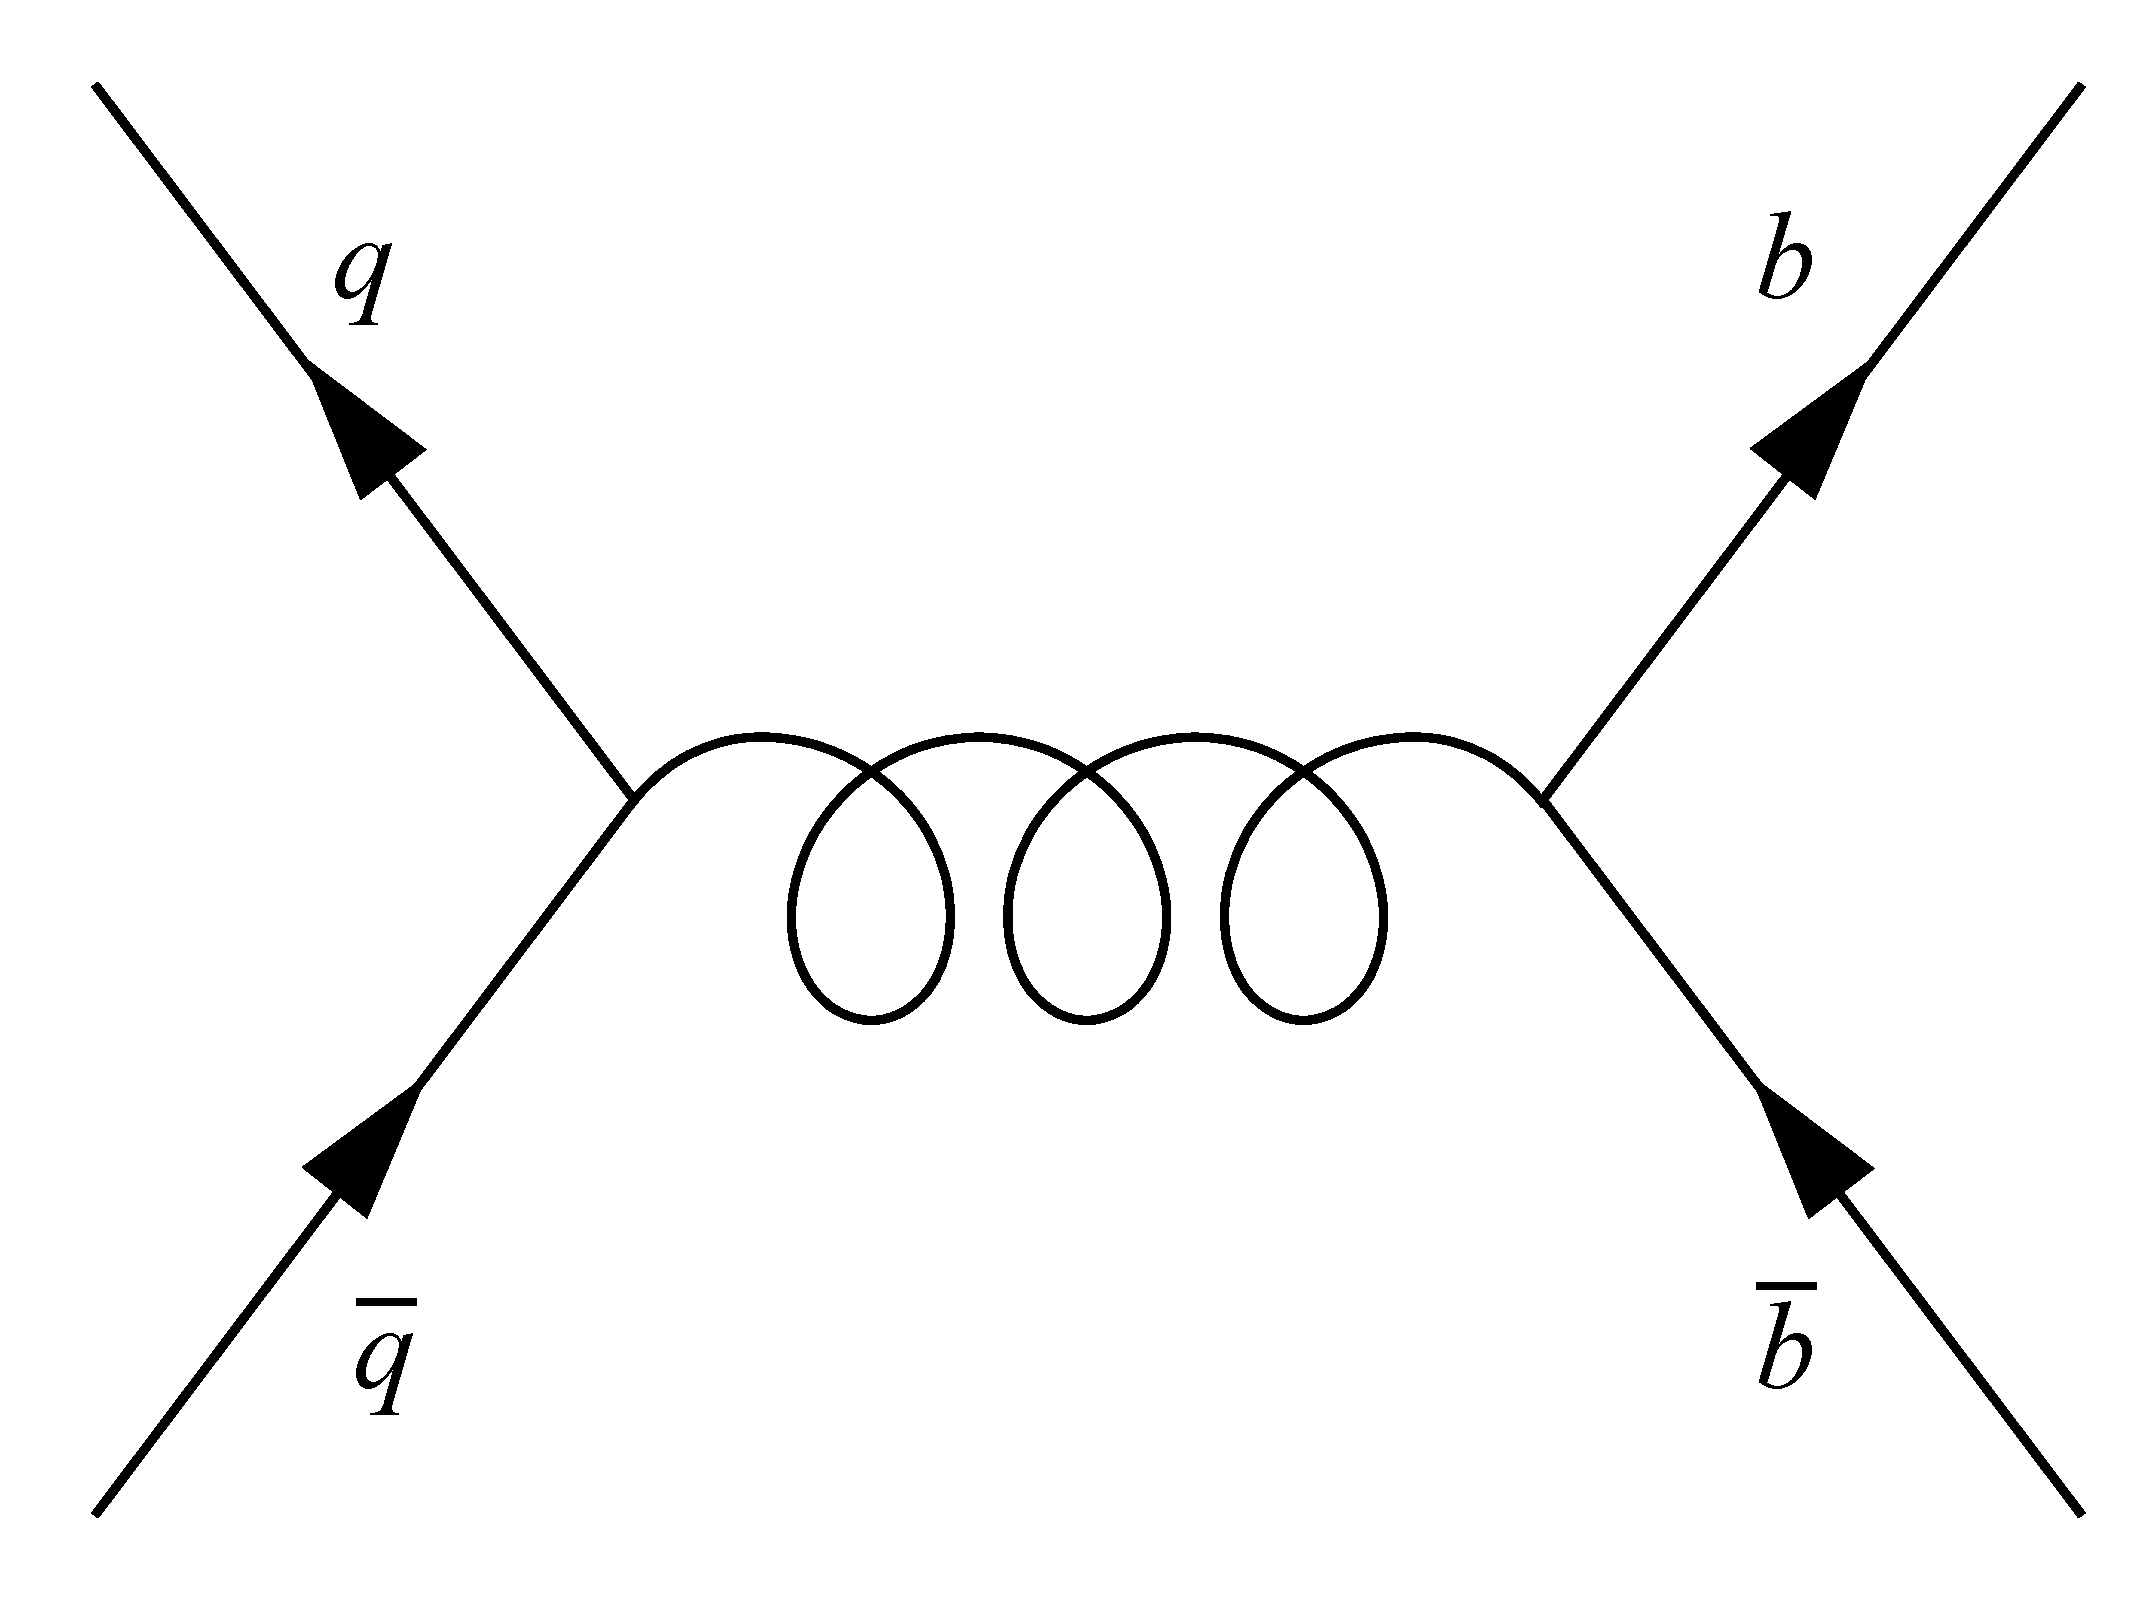
\includegraphics[width=\textwidth]{./Figs/LHC_LHCb/bbbar_prod_2.pdf}
    \caption{}
    \label{fig:}
  \end{subfigure}             
  \begin{subfigure}[b]{0.4\textwidth}
    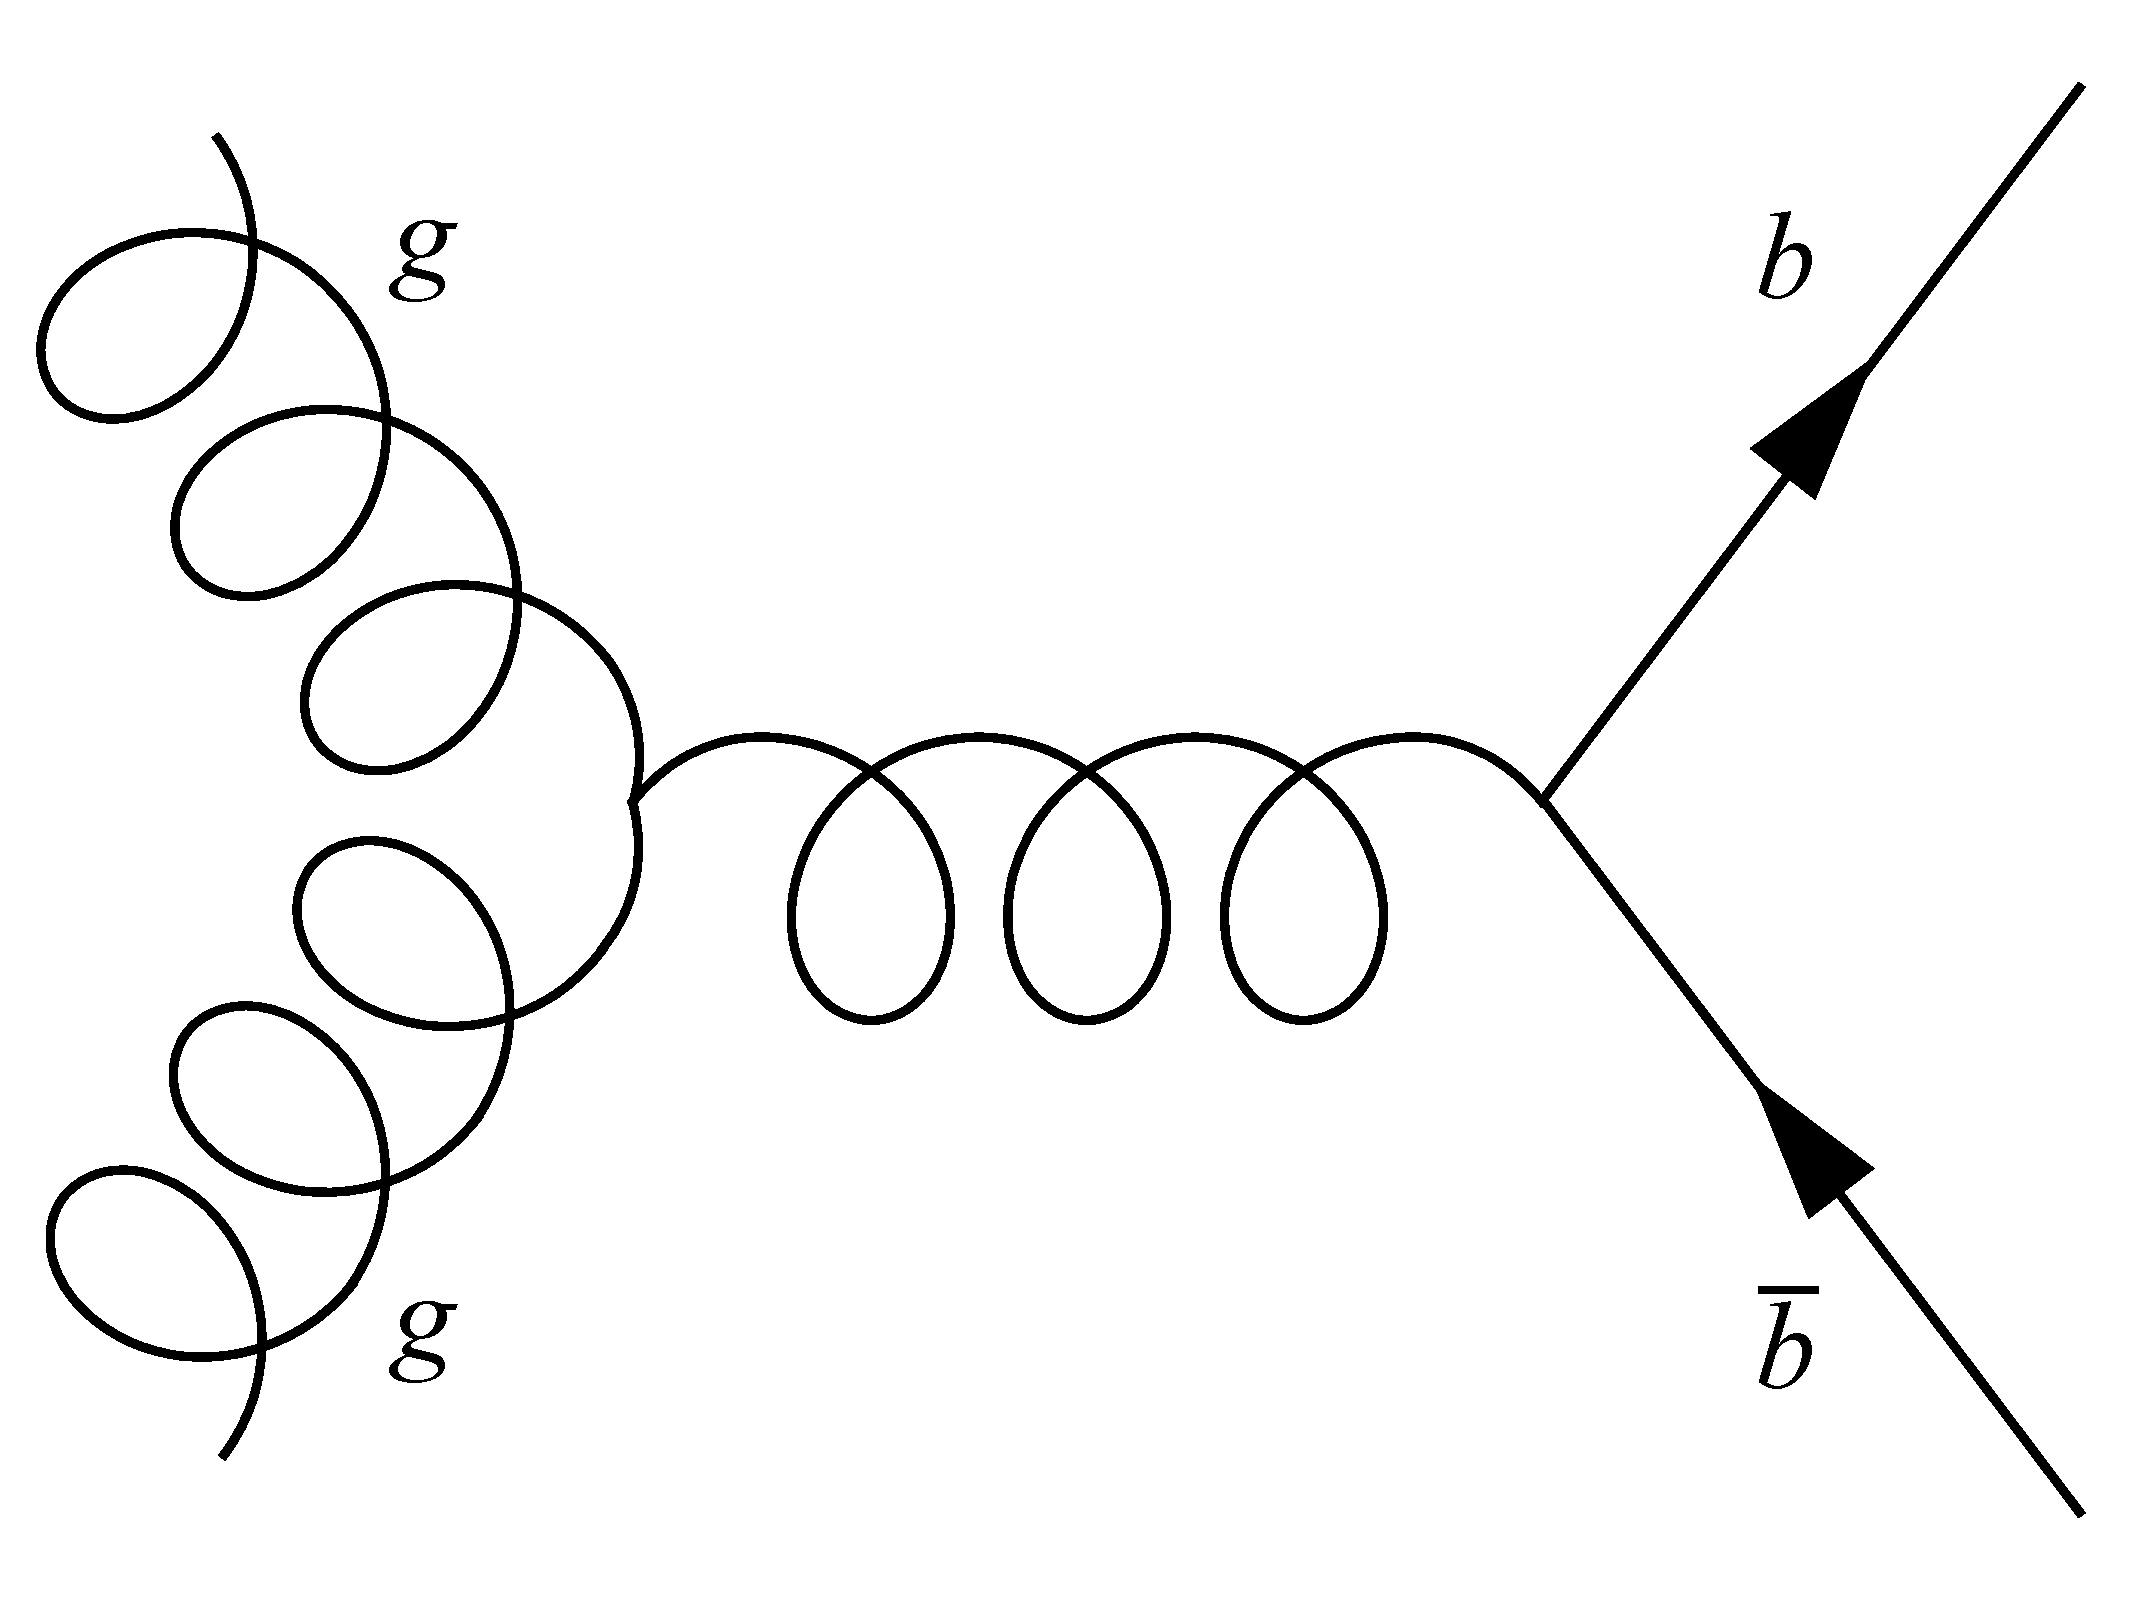
\includegraphics[width=\textwidth]{./Figs/LHC_LHCb/bbbar_prod_3.pdf}
    \caption{}
    \label{fig:}
  \end{subfigure}
  \caption{Dominant production mechanisms for \bbbar pairs created in $pp$ collisions are: gluon-gluon fusion (a); quark anti-quark annihilation (b); and gluon-gluon splitting (c).}
  \label{fig:bbbarprod}
\end{figure}

\begin{figure}[ptb] 
  \centering    
  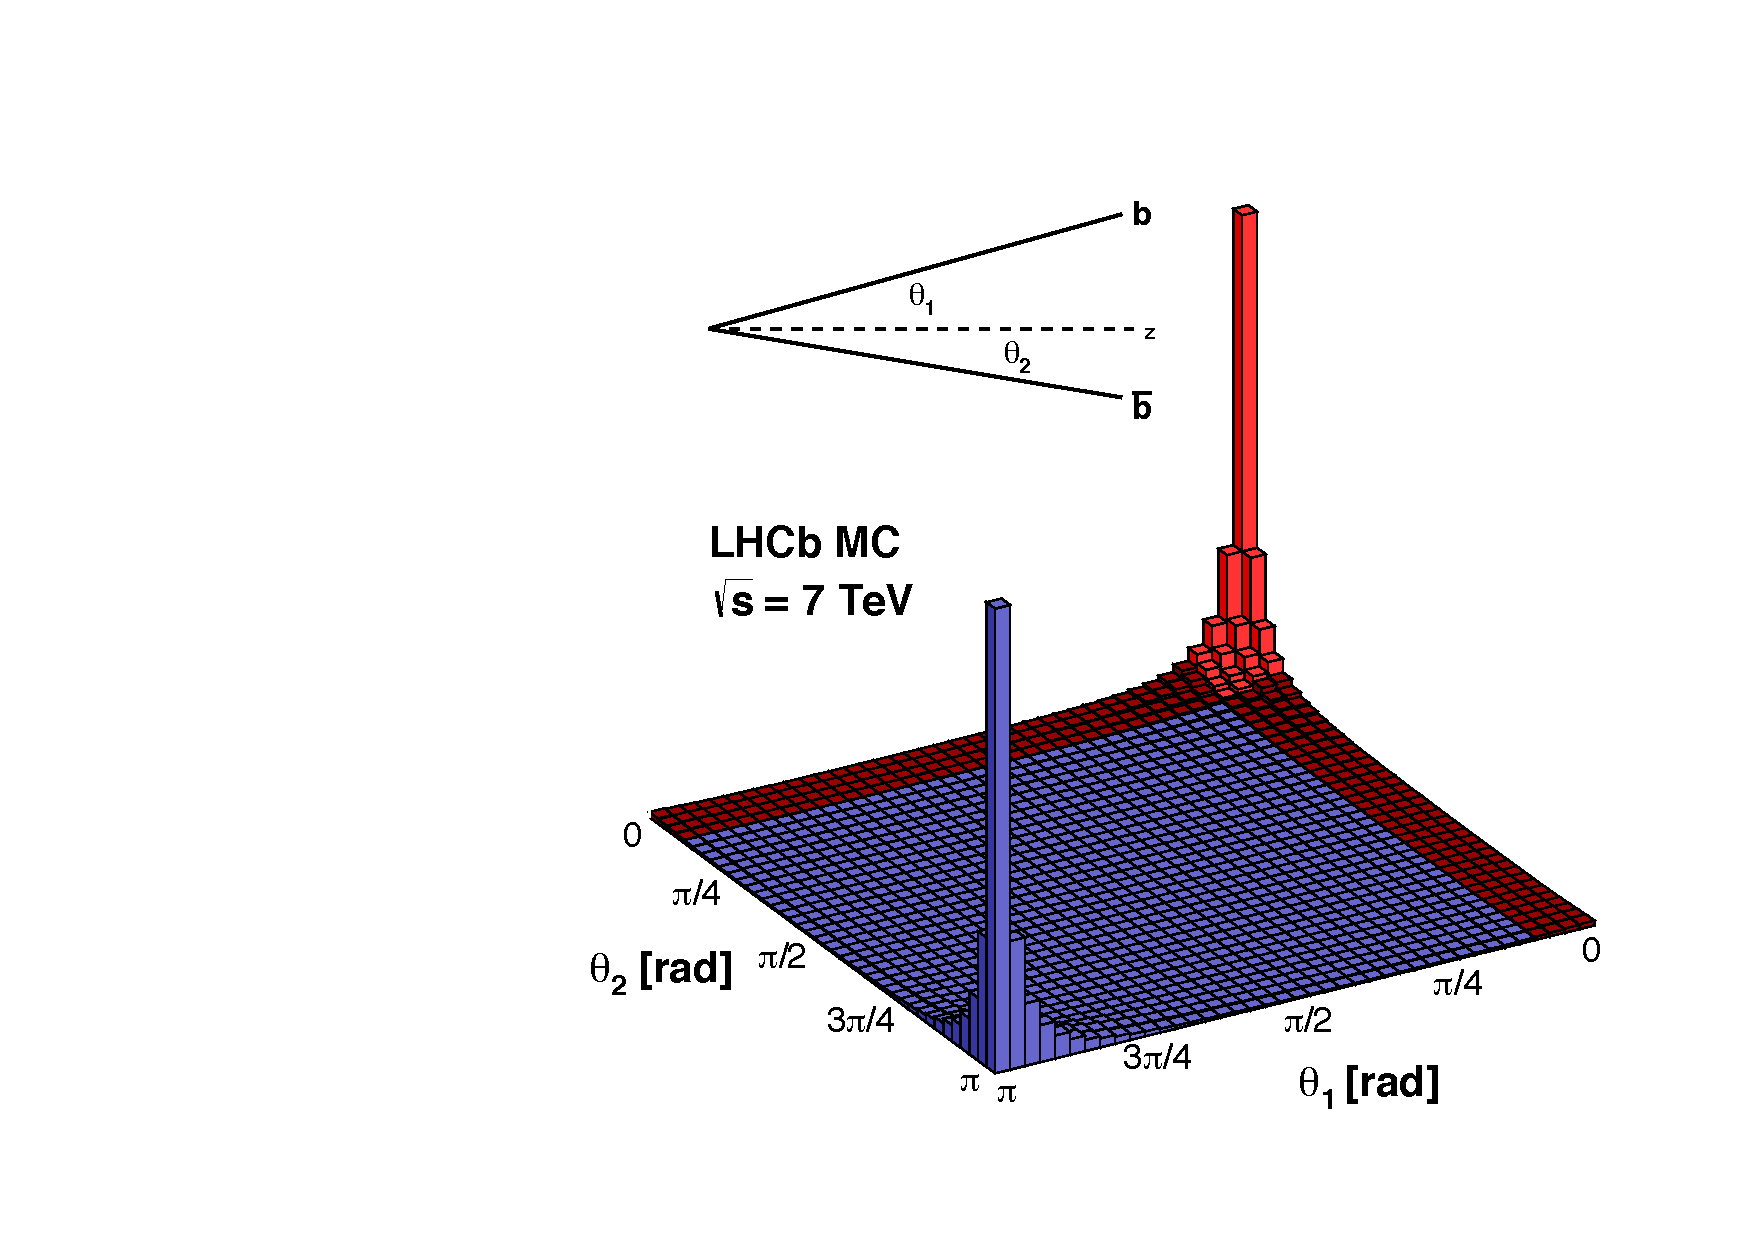
\includegraphics[ width=0.65\textwidth]{./Figs/LHC_LHCb/07_rad_acc_scheme_right.pdf}%b_distrib_lhcb.pdf}
  \caption{Simulated angular distribution for \bbbar production at the LHC at center-of-mass energies of 7~\tev, angles are relative to the beam pipe with $\theta =0$ in the forward direction and $\theta = \pi$ in the backward direction. The red area shows \bbbar pairs that are produced within the angular coverage of the LHCb detector and the purple shaded area shows \bbbar pairs outside the detector coverage. Source: LHCb.}
 \label{fig:bbar_production}
\end{figure}


%\begin{figure}[tbp]
%  \centering
%  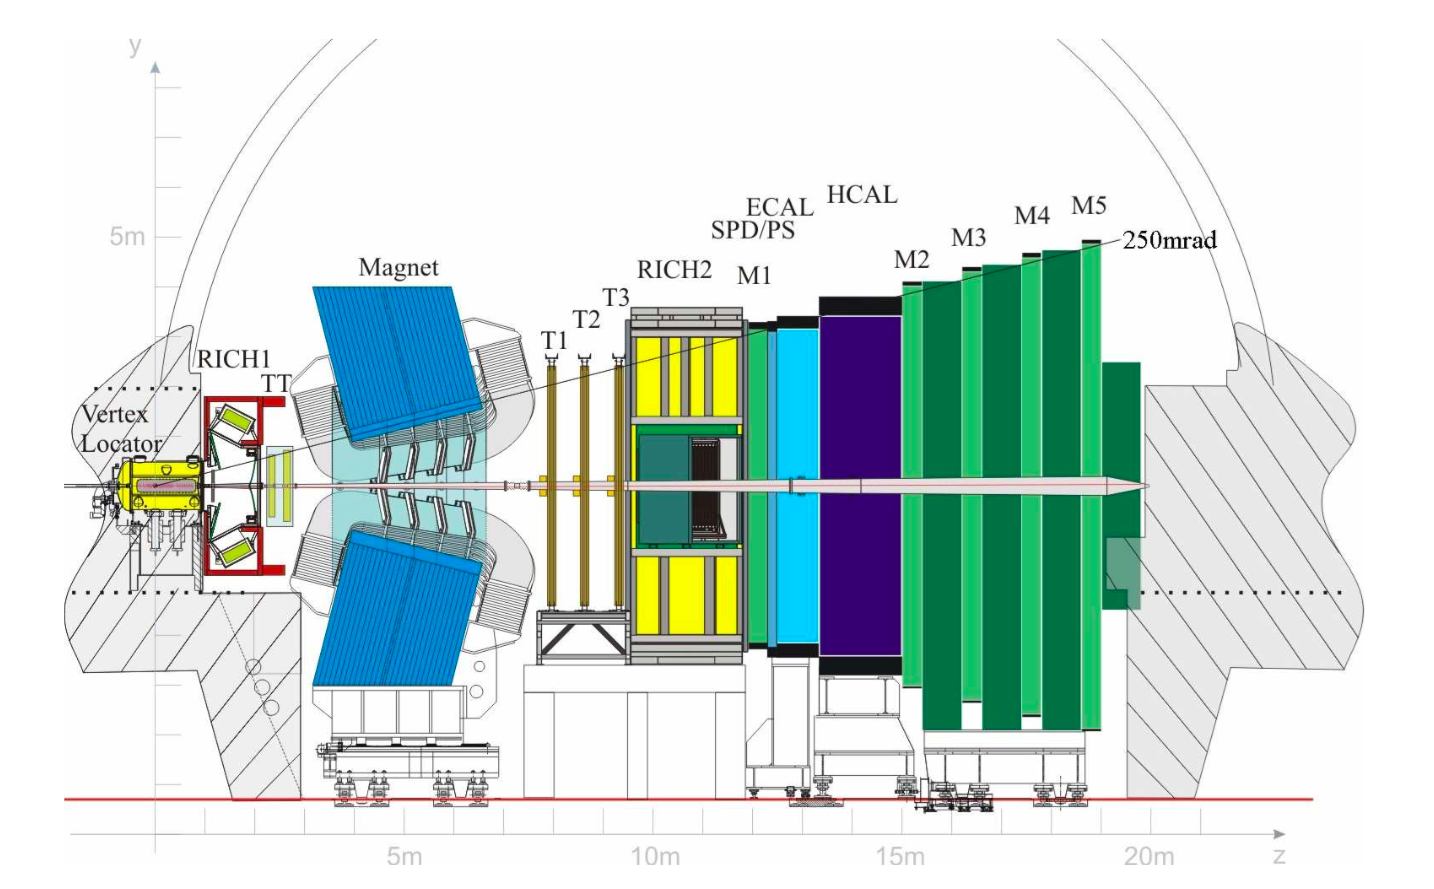
\includegraphics[ width=1.0\textwidth]{./Figs/LHC_LHCb/lhcb.png}
%  \caption{Cross section .}
%  \label{fig:bbbarprod}
%\end{figure}

The LHCb experiment is a single arm forward spectrometer, with an angular coverage of 10 to 300~mrad in the vertical direction and 10 to 250~mrad in the horizontal direction relative to the beam pipe. %The angular coverage includes most b paris in one directs  sdfhjgajkfhdfsjfgf  was chosen to exploit the small angles at which \bbbar pairs are produced. 
A cross-section of the LHCb detector is shown in Figure \ref{fig:LHCb_detector}, where a right-handed coordinate system is used. The $z$ and $y$ directions are shown in in the figure and the $x$-axis points into the page. Protons collide at the interaction point on the left-hand side of the diagram, a subset of particles produced during the collisions travel through the detector leaving information in the sub-detectors. The coordinate system is chosen so that the interaction point is approximately at $x = y= z = 0$. %Most particles produced in the $pp$ collisions do not fall in the angular coverage of the LHCb experiment however
The information deposited in the sub-detectors is reconstructed to determine what happened during the $pp$ collisions. %
Although the angular coverage of the LHCb experiment is only 4\% of the total solid angle, it covers the smaller angles relative to the beam pipe at which \bbbar pairs are produced, as illustrated by the red shaded area in Figure~\ref{fig:bbar_production}.
%The information deposited in the sub-detectors is reconstructed to determine what happened during the $pp$ collisions. %The angular coverage of the detector is such that appromixately half of the $b\bar{b}$ pairs created in the collisions will travel through the detector. 

\begin{figure}[tbp] 
  \centering    
  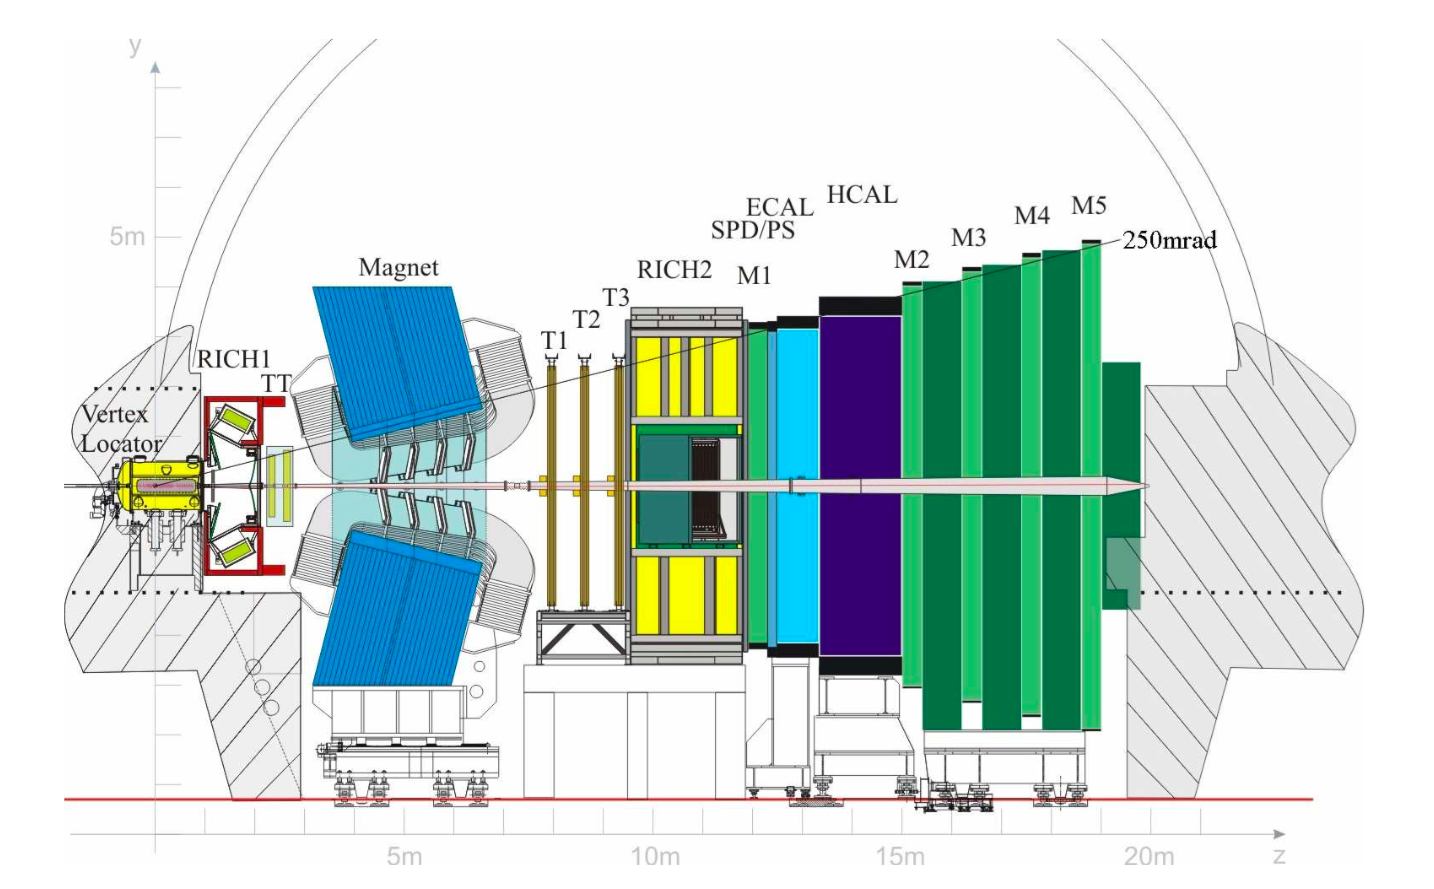
\includegraphics[ width=1.0\textwidth]{./Figs/LHC_LHCb/lhcb.png}
  \caption{Schematic of the LHCb detector \cite{Alves:2008zz}. A right-handed coordinate system is chosen where the $x$ and $z$ directions are shown and the $x$ direct points into the page.}
  \label{fig:LHCb_detector}
\end{figure}


The different sub-detectors have been chosen to exploit the characteristics of \bhadron decays and fall into two distinct categories; tracking detectors and particle identification detectors. The sub-detectors and their performances are described briefly in the following sections along with the trigger system and software needed to analyse the data collected by the experiment. %Finally the data recorded by the experiment during Run 1 and Run 2 is presented in Section \ref{LHCb_data}. 
For a more detailed description of the detector and its performance during Run 1, see references~\cite{TDR1,Alves:2008zz,LHCb:2003ab,Aaij:2014jba} and those given in the text.




\subsection{Tracking}
\label{Tracking}

The tracking system within the LHCb experiment consists of the vertex locator, a dipole magnet and three tracking stations after the magnet. The vertex locator and tracking stations are described in Sections~\ref{VELO} and ~\ref{Tracking_Stations} and the magnet is described in Section~\ref{Magnet}. Together, the sub-detectors provide precise information on the passage of charged particles through the detector, a measurement of the particle momentum and electric charge. 
The tracking detectors work on the principle that the passage of high energy charged particles through silicon or ionised gas causes the excitation or ionisation of atoms in the material. The release of this energy is recorded and translated into an electrical signal that reveals the path of a particle. 
%Precise particle track and momentum measurements are necessary to obtain the accurate particle mass and decay time measurements that help distinguish between different hadrons decaying in the LHCb detector. 
Hits left in the different detectors are combined to form tracks that are used to identify particle decays as described in Section~\ref{sec:Track_recon}.
\subsubsection{The vertex locator}
\label{VELO}
The VErtex LOcator (VELO)~\cite{Barbosa-Marinho:504321, LHCbVELOGroup:2014uea} is a silicon detector surrounding the interaction point. Its main purpose is to provide precise information about the $pp$ interaction vertices and secondary decay vertices of the particles produced. Information from the VELO enables precise measurements of particle lifetimes and the impact parameters of particle tracks necessary for the study of particle decays. % physics analyses.


The VELO is made of two identical halves, each half consists of 21 stations containing two silicon sensors arranged along the beam pipe. The two halves of the VELO slot together and there is a small gap in the centre for the beams to pass through. The arrangement of sensors along the $z$-axis, shown in Figure \ref{fig:velo}, is designed so that the sensors cover the full LHCb acceptance and a charged particle within the detector acceptance will pass through at least three stations. 

Each station is composed of two sensors: the R-sensor that measures the radial distance of charged particles from the beam axis; and the $\phi$-sensor that measures the azimuthal angle of the particle with respect to the $z$-axis of the detector as shown in Figure~\ref{fig:LHCb_detector}. The information from the sensors is combined with the distance of sensors along the $z$-axis is used to reconstruct charged particle trajectories.
The cylindrical geometry used for the VELO sensors, shown in Figure~\ref{fig:velo_sensor}, is chosen to allow fast reconstruction of particle trajectories in the VELO.
%In each station the two sensors measure different coordinates, one measures the $r$ coordinates of charged particles and the other measures the $\phi$ coordinates as shown in Figure~\ref{fig:velo_sensor}. The $r$, $\phi$ coordinates and the $z$ placement of the sensors are used to reconstruct charged particle trajectories. Cylindrical coordinates were chosen to allow fast reconstruction of particle trajectories in the VELO.

\begin{figure}[tbp] 
  \centering    
  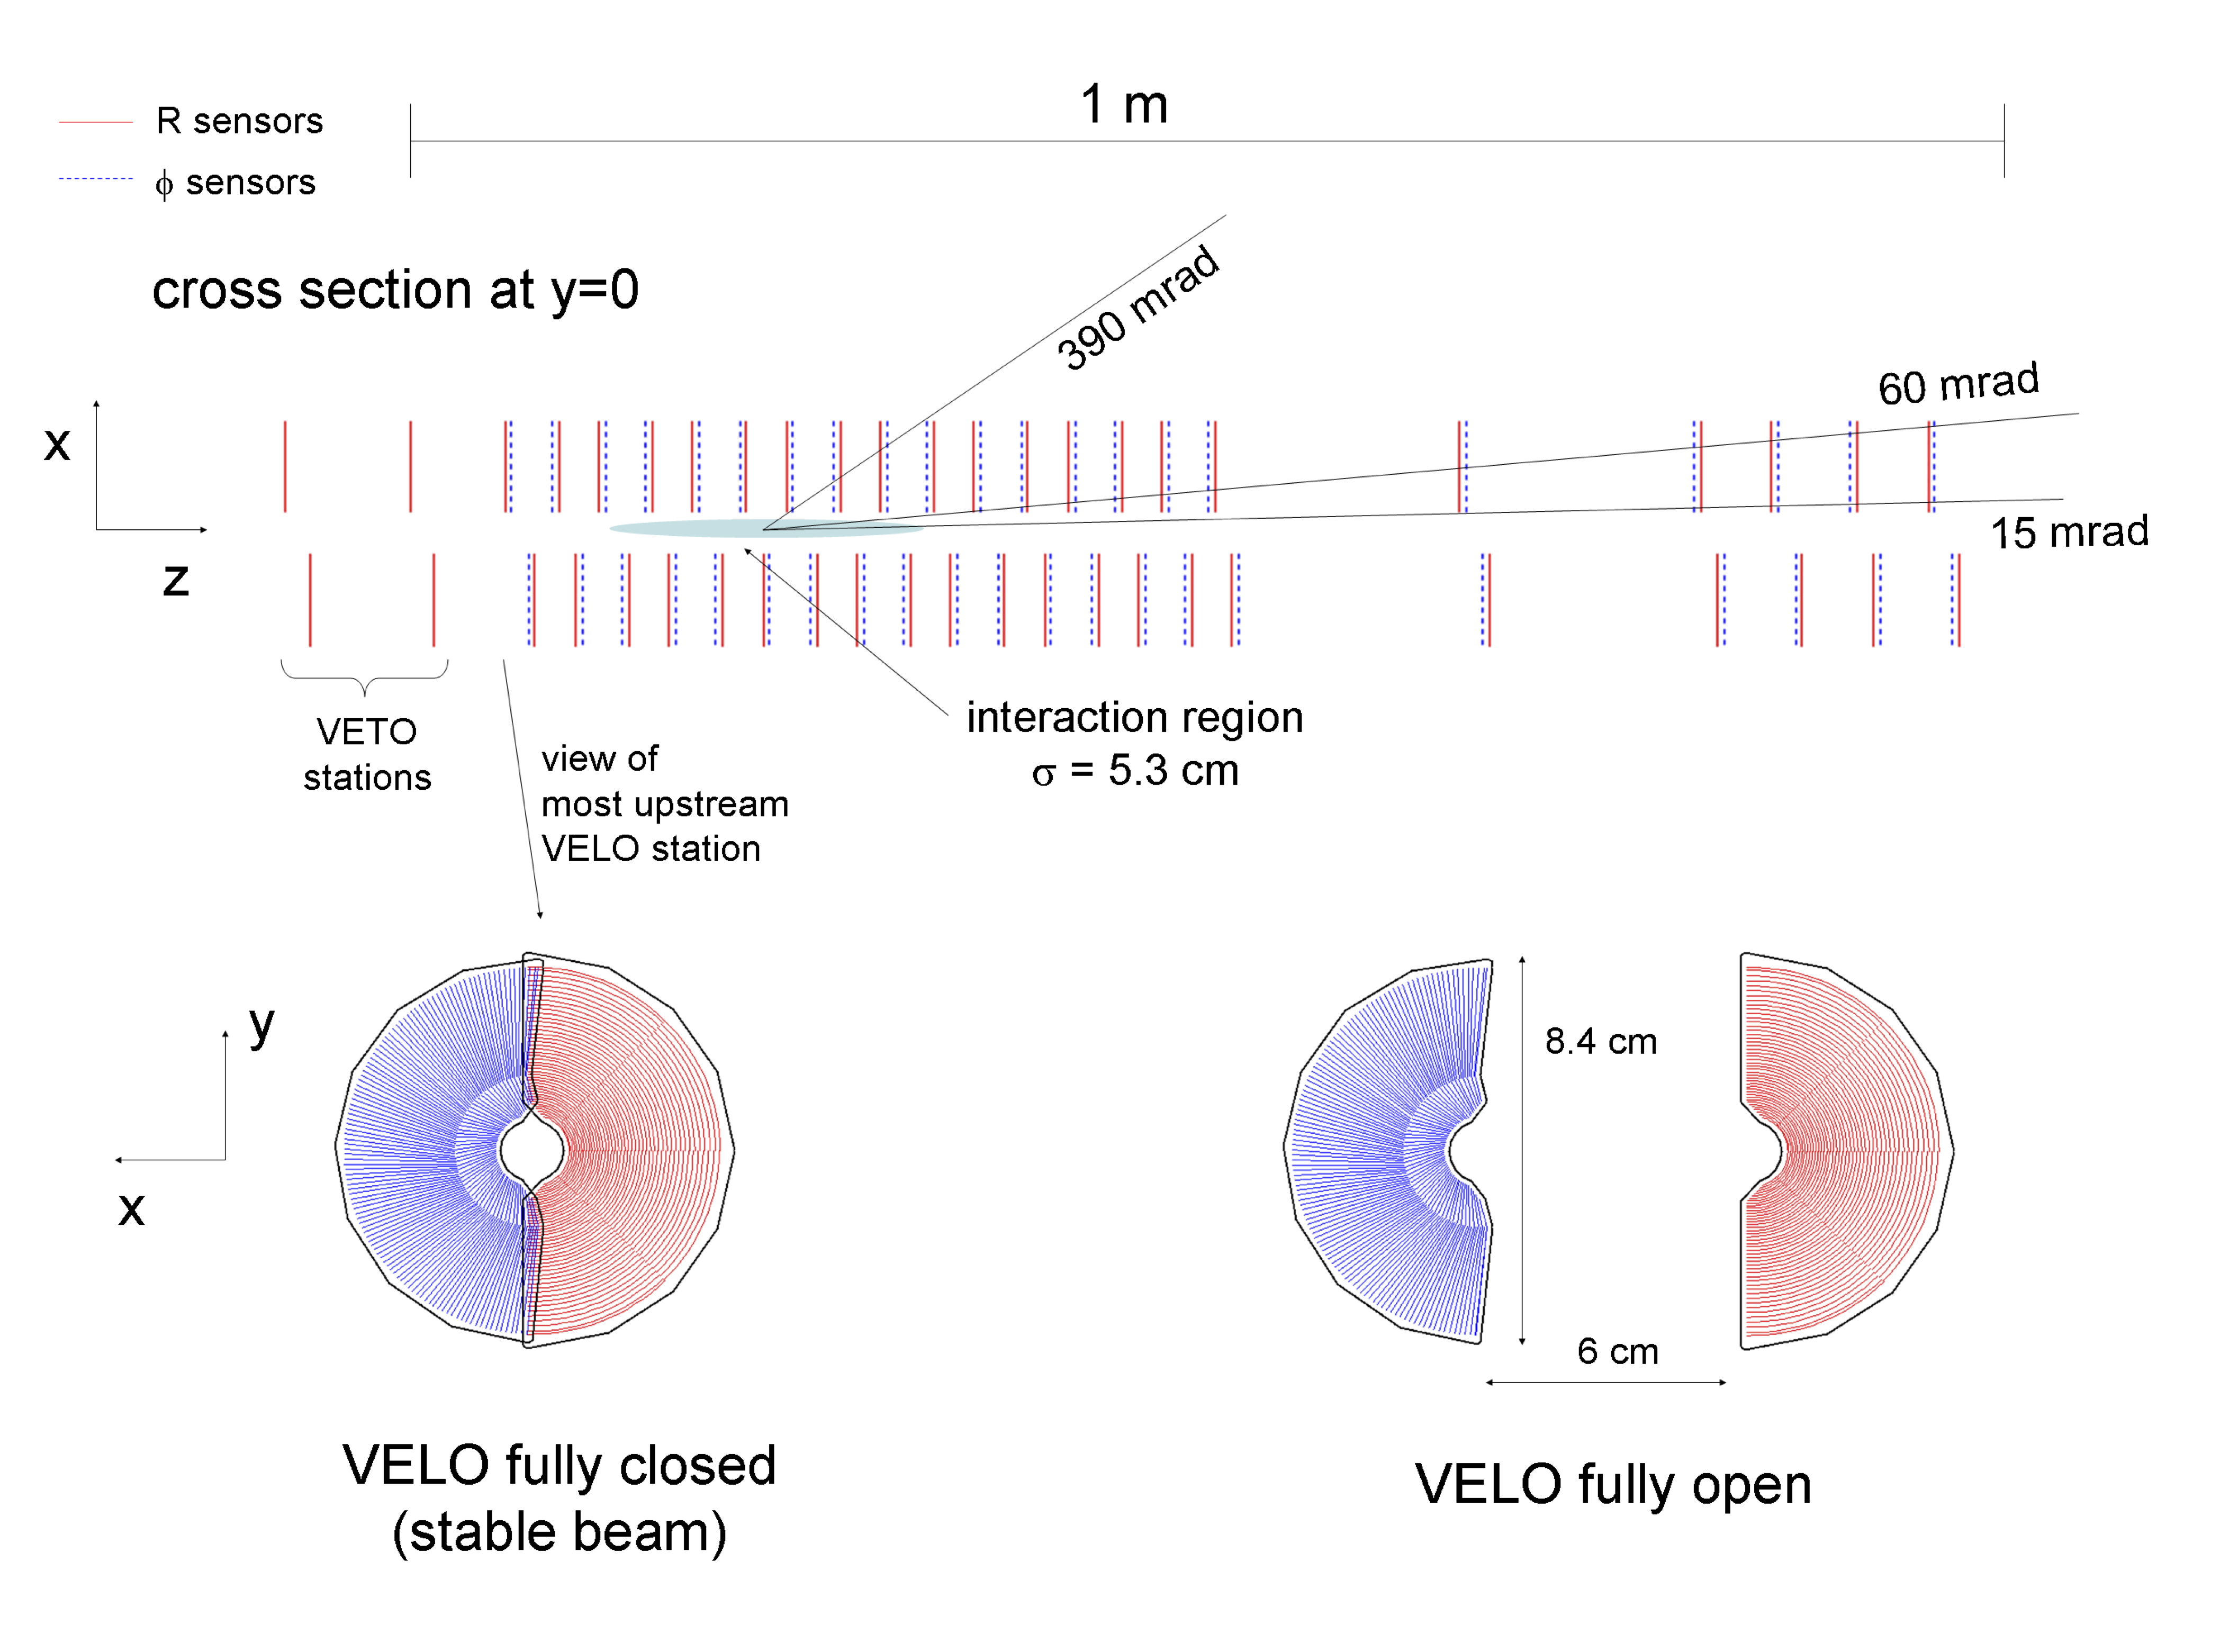
\includegraphics[ width=0.7\textwidth]{./Figs/LHC_LHCb/velo.png}
  \caption{The VELO layout and position of sensors along the beam axis \cite{Alves:2008zz}.}
  \label{fig:velo}
\end{figure}


\begin{figure}[tbp]
  \centering
  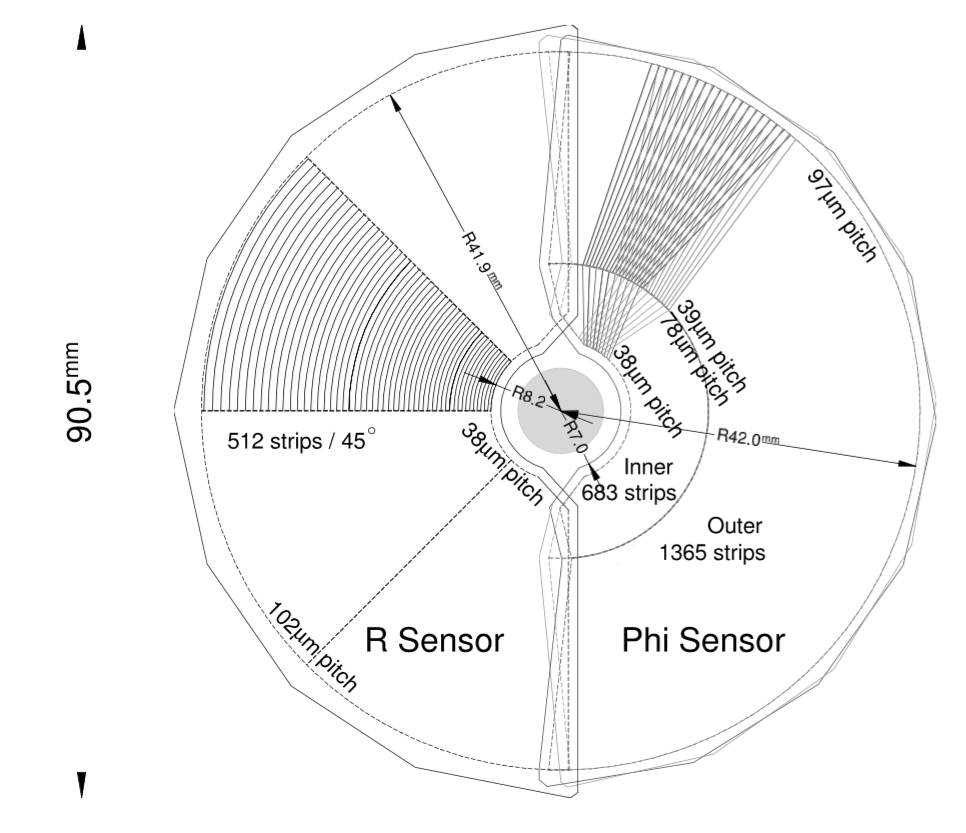
\includegraphics[ width=0.6\textwidth]{./Figs/LHC_LHCb/Velo_sensor_diagram.png}
  \caption{Diagram of $r$ and $\phi$ sensor layouts~\cite{Alves:2008zz}.}
  \label{fig:velo_sensor}
\end{figure}


The momentum resolution achievable for charged tracks by the LHCb experiment is limited by the multiple scattering of particles as they travel through material the detector is made from. Therefore, to ensure good momentum resolution throughout the detector, the VELO is kept in a vacuum to reduce the material each particle must travel through. %its material budget. 
Each half of the VELO is enclosed inside an aluminium box, which keeps it in a vacuum and shields the electronic readouts from radio frequencies generated by the beam. %The overall material budget of the VELO comes to 17.5 $\%$ of a radiation length.

Excellent resolution of the position of each vertex is required in the VELO to identify the particle decays that occur. To achieve this the sensors need to be as close as possible to the interaction point. This is achieved by making the VELO out of two retractable halves and including the $pp$ interaction point within the coverage of the VELO. 
%The sensors of the VELO are located as close as possible to the $pp$ interaction point in order to acheive excellent vertex resolution. The VELO is made out of retractable halves and including the interaction point within the coverage of the VELO. 
During data taking, when the VELO is recording particle tracks, the inner most part of the sensors are 8~mm from the beam axis. However, during the injection phase the width of the beam is much larger than 8~mm, therefore the halves of the VELO are retracted to 3~cm from the nominal beam axis. This keeps the VELO safe from unnecessary radiation damage. The two halves of the VELO are displaced by 150~mm in the $z$-direction, as shown in Figure~\ref{fig:velo}, so that when the VELO is closed, the sensors in each half overlap to help with detector alignment and reduced edge effects. 

%\begin{figure}[htb] 
%  \centering    
%  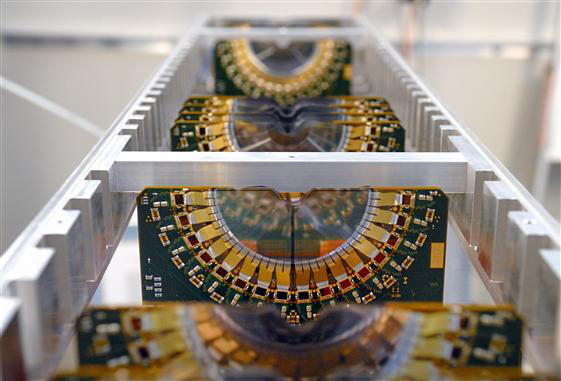
\includegraphics[ width=0.7\textwidth]{./Figs/LHC_LHCb/Velo_photo.jpg}% ./Figs/Detector/Velo_photo.jpg}
%  \caption{The velo Soure: LHCb.}
%  \label{fig:velo_photo}
%\end{figure}


%An additional purpose of the VELO is to act as a veto for high pile up events. There are 2 VELO sensors upstream of the interaction point that provide information to the trigger about how many $pp$ interactions there were with each bunch crossing. Events with large numbers of primary vertices are difficult and time consuming to reconstruct and lead to less precise measurements of particle decay properties. Information from the VELO is used to reject events with high numbers of primary vertices to ensure the best used of information from the detector.
An additional purpose of the VELO is to identify high pile-up events. There are two VELO sensors upstream of the interaction point that provide information to the trigger about how many $pp$ interactions there were in a bunch crossing. This information can be used to identify events with high numbers of primary vertices. %Events with large numbers of primary vertices are difficult and time consuming to reconstruct and lead to less precise measurements of particle decay properties. 
%Information from the VELO can used to reject events with high numbers of primary vertices to ensure the best used of information from the detector.

The VELO achieves a resolution on the position of each vertex of 10 - 20~$\mu$m transverse to the $z$ direction and 50 - 100~$\mu$m along the $z$ direction, the resolution of each track depends on the number of tracks in each event as shown in Figure~\ref{fig:Velo_PV_resolution}. The VELO also gives measurements on the impact parameters of particles tracks; the impact parameter (IP) is the distance of closest approach between a particle track and the primary vertex. Figure \ref{fig:IP_res} shows the IP resolution for 2012 data; a track with transverse momentum of 1~GeV/c has an impact parameter resolution of 35~$\mu$m. 



%Can I just put the track resolution possible with the VELO?
\begin{figure}[tbp] 
  \centering    
  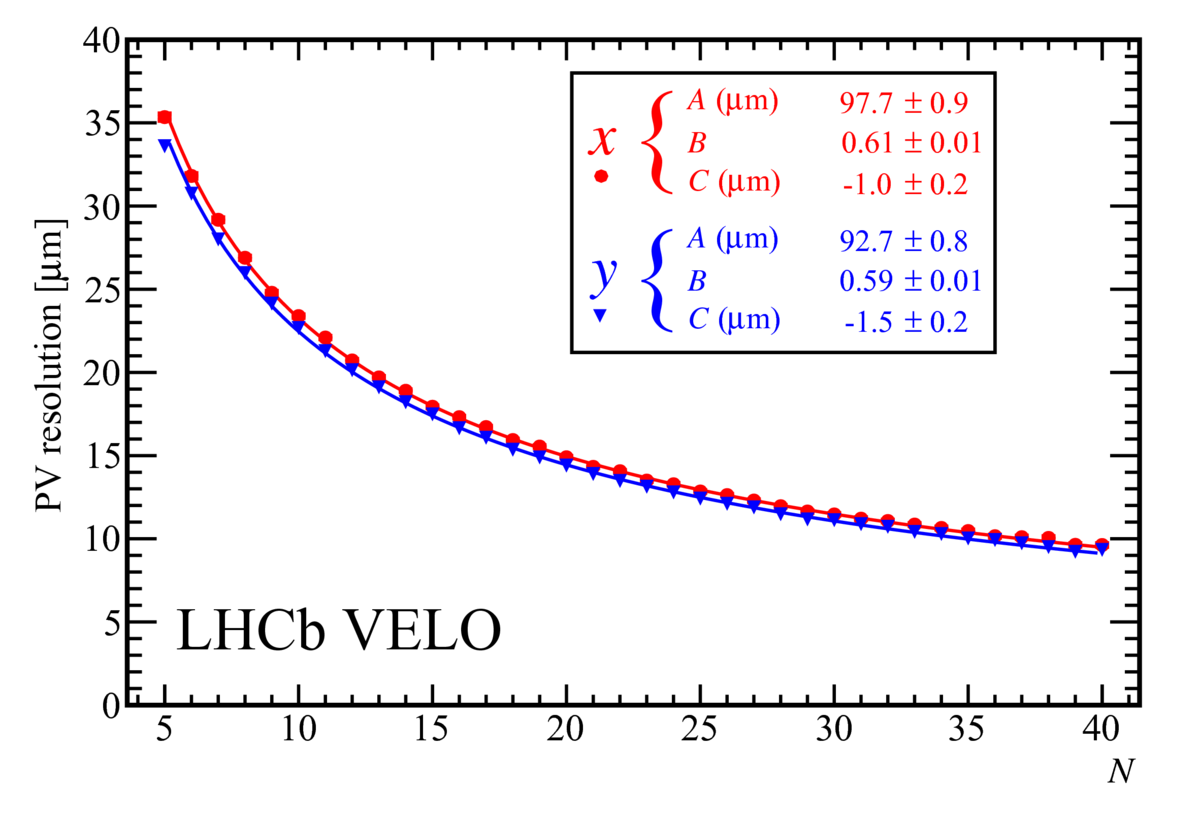
\includegraphics[ width=0.49 \textwidth]{./Figs/LHC_LHCb/hidef_ResXY_1PV_2011Data.png}
  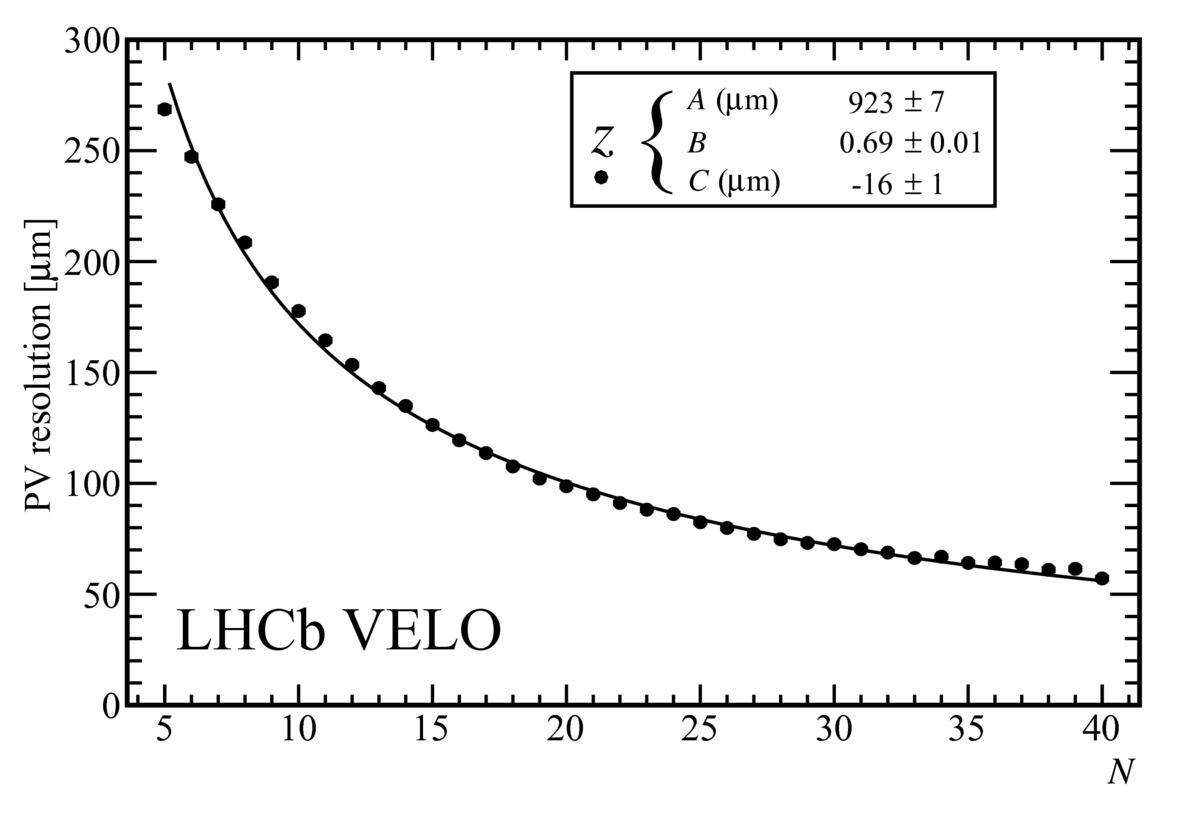
\includegraphics[ width=0.49 \textwidth]{./Figs/LHC_LHCb/hidef_ResZ_1PV_2011Data.png}

  \caption{Resolution of the position of vertices in an event achieved by the VELO in 2012 data. The resolution is shown for primary vertices perpendicular (left) and parallel (right) to the beam axis as a function of the number of tracks in an event~\cite{LHCbVELOGroup:2014uea}.}
  \label{fig:Velo_PV_resolution}
\end{figure}


\begin{figure}[tb] 
  \centering    
  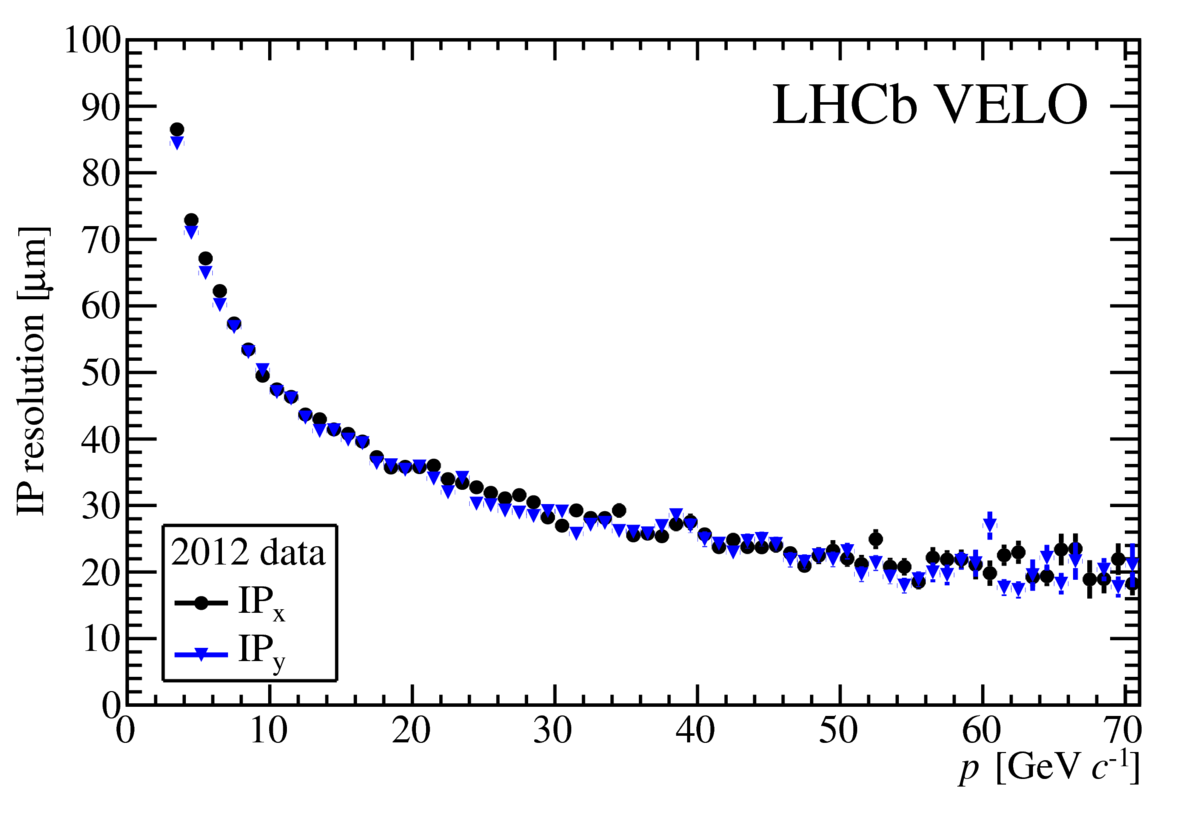
\includegraphics[ width=0.49 \textwidth]{./Figs/LHC_LHCb/hidef_IPRes-Vs-P-CompareIPxIPy-2012.png}
  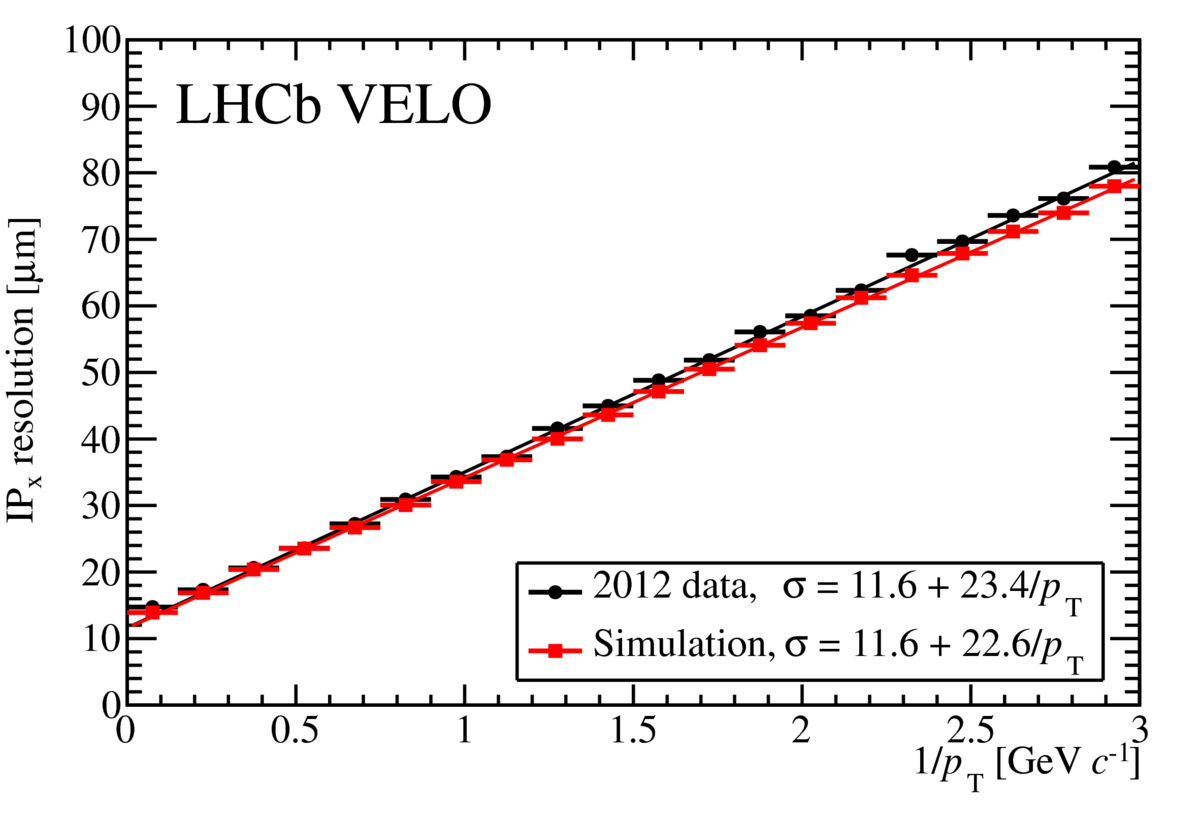
\includegraphics[ width=0.49 \textwidth]{./Figs/LHC_LHCb/hidef_IPXRes-Vs-InversePT-Compare2012DataToMC.png}
  \caption{Impact parameter resolution as a function of momentum (left) and inverse transverse momentum (right) achieved by the VELO for 2012 data~\cite{LHCbVELOGroup:2014uea}.}
  \label{fig:IP_res}
\end{figure}


%Overall the VELO gives such and such precision.  vertex resolution in the transverse plane 10-20 mircons, in the z directions 50-100 microns depending on the number of tracks in the vertex. %The VELO is also important the impact parameter resolution and decay time resolutions.  (This may go at the end so that everything for tracking is together?) best resolution is 4 micrometers which allows a lifetime measurement of 50 fs. (Performance paper)



\subsubsection{Tracking stations} 
\label{Tracking_Stations}
The LHCb experiment has 4 tracking stations in addition to the VELO. The Tracker Turicensis (TT) is located upstream of the magnet and the T stations, T1-T3, located downstream of the magnet~\cite{Barbosa-Marinho:582793, Barbosa-Marinho:519146}. These tracking stations provide complementary information to the VELO, and the presence of the magnetic field allows the momentum and the sign of electric charge of particles to be determined. 



The TT is made up of 4 layers of silicon trackers that cover the full LHCb angular acceptance. The TT is located just within the influence of the magnetic field of the dipole magnet, which provides the detector with two main purposes. First, the TT tracks the passage of charged particles with high momentum to enable good momentum resolution of tracks when the information is combined with that from other tracking stations. The TT has a resolution of 50~$\mu$m for a single hit. This resolution was chosen so that multiple scattering in the detector material rather than detector resolution is the limiting factor for the momentum resolution. The second purpose of the TT is to record tracks of low momentum particles that are then swept out of the detector acceptance as they continue through the magnetic field. These tracks will have a lower momentum resolution and help with pattern recognition within the RICH detectors. 
%Information from just the TT and the VELO can provide an momentum accuracy of ~ 20 $\%$. 
%active area of 8.4m^2


The T stations, T1-T3, use two different technologies. The central part of each station is covered by the Inner Tracker (IT), made of silicon, while the external part is covered by the Outer Tracker and composed of straw drift tubes. %are split into two sections. Each station is composed of an Inner Tracker (IT)~\cite{Barbosa-Marinho:582793} made of silicon and an Outer Tracker (OT)~\cite{Barbosa-Marinho:519146} composed of straw drift tubes. 
There is a large increase in the size of the tracking stations between the TT and the T3 to ensure all stations cover the full angular acceptance of the detector. The size of the TT is 150~cm~$\times$~130~cm and the T3 station is 600~cm~$\times$~490~cm. The relative sizes of the tracking stations are illustrated in Figure \ref{fig:size_of_tracking_stations} as well as the IT and OT sections of the T1-T3 stations. 
%Therefore the T stations are not composed of only silicon due to its high cost. % of silion. 
%The large size of the T stations meant that silicon was not used for the full coverage of each station due to its high cost.
\begin{figure}[tb] 
  \centering    
  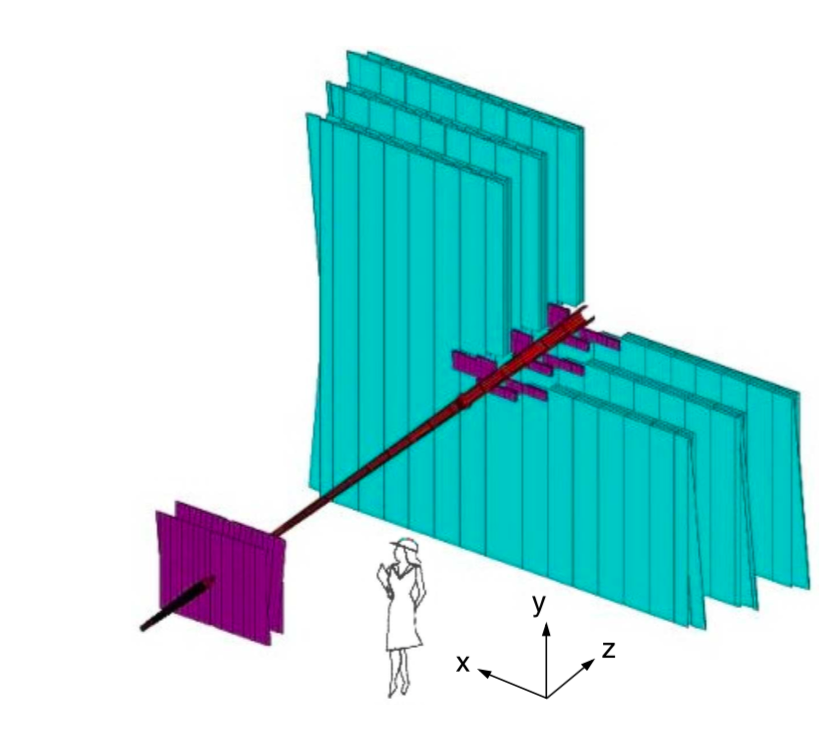
\includegraphics[ width=0.5\textwidth]{./Figs/LHC_LHCb/TT_IT_OT_comparison.png}
  \caption{Illustration of the relative sizes of the tracking stations. The TT is in magenta on the left hand side of the diagram, the IT is in purple surrounded in turquoise by the OT and the beam pipe is shown in red~\cite{Alves:2008zz}.}
  \label{fig:size_of_tracking_stations}
\end{figure}
The IT has very similar in design to the TT, each station is made of 4 layers of silicon trackers with an overall track resolution of 50 $\mu$m.
%and has an active area of 4.0m2. 
The silicon trackers are arranged in a cross shape around the beam pipe, as shown in Figure \ref{fig:size_of_tracking_stations}. Although the IT covers less than 2$\%$ of the T stations, 20$\%$ of tracks pass through it. This allows the occupancy of the OT to be less than 10$\%$ enabling a good overall track resolution from the OT despite it not being made of silicon. The OT of each tracking station is made of 2 staggered layers of straw tubes, covering the remaining area required for full coverage of the LHCb angular acceptance, including tracks bent by the magnetic field. The straw tubes have a fast drift time of 50~ns giving a better than 200~$\mu$m track resolution. 


\subsubsection{Dipole magnet}
\label{Magnet}
A warm dipole magnet~\cite{Amato:424338} is used to measure the momentum and electric charge of particles travelling through the LHCb detector. The magnet was designed to have an integrated field strength of 4~Tm for track that travels 10~m through the detector.%In a magnetic field the trajectories of charged particles are bent and the particle momentum can be measured from the curve of the track. %from the radius of curvature of the particle track the particle momentum can be determined.

The magnet is located between the TT and the T stations and magnetic field influences all charged particles in the LHCb angular coverage. The field is in the vertical direction therefore bending tracks in the horizontal direction. The magnet was designed so that the field strength in the RICH detectors is negligible (less than 2 mT) and to have the largest strength possible between the TT and T stations. Figure \ref{fig:Magnet_field} shows a plot of the magnet strength along the length of the detector. %A small magnetic field is achieved in the RICH detectors by iron shielding. The magnet was designed to have an integrated field strength is 4~Tm for track that travels 10~m through the detector.% and the peak strength is 1.1T. % I should maybe mention the measurement of the field and how it had to be accurate (with Hall probes) in order to get good momentum resolution but I don’t want to. The magnetic field strength enables the tracking systems to achieve a momentum resolution of $\delta p / p \~0.4\%$. 

\begin{figure}[tb]
  \centering
  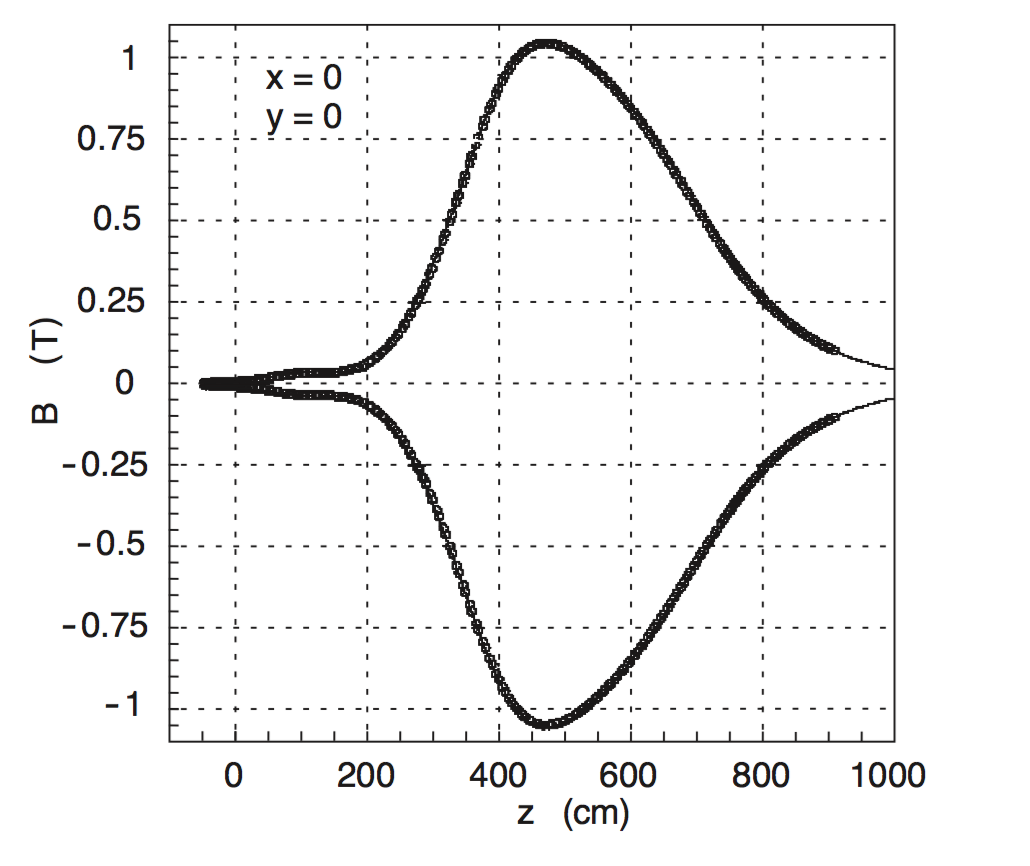
\includegraphics[ width=0.6\textwidth]{./Figs/LHC_LHCb/Magnet_field.png}
%  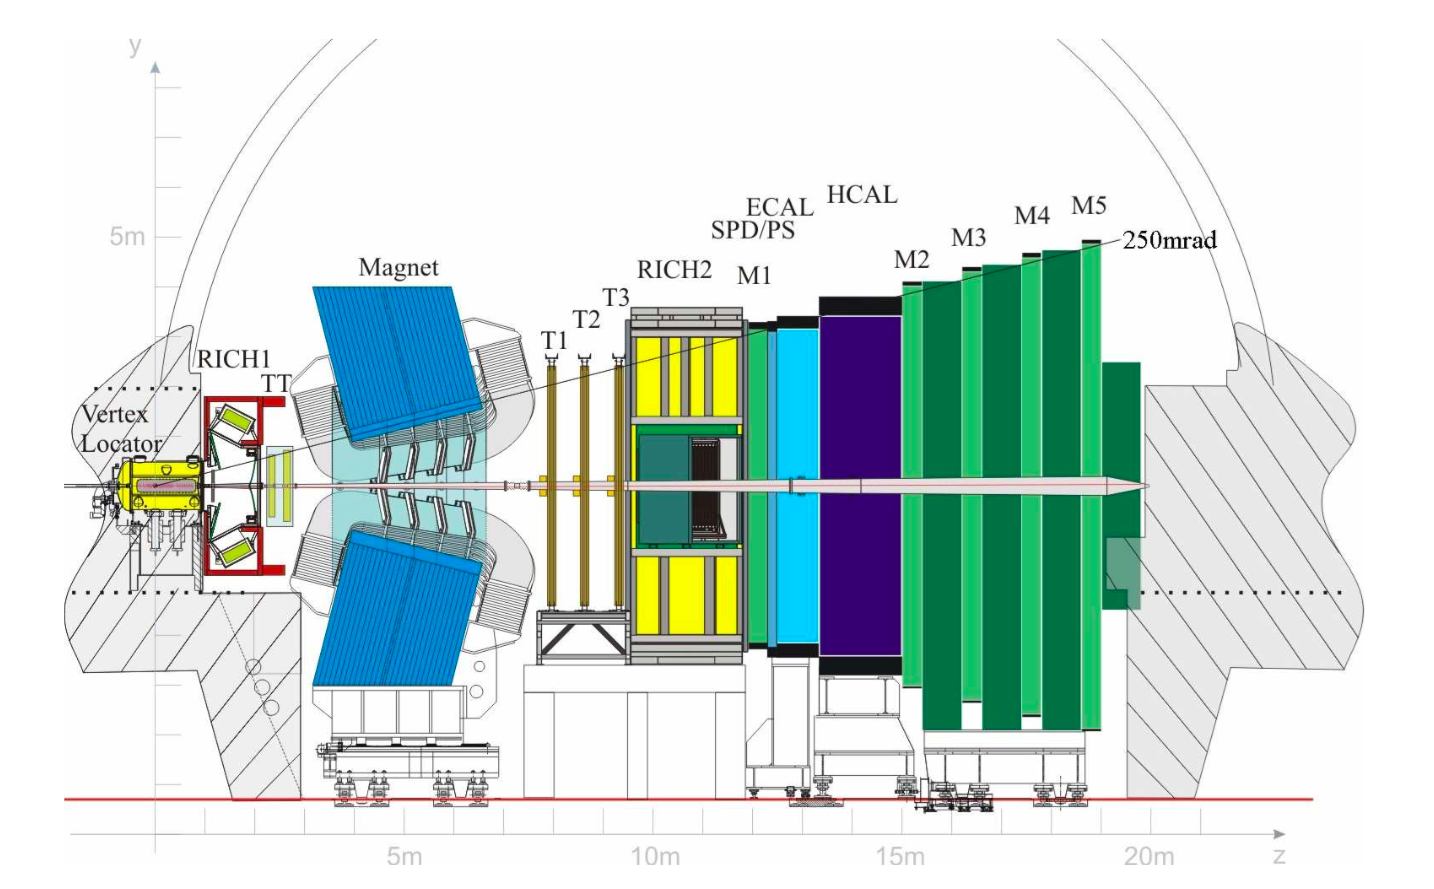
\includegraphics[ width=0.48\textwidth]{./Figs/LHC_LHCb/lhcb.png}
  \caption{Magnet field of the dipole magnet along the length of the LHCb detector. The peak strength of the field occurs between the TT and T1-T3 station. }
  \label{fig:Magnet_field}
\end{figure}

%\begin{figure}[tb] 
%  \centering    
%  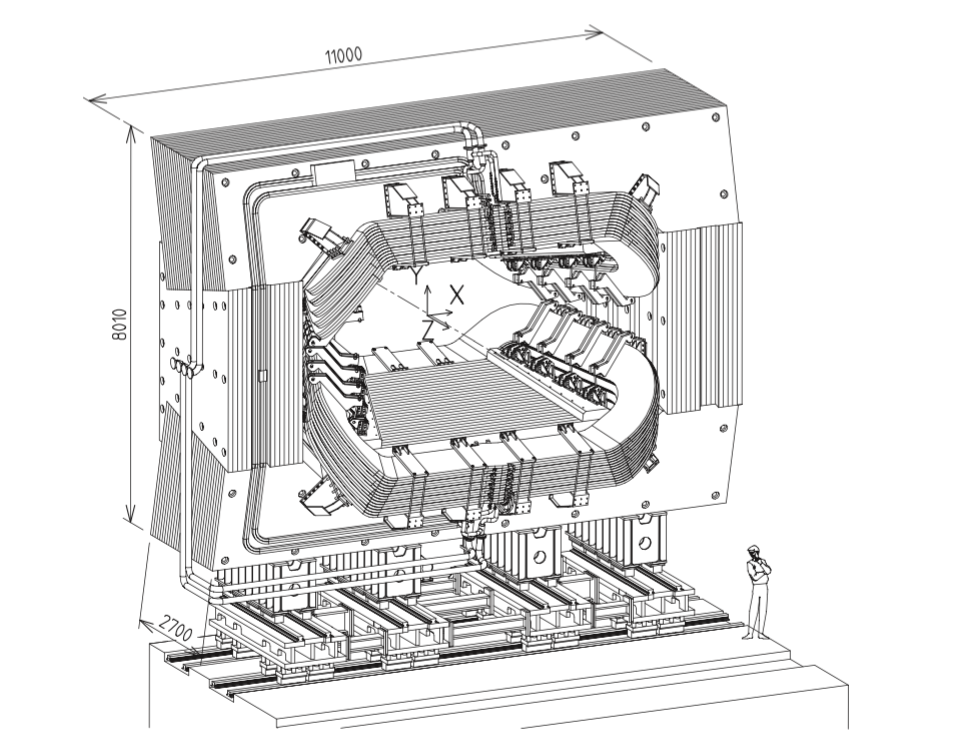
\includegraphics[ width=1.0\textwidth]{./Figs/LHC_LHCb/Magnet_picture.png}
%  \caption{Magnet picture. Source: \cite{Alves:2008zz}.}
%  \label{fig:types_of_tracks}
%\end{figure}


The polarity of the magnetic field is periodically switched so that charged tracks are bent in the opposite direction. The polarity is switched to enable approximately equal amounts of data to be recorded for each magnet polarity during every year of data taking.
%so that it bends charged tracks in opposite directions. 
This is done to measure detection asymmetries in each half of the detector and to help understand systematic uncertainties of $\mathcal{CP}$ violation measurements. % These are not relevant for B2mm.
%The magent polatrity is swtiched so that approximately equal amounts of data is recorded for each magnet polarity in a year. 


\subsubsection{Track reconstruction and performance}
\label{sec:Track_recon}


The information left by the passage of charged particles through the VELO, TT and T stations is combined using track reconstruction algorithms to find trajectories of charged particles through the length of the LHCb detector and infer the particle momentum.  
The tracking algorithms start with either segments of tracks in the VELO or the T stations and extrapolate from these segments into the other tracking detectors using specific search windows. 
Once all the segments of a track have been found, the trajectory is fitted with a Kalman Filter~\cite{Kalman,Fruhwirth:1987fm} which takes into account multiple scattering and energy loss within the detector. For each track the Filter returns the $\chi^{2}$ per degree of freedom, which is a measure of quality for the track. This parameter is used to ensure that only good quality tracks are used in physics analyses. 
The reconstructed tracks are classified into five types depending on which detectors they travelled through, as shown in Figure~\ref{fig:tracks}.

\begin{figure}[tb]
  \centering
  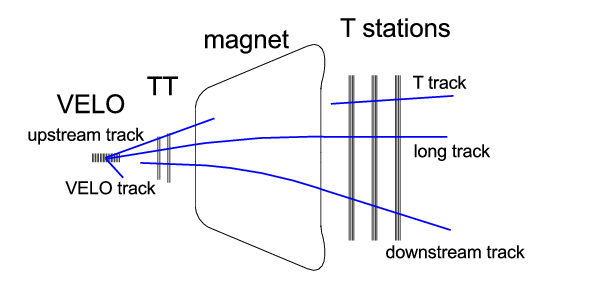
\includegraphics[ width=0.8\textwidth]{./Figs/LHC_LHCb/Types_of_tracks.png}
  \caption{Different types of tracks that are reconstructed at the LHCb experiment~\cite{Aaij:2014pwa}.}
  \label{fig:tracks}
\end{figure}

The different track classifications are:
\begin{itemize}
\item  VELO tracks are formed by particles produced at large angles to the beam axis or travelling in the negative $z$ direction from the interaction point, therefore these particles only leave tracks in the VELO. VELO tracks are useful for reconstructing primary vertices;  
\item Upstream tracks are made by low momentum particles that leave hits in the VELO and TT stations. The absence of hits further down the detector is because the magnetic field sweeps the particles out of the detector acceptance. Upstream tracks have poor momentum resolution but are useful for understanding backgrounds and pattern recognition in the RICH-1 detector located between the VELO and the TT;
\item Downstream tracks are produced by the decays of long-lived neutral particles, that travel out of the VELO before decaying. These particles only leave tracks in the TT and T stations; 
\item T tracks are tracks that cross only the T1-T3 stations and are formed from particles created in interactions with the detector material. Similar to upstream tracks, T tracks can help to understand backgrounds and pattern recognition in the RICH-2 detector located just before the T stations; and
\item Long tracks are the most useful for understanding particles decays recorded by the detector because they are formed by particles that travel through the VELO, TT and T1-T3 stations. Information from all the tracking stations is combined in these tracks therefore they have the best momentum resolution.
\end{itemize}


%\begin{figure}[tb] 
%  \centering    
%  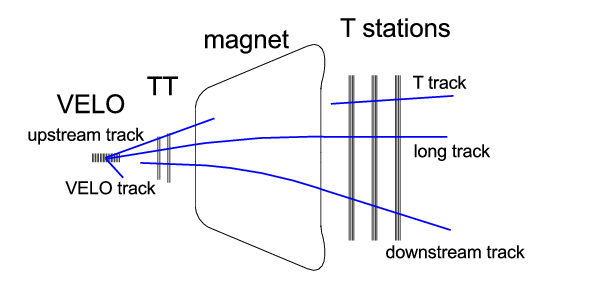
\includegraphics[ width=0.8\textwidth]{./Figs/LHC_LHCb/Types_of_tracks.png}
%  \caption{Different types of tracks that are reconstructed at LHCb~\cite{Aaij:2014pwa}.}
%  \label{fig:types_of_tracks}
%\end{figure}

The efficiency to correctly reconstruct tracks varies with the particle momentum and the number of tracks present in an event, as shown in Figure~\ref{fig:types_of_tracks} for 2012 data. In Run 1 long tracks were correctly reconstructed an average of 96$\%$ of the time.





\begin{figure}[tb] 
  \centering    
  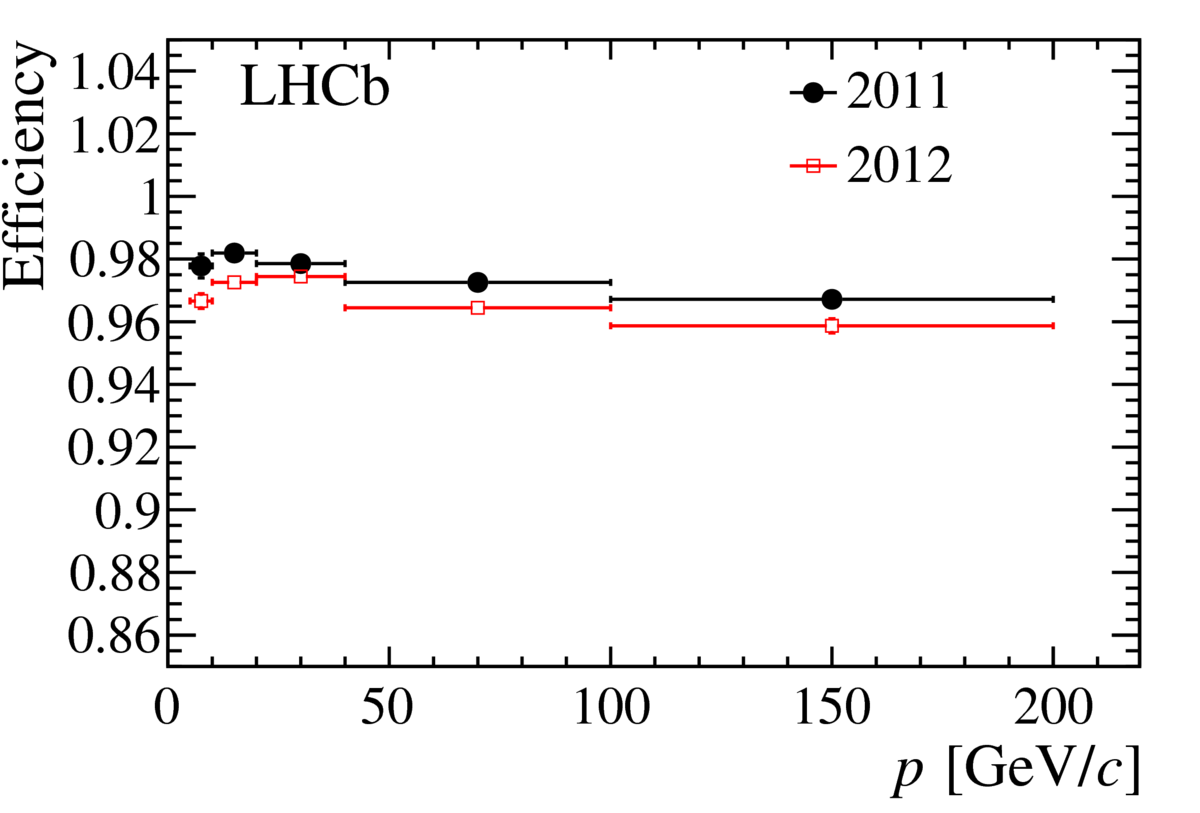
\includegraphics[width=0.49\textwidth]{./Figs/LHC_LHCb/hidef_Fig16topleft.png}
  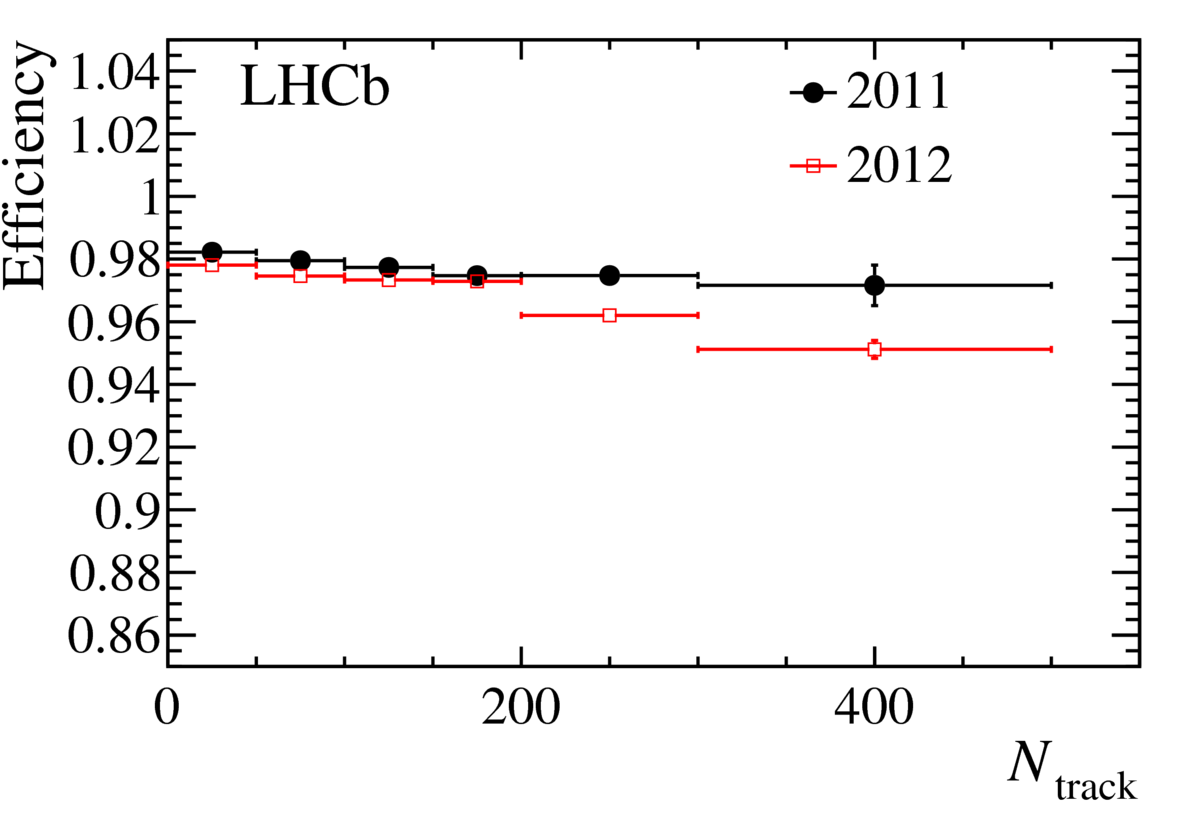
\includegraphics[width=0.49\textwidth]{./Figs/LHC_LHCb/hidef_Fig16bottomleft.png}
  \caption{Long track reconstruction efficiency as a function of momentum (left) and number of tracks in the event (right) for 2012 data \cite{Aaij:2014pwa}.}
  \label{fig:types_of_tracks}
\end{figure}




Inevitably not all tracks that are reconstructed are correct, there are two main types of incorrectly reconstructed tracks. The first are clone tracks that occur when two tracks have many hits in common. When this happens the track with the highest number of total hits is kept and the other is discarded. The second type are ghost tracks that are formed when track segments in different detectors are incorrectly joined together. This most often occurs with segments in the VELO and T1-T3 stations, the number of ghost tracks in an event depends on the event multiplicity. These tracks are removed by cutting on the output of a neural network that returns a probability of how likely a track is to be a ghost. %In Run 1 long tracks were correctly reconstructed an average of 96$\%$ of the time.



%Once the tracks have been reconstructed, parameters that are necessary for identifying and measuring different particle decays in an event can be computed from the tracks. 
The combined tracking systems achieve a momentum resolution of $\delta p / p = 0.5\%$ for particles with $p$ =  20~GeV/c and a resolution of $\delta p / p = 0.8\%$ for particles with $p$ =  100~GeV/c.  This momentum resolution, when combined with vertex information from the VELO, gives a decay time resolution of around 50~fs~\cite{Aaij:2014jba}. 



%The performance of the tracking system has been studied of Run 1 data \ref{ performance paperS}. The tracking system provide measurement of the momentum of the charged particles that it tracks, good momentum resolution is required in order to obtain good mass resolution which is necessary to identify different  b hadrons and to distinguish between signal and background events. The momentum resolution of long tracks is shown in figure  OR the momentum resolution is $\delta$p/p = X - Y $\%$ which depends on the momentum of the reconstructed track. 


%The tracking system allows accurate reconstruction of primary vertices, this is necessary to measure time dependant processes, lifetimes and identify decaying particles. It was particular important for LHCb so that is could measure the rapidly oscillation Bs system. The PV resolution has been measured on 2012 data and varies with the number of tracks used to reconstruct the vertex, on average the vertex resolution transverse to the beam is between 10 and 25 mum and parallel to the beam is  between 50 and 150 mum for the z direction as shown in figure \ref{fig:types_of_tracks} for 2011 data. %Ref veto paper.



%The impact parameter is another important variable, it measure the distance of closest approach of a track to the PV, long lived particles tend to have a large IP wrt to PV because they travel before they decay. Good measurements of the IP help to remove prompt backgrounds. The IP resolution depends on the momentum of the particles and Figure \ref{fig:types_of_tracks} shows the IP resolution for 2012 data, for a track with transverse momentum of 1 GeV/c is has an IP resolution of 35 mum.

%Finally, the measurement of lifetime of b hadrons at LHCb needs accurate decay time measurements but more importantly to understand the rapidly oscillating Bs system good decay time resolution is needed. To reconstruct the decay time information about particle momentum and decay length, how far the particle travelled before it decays are needed. Therefore good PV resolution and moment resolution are needed. The LHCb detector achieved typically 50 ns resolution on the decay time. 



\subsection{Particle identification}
\label{PID}
The particle identification (PID) detectors consist of two Ring Imaging CHerenkov (RICH) detectors, electromagnetic and hadronic calorimeters, and muon stations. Together these detectors distinguish between different charged leptons and hadrons and between neutral particles such as photons and neutral pions. Good particle identification is necessary to determine which \bhadron decayed and to distinguish between topologically similar decays, such as \bdkpi, \bskk and \bmumu decays. %This could be out elsewhere perhaps in the RICH specific part?
The separate particle identification detectors are described in Sections~\ref{RICH}, \ref{Calo} and~\ref{Muon_stations} and the methods used to combine information from each detector to identify different particle types is described in Section~\ref{PID_variables}. 


\subsubsection{Ring Imaging Cherenkov detectors}
\label{RICH}
%There is a plot that shows the usefulness in comparing 2 mass plots of the RICH PID, this is in Ed Greening's Thesis. It could be nice to include this, or something like it because it is very relevant to Bs2MuMu and the verification of the lifetime measurement methods that I did. 

The LHCb experiment uses two RICH detectors~\cite{Amato:494263,Adinolfi:2012qfa} that are shown in Figure~\ref{fig:RICH_diagram}.
The RICH-1 detector is located between the VELO and the TT station and RICH-2 detector is located between the last tracking station and the first muon station.
 Together the detectors provide particle identification information for particles that fall in the momentum range of 2 to 100~\gevc.
%RICH detectors~\cite{Amato:494263,Adinolfi:2012qfa} are used at LHCb to distinguish charged hadrons and leptons that have a momentum between 2 and 100~GeV/c. 
The RICH detectors are vital to distinguish between pions, kaons and protons frequently produced in \bhadron decays. %This needs to be done because correctly reconstructing the b hadron invariant mass relies on correctly identifying what it decayed into. Information from the RICH is particularly important at distinguishing different b2hh decays which is useful for this thesis. 
The energy range of the RICH detectors was chosen to cover the momentum range of decay products coming from multi-body and 2-body $b$-hadron decays. %dbecause the typical decay products of 2-body and multi-body \bhadron decays is around 50~GeV. 

\begin{figure}[tb]
  \centering
  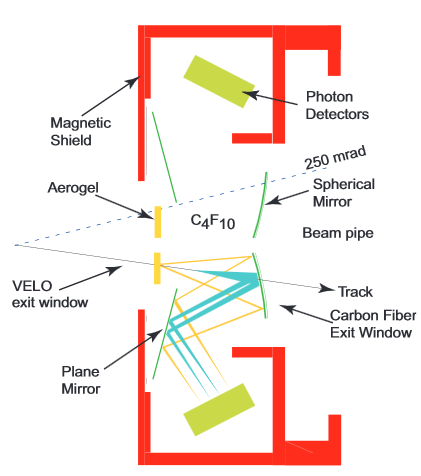
\includegraphics[ width=0.50\textwidth]{./Figs/LHC_LHCb/RICH1diagram.png}
  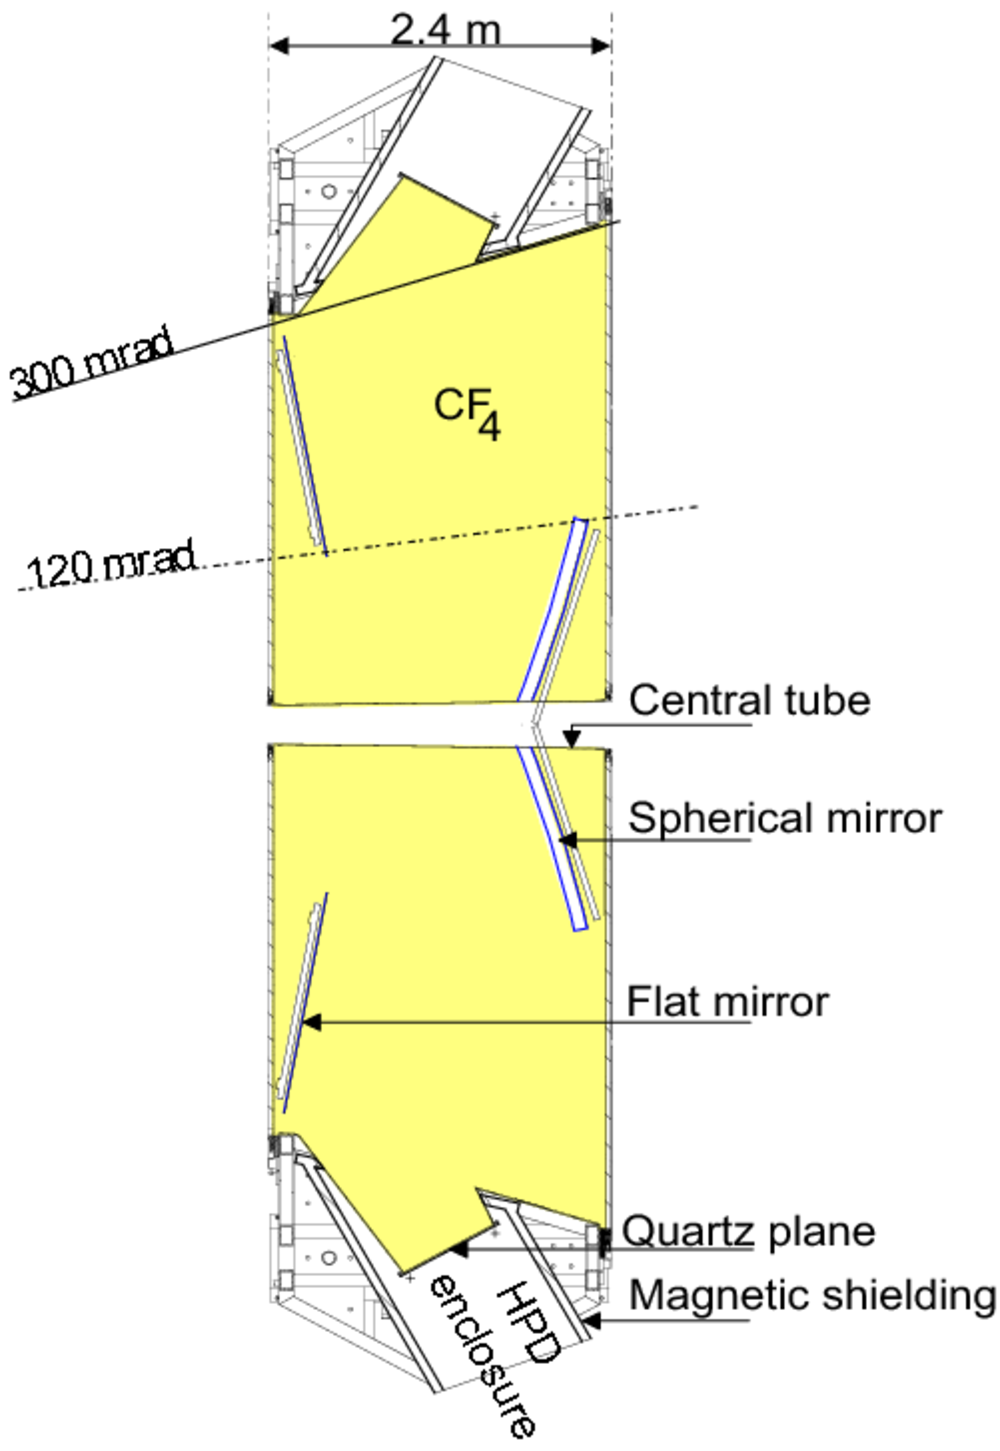
\includegraphics[ width=0.375\textwidth]{./Figs/LHC_LHCb/rich2_schematic.png}
  \caption{RICH-1 detector (left) and the RICH-2 detector (right)~\cite{Alves:2008zz}. For Run 2 the aerogel radiator in the RICH-1 detector was removed. }%Both RICH detectors use HPDs to detect light from Cheren that are sensitive to magnetic fields, the HPDs are shielded from the\magnet field using iron sheets ensuring the field is less than 2mT across them. This allows accurate detection of light created within the RICH detectors. 
  \label{fig:RICH_diagram}
\end{figure}

These detectors are based on the following principle; when a charged particle travels through a dielectric medium the atoms excited by its passage are polarised. If the particle is travelling faster than the speed of light in the medium, the excitation energy is released as a coherent wavefront. The angle the wavefront travels at relative to the particle trajectory, $\theta_{c}$, depends particle velocity, $v$ , and the refractive index of the medium, $n$, as $\cos(\theta_{c}) = c/nv$. The light is produced in a ring and is called Cherenkov radiation. %The RICH detectors measure the angle of light produced as particles pass through them, the angle gives a measurement of the particle’s speed which when combined with momentum from the tracking stations gives that particle’s mass and therefore its identity. 
The angle at which Cherenkov radiation is produced gives a measurement of a particle’s speed, which when combined with the particle’s momentum, as measured by the tracking detectors, the particle mass and consequently its identity can be determined. However, many particles travel through the RICH detectors and create overlapping rings of light making particle identification complex. As charged particles travel through RICH detectors, the rings of light produced are focused by spherical and planar mirrors onto Hybrid Photon Detectors (HPDs)~\cite{Alemi:1999np}, as shown in Figure~\ref{fig:RICH_diagram}. The radii of the detected rings provides information about how fast the particle was travelling.
Particle trajectories through the RICH detectors are inferred from information in the tracking stations and the expected pattern of Cherenkov radiation is calculated for each possible particle type. The expected patterns of light are compared to the observed pattern to find the likelihood for each particle type, all possible particle types are compared to maximise the likelihood. An in-depth description of the reconstruction algorithm used in the RICH detectors can be found in~\cite{Forty:684714}. 
%The performance of HPDs used in the RICH detectors is sensitive to the magnetic field of the dipole magnet.
%Both RICH detectors use HPDs that are sensitive to magnetic fields,                                                                          
%Therefore the HPDs are shielded from the using iron sheets ensuring the field is less than 2mT across them. %This allows accurate detection o\
%f The performance of HPDs used in the RICH detectors is sensitive to the magnetic field of the dipole magnet.
%Both RICH detectors use HPDs that are sensitive to magnetic fields, 
%Therefore the HPDs are shielded from the using iron sheets ensuring the field is less than 2mT across them. %This allows accurate detection of light created within the RICH detectors.

%\begin{figure}[tb]
%  \centering
%  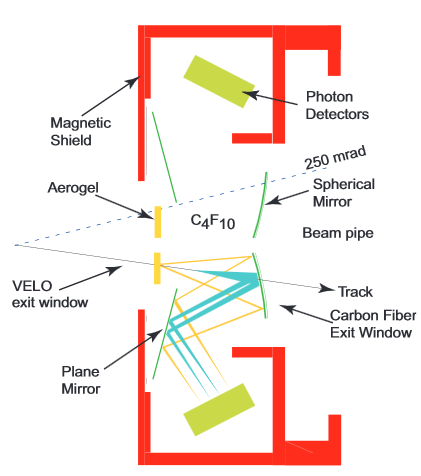
\includegraphics[ width=0.50\textwidth]{./Figs/LHC_LHCb/RICH1diagram.png}
%  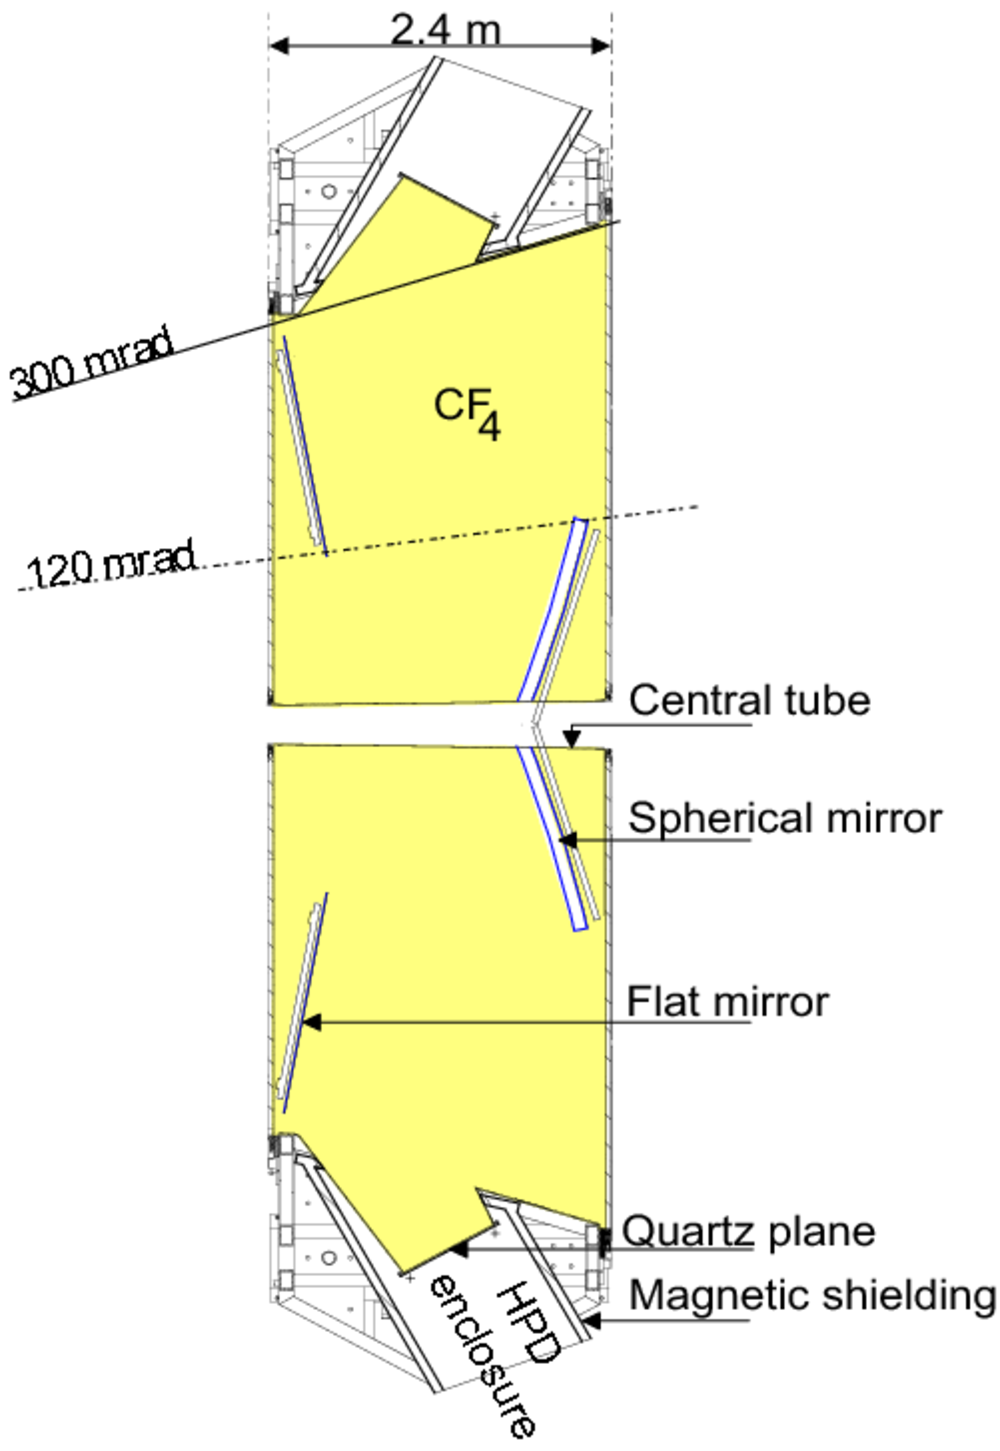
\includegraphics[ width=0.375\textwidth]{./Figs/LHC_LHCb/rich2_schematic.png}
%  \caption{RICH-1 detector (left) and the RICH-2 detector (right)~\cite{Alves:2008zz}. For Run 2 the aerogel radiator in the RICH-1 detector was removed. }%Both RICH detectors use HPDs to detect light from Cheren that are sensitive to magnetic fields, the HPDs are shielded from the magnet field using iron sheets ensuring the field is less than 2mT across them. This allows accurate detection of light created within the RICH detectors.
%%}%, also Olli has a nice picture of a HPD schematic.}
%  \label{fig:RICH_diagram}
%\end{figure}


The two RICH detectors provide identification information for different particle momentum ranges. The RICH-1 is sensitive to particles in the momentum range of 2 to 40~GeV/c and the RICH-2 is sensitive to particles in the range 15~-~100~GeV/c, to achieve this the detectors are made of different materials.  
The RICH-1 detector is composed of an array of 16 aerogel tiles sensitive to particles with a momentum between 2 and 10~GeV/c, behind the aerogel is a $\text{C}_{4}\text{F}_{10}$ gas radiator sensitive to particles in the momentum range 10 to 40~GeV/c. The aerogel radiator was removed after Run 1, therefore the RICH-1 is only sensitive to particles in the momentum range 10 to 40~GeV/c in Run~2. Unlike the RICH-1, the RICH-2 detector is composed of only one radiator, a $\text{C}\text{F}_{4}$ gas radiator.

As well as covering different momentum ranges the RICH detectors also have different angular acceptances. The RICH-1 covers the full LHCb angular acceptance whereas the RICH-2 covers $\pm$~120~mrad in the horizontal and $\pm$ 100 mrad in the vertical direction. 
Although the angular acceptance for the RICH-2 detector is smaller, the area it covers contains the higher momentum particles it is sensitive to because the low momentum particles have been bent out of the acceptance by the magnetic field.

The performance of HPDs used in the RICH detectors is sensitive to the magnetic field of the dipole magnet.
%Both RICH detectors use HPDs that are sensitive to magnetic fields,                                                                         
Therefore the HPDs are shielded from the using iron sheets ensuring the field is less than 2mT across them. %This allows accurate detection o 
%The RICH-1 detector is located between the VELO and the TT station, it covers the full LHCb angular acceptance and provides PID information on particles in the momentum range 2 to 40~GeV/c. The RICH-1 detector illustrated in Figure~\ref{fig:RICH_diagram}, contains two different radiator materials; at the front of the detector is an array of 16 aerogel tiles sensitive to particles with a momentum between 2 and 10~GeV/c, behind the aerogel is a $\text{C}_{4}\text{F}_{10}$ gas radiator sensitive to particles in the momentum range 10 to 40~GeV/c. The aerogel radiator was removed after Run 1, therefore the RICH-1 is only sensitive to particles in the momentum range 10 to 40~GeV/c in Run~2. As charged particles travel through RICH-1, the rings of light produced are focused by spherical and planar mirrors onto Hybrid Photon Detectors (HPDs)~\cite{}. The radii of the detected rings provides information about how fast the particle was travelling. %The speed of the particles, when combined with information about it’s momentum from the tracking stations realise the particles mass and therefore it’s identity.



%The RICH-2 detector is located upstream of RICH-1, between the last tracking station and the first muon station. RICH-2 consists of a $\text{C}\text{F}_{4}$ gas radiator sensitive to particles with a momentum range 15~-~100~GeV/c and the detection of the light produced is the similar to RICH-1, as illustrated in Figure~\ref{fig:RICH_diagram}. Unlike RICH-1, the RICH-2 detector does not cover the full LHCb angular acceptance but only $\pm$~120~mrad in the horizontal and $\pm$ 100 mrad in the vertical direction. This area contains the higher momentum particles the RICH-2 is sensitive to, the low momentum particles have been bent out of the acceptance by the magnetic field. 


%Both RICH detectors use HPDs that are sensitive to magnetic fields, the HPDs are shielded from the magnet field using iron sheets ensuring the field is less than 2mT across them. This allows accurate detection of light created within the RICH detectors.
 
The expected Cherenkov angles for particle types with different momenta  is shown in Figure~\ref{fig:RICH_radiator_predictions} for the radiator materials in the RICH detectors. % are shown in Figure~\ref{fig:RICH_preformance}.
The reconstructed Cherenkov angle as a function of momentum is shown in Figure~\ref{fig:RICH_preformance} for particles transversing the RICH-1 detector in 2011 data, the data shows distinct bands for each particle type as expected for the detector.

 
%The perforamance of the RICH-1 gas radidator on 2011 data 
%The rings of light collected by the RICH detectors when combined with information about particle momentum and tracks from the tracking stations enables the particle type to be identified. Figure \ref{fig:RICH_preformance} shows how the Cherenkov angle and momentum can be combined to identify different types of particles in the RICH-1 detector, there are distinct bands for each particle mass. Figure \ref{fig:RICH_radiator_predictions} shows what is expected for the different radiators.  
\begin{figure}[tbp]
  \centering
  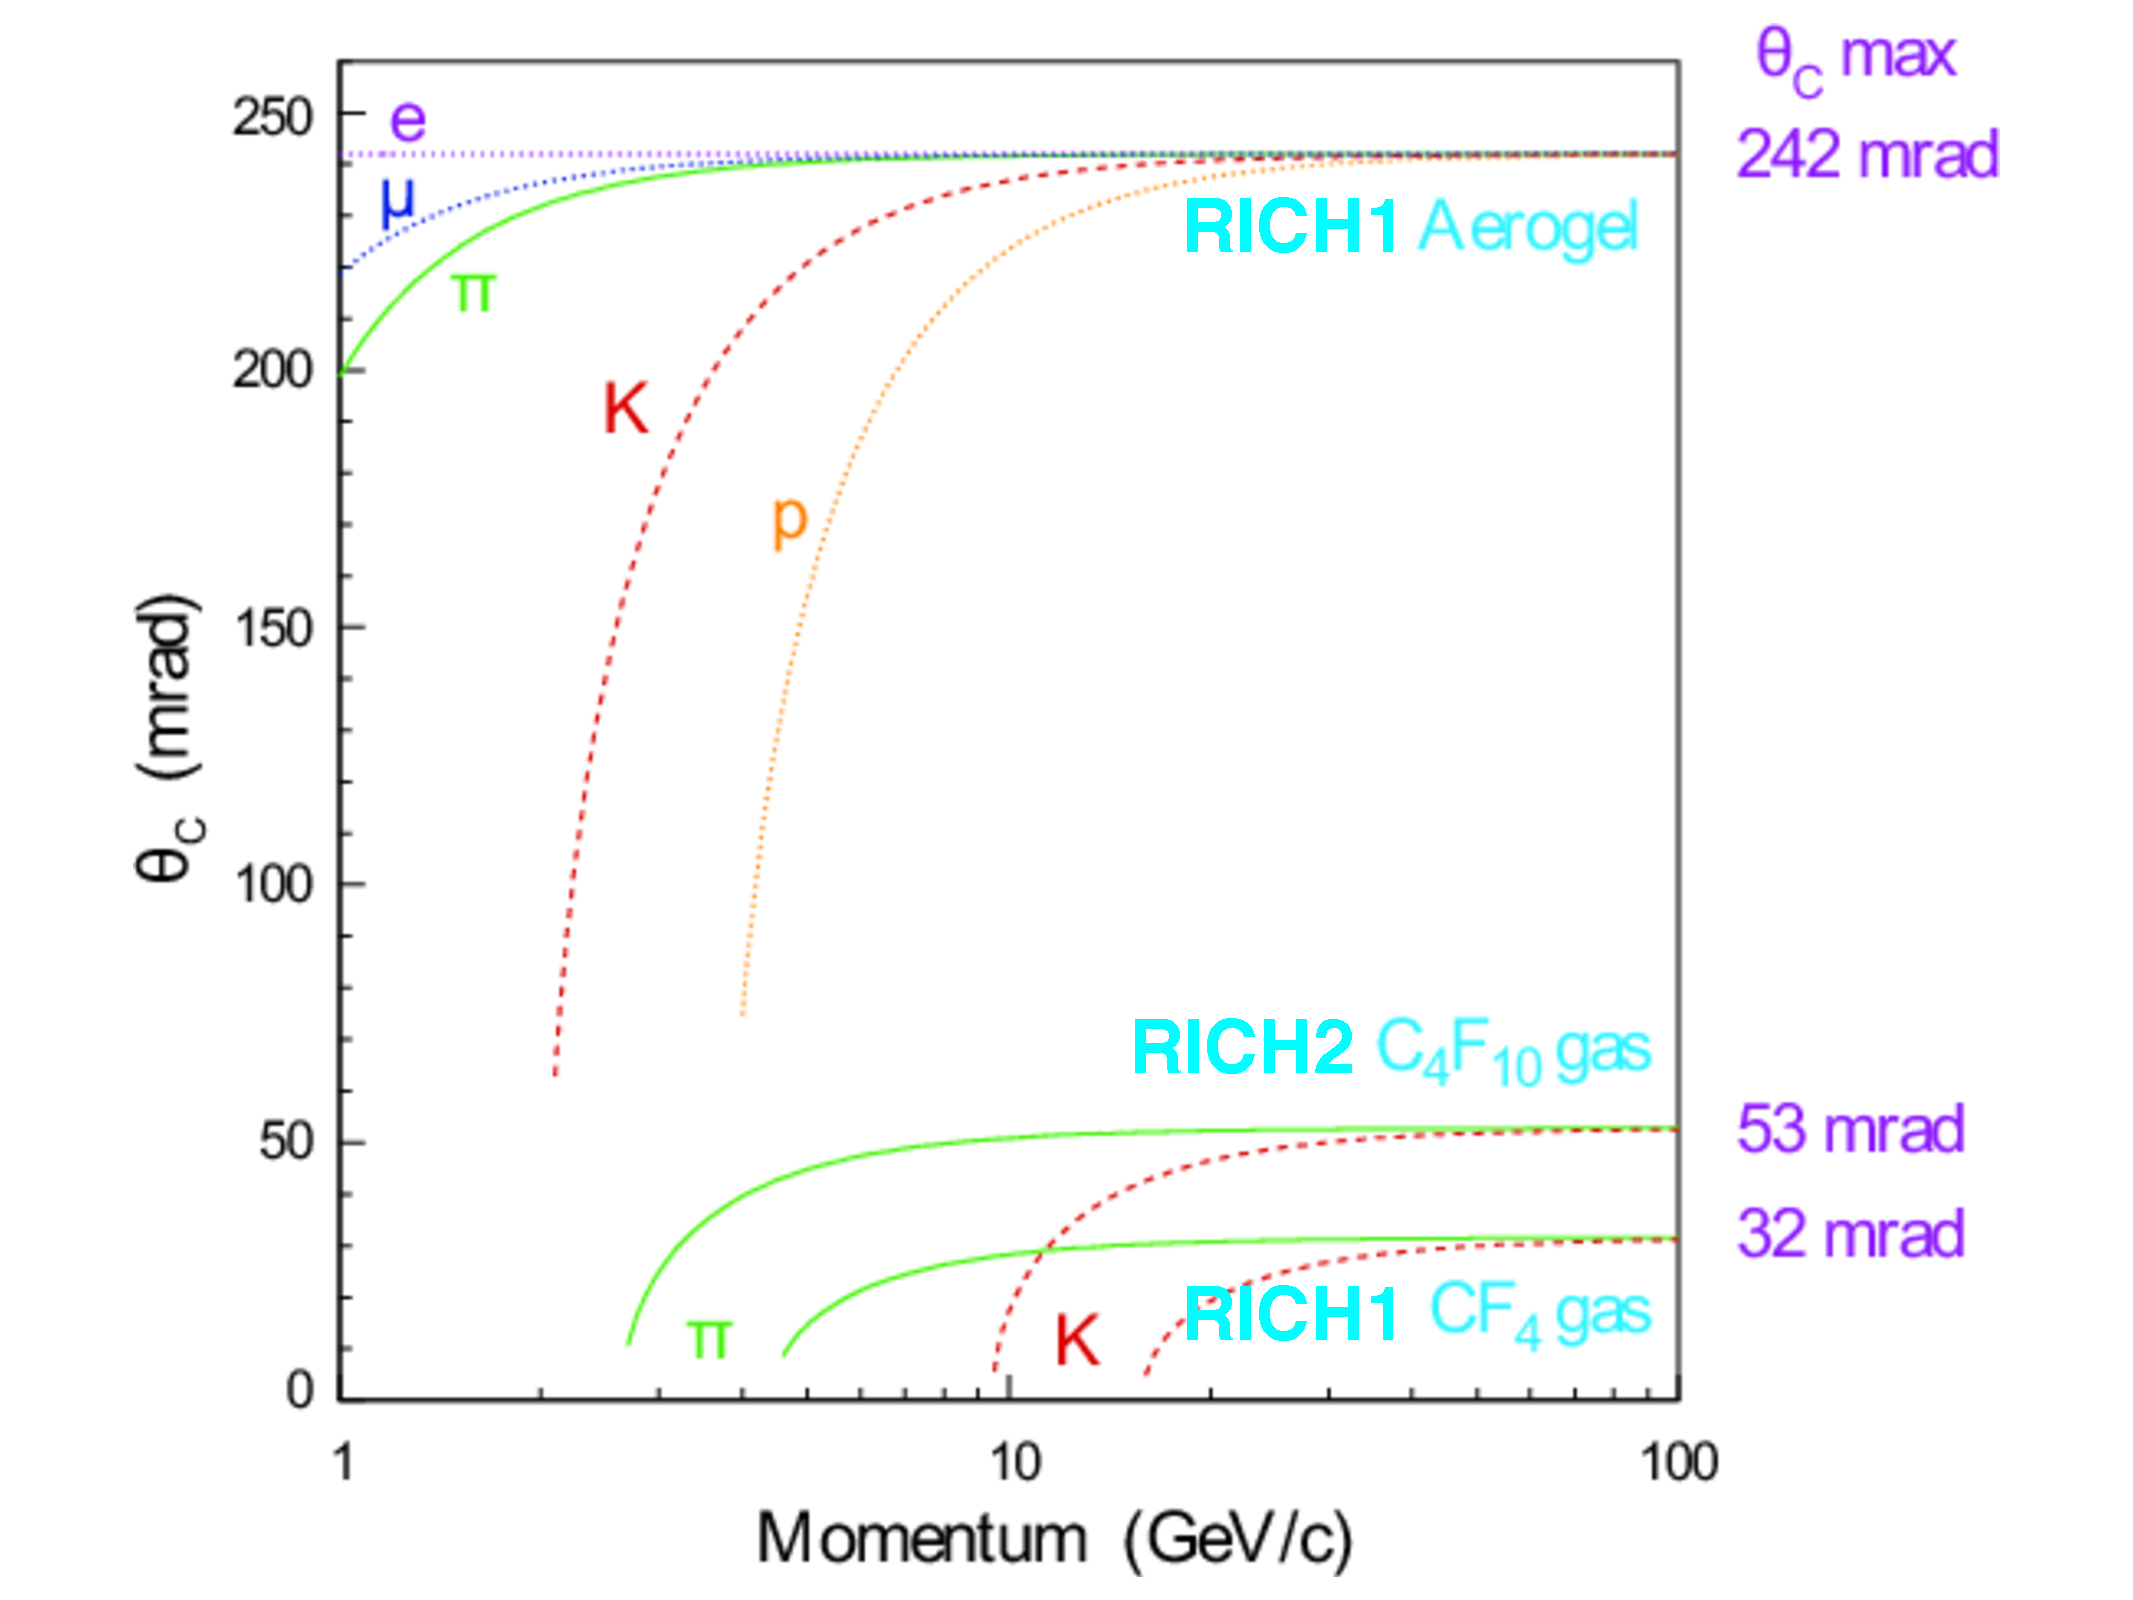
\includegraphics[ width=0.7\textwidth]{./Figs/LHC_LHCb/RICH_radiators.pdf}
  \caption{Expected Cherenkov angles produced by different particles travelling through the radiators in the RICH detectors~\cite{Alves:2008zz}.}
  \label{fig:RICH_radiator_predictions}
\end{figure}



\begin{figure}[tbp]
  \centering
  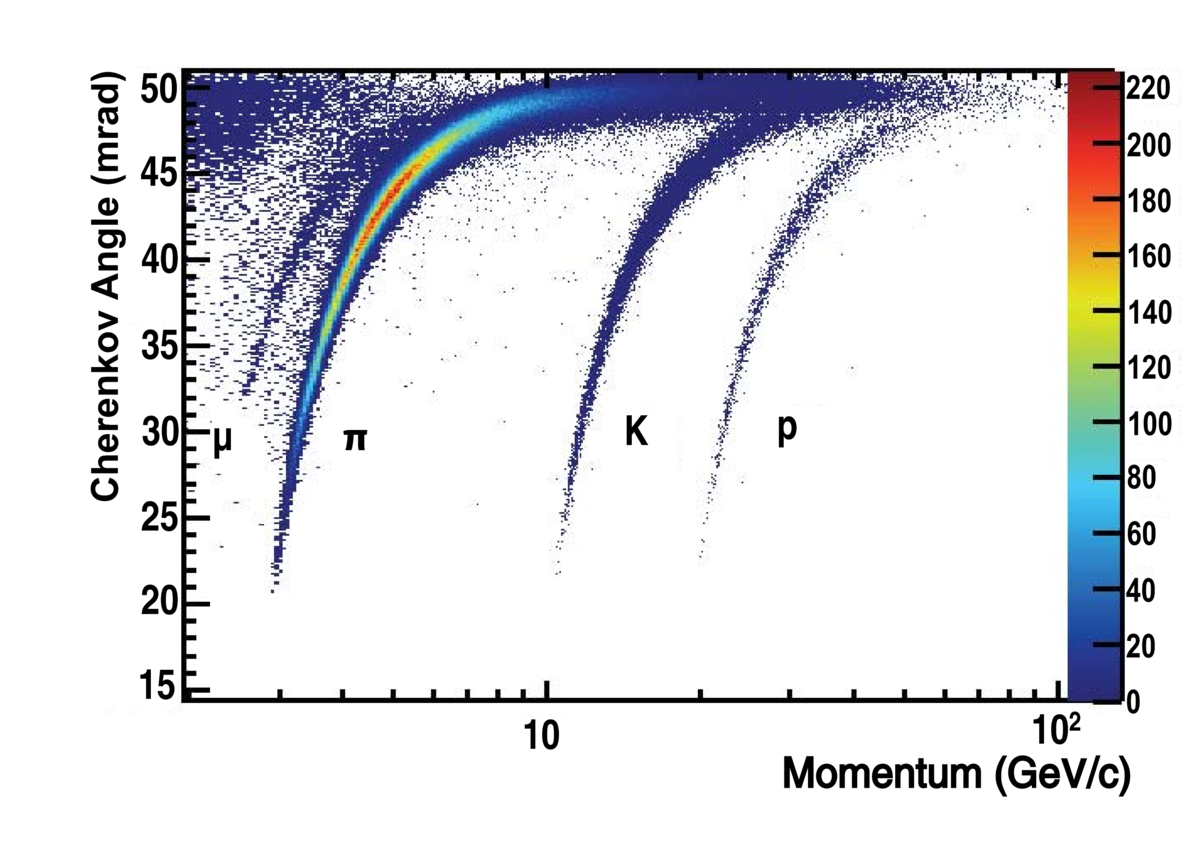
\includegraphics[width=0.8\textwidth]{./Figs/LHC_LHCb/hidef_Fig38.png}
  \caption{Cherenkov angles for isolated tracks as a function of momentum in the RICH-1 detector for 2011 data \cite{Adinolfi:2012qfa}.}
  \label{fig:RICH_preformance}
\end{figure}

%\begin{figure}[tbp]
%  \centering
%  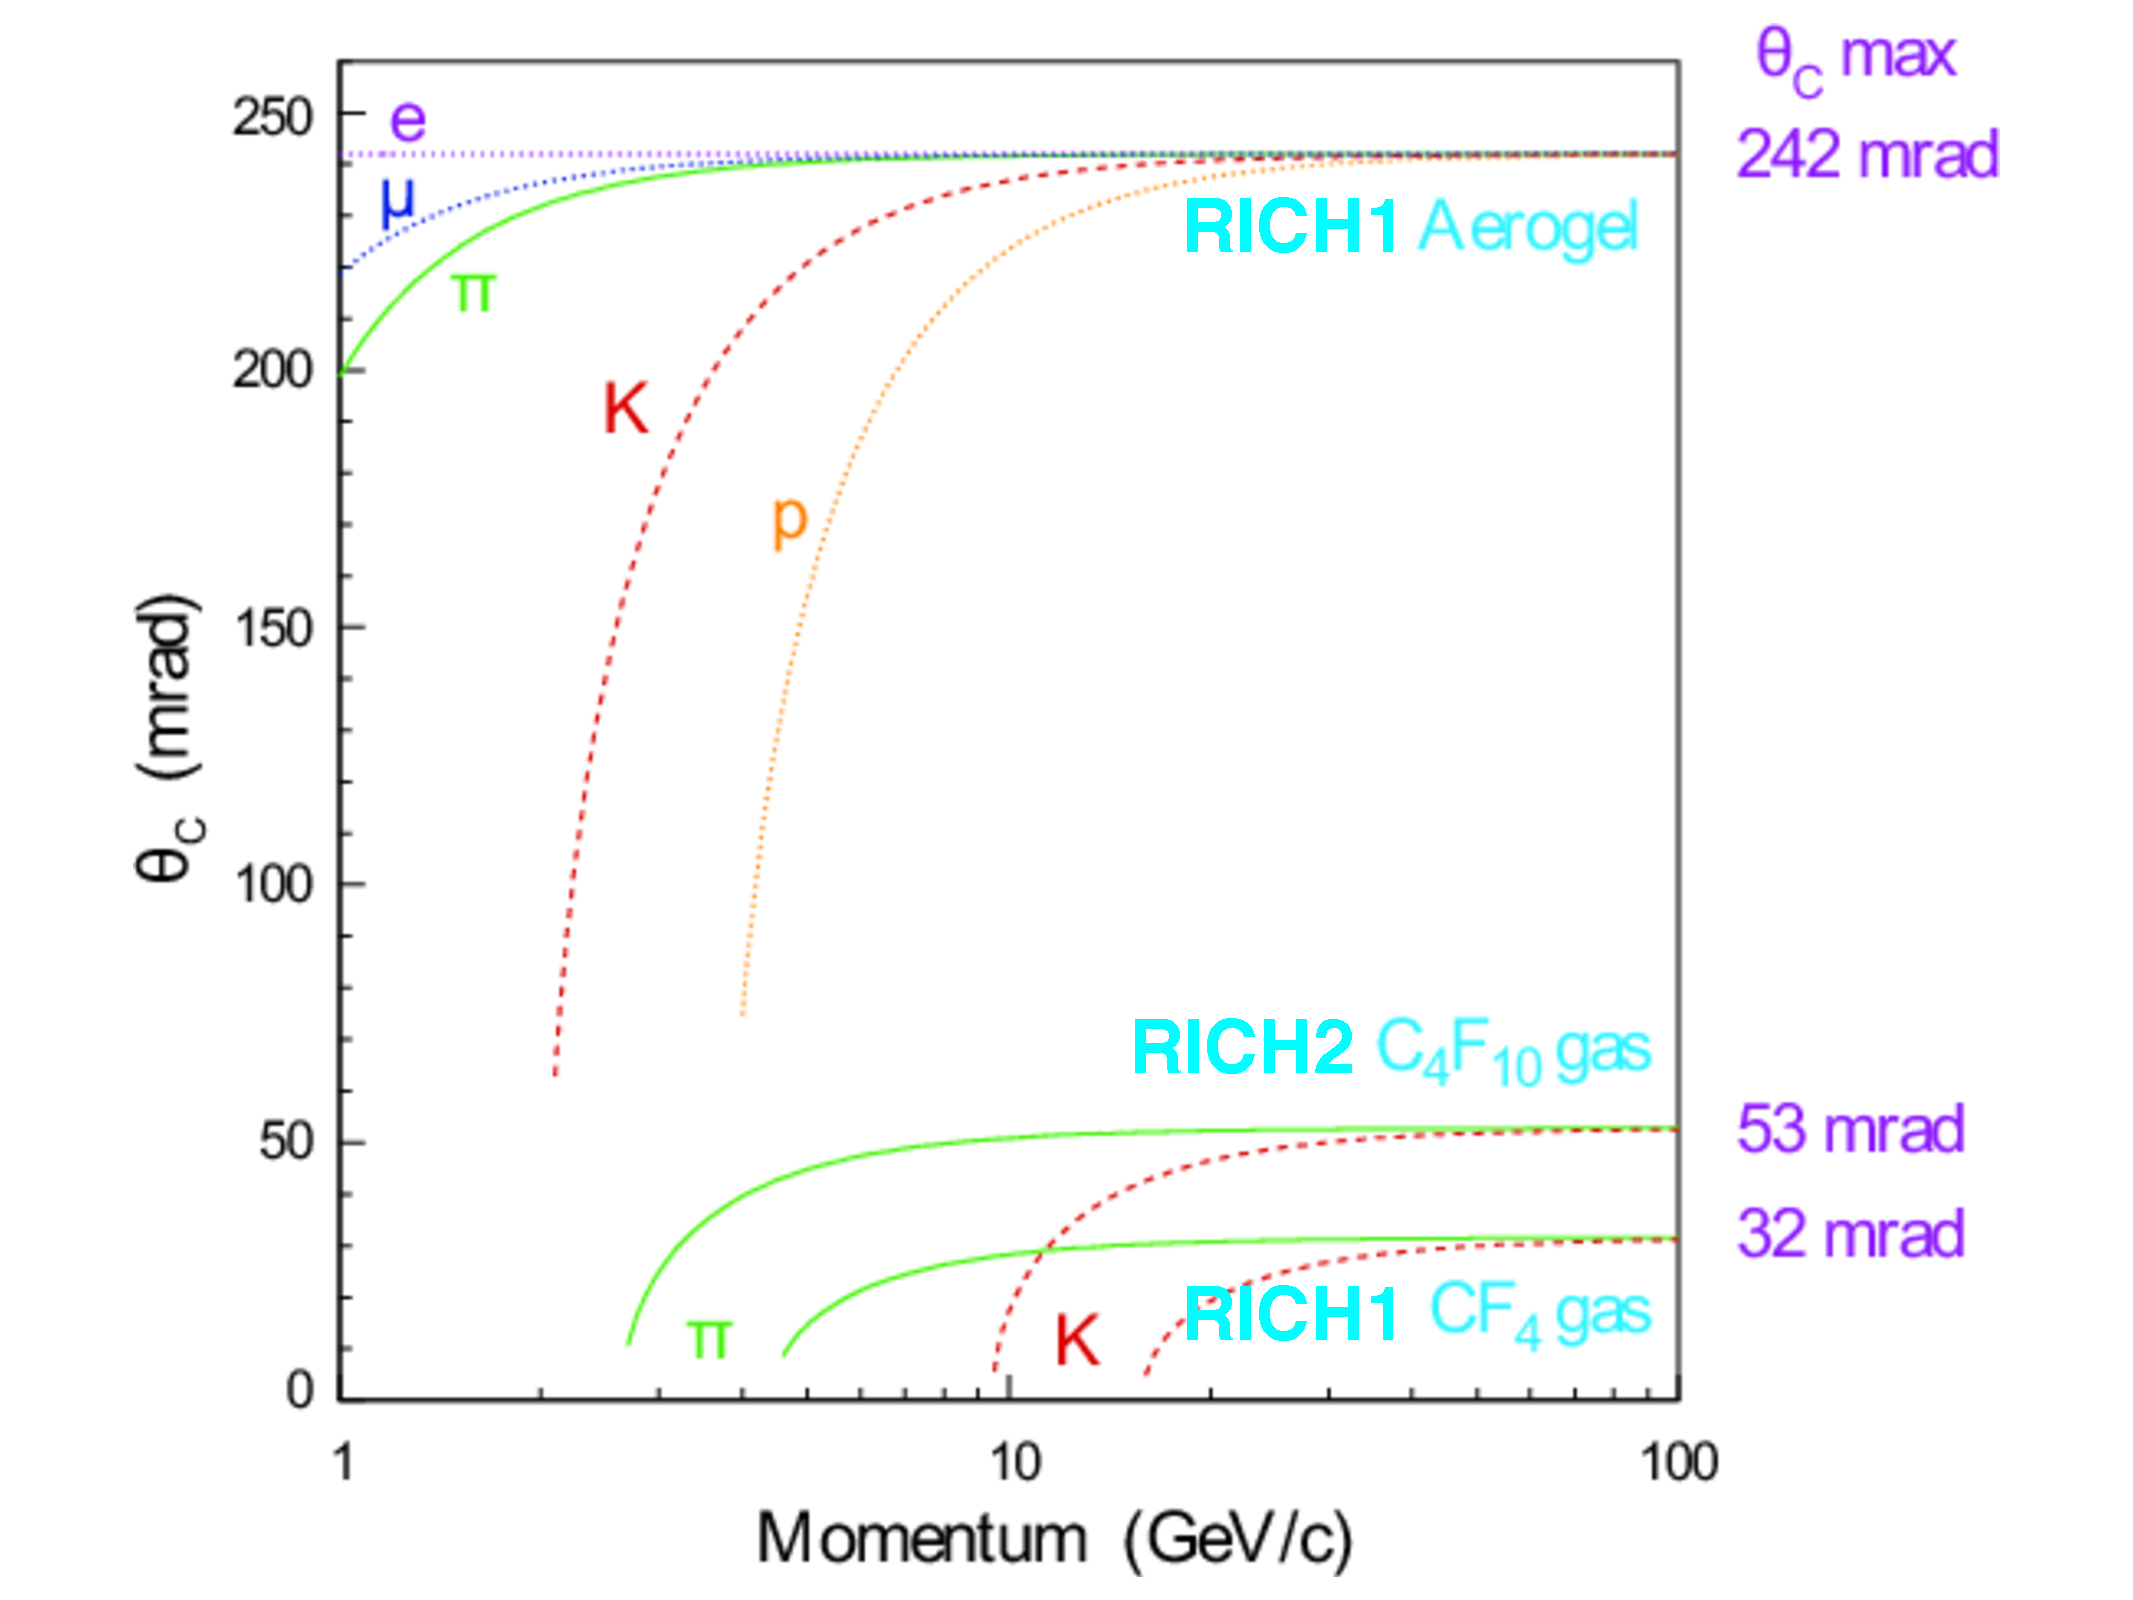
\includegraphics[ width=0.7\textwidth]{./Figs/LHC_LHCb/RICH_radiators.pdf}
%  \caption{Expected Cherenkov angles produced by different particles travelling through the radiators in the RICH detectors~\cite{Alves:2008zz}.}
%  \label{fig:RICH_radiator_predictions}
%end{figure}


\subsubsection{Calorimeters}
\label{Calo}

The calorimeter system~\cite{LHCB:2000ab} consists of four detectors: a Scintillating Pad Detector (SPD); a Pre-Shower (PS); an electromagnetic calorimeter (ECAL); and a hadronic calorimeter (HCAL). Information from the calorimeters is used to identify electrons, photons and hadrons with high transverse momentum to be used in the first level of the trigger and to help with the reconstruction and identification of these particles. The ECAL is particularly important in the reconstruction of photons and neutral pions because it is the only part of the detector that measures the energy and momentum of these particles. 

The calorimeters in LHCb are sampling calorimeters consisting of layers of lead absorbers and scintillating material. In lead, incident particles create showers of secondary particles, the charged particles produced in the absorbers create light as they pass through the scintillators. The light travels through wavelength shifters where it is collected by photo-multiplier tubes and turned into an electrical signal. Electromagnetic showers caused by photons, electrons or positrons are started by ionisation, bremsstrahlung radiation or pair production depending on the energy and the type of the incident particle. Hadronic showers are caused by the interaction of hadrons with the detector via the strong force which produces showers of secondary particles. The showers produced in the calorimeters are along the direction of flight of the incident particle. %zUnlike other sub-detectors in LHCb, the calorimeters change the particle as it moves through the detector in order to measure the energy.

The SPD, PS and ECAL identify electrons, positrons and photons. The SPD is a layer of scintillating material at the start of the calorimeter system. It separates electron and photon showers created later in the calorimeter because only charged particles will produce light in the SPD. Next in the calorimeter system is the PS, and consists of a lead absorber followed by another scintillator similar to the SPD. The length of the lead absorber is chosen so that electrons will start showers in the absorber but charged pions will not. There is only a 1$\%$ chance of a pion creating a shower in the PS. Information collected by the PS enables showers created by pions in the ECAL to be separated from those created by electrons and positrons. The ECAL is designed to contain the entire shower of high energy photons so that it can provide a good energy resolution for photons passing through the detector. The ECAL has an energy resolution of $\delta E / E = 9\%/\sqrt{E} \oplus 0.8\%$  provided information from the PS and SPD are used. 

The HCAL is predominately designed for use in the trigger and there is no requirement that the HCAL contains the full hadronic showers, therefore it was designed with a lower energy resolution of $\delta E / E = 69\% / \sqrt{E} \oplus 9\%$. 


\subsubsection{Muon stations}
\label{Muon_stations}

%The muon stations are designed to identify highly penetrating muons for use in the trigger and offline analyses. 
Muons are produced in many \bhadron decays; good muon identification is necessary to trigger events containing muons and to distinguish topologically similar decays such as \bmumu and \bdkpi in the analysis of particle decays. 
Compared with other particles, muons have a high penetrating power due to their relatively large mass and because they do not interact via the strong force, these properties are exploited in the muon detectors. There are five muon stations~\cite{Barbosa-Marinho:504326} located at the far end of the detector from the interaction point. %The information from these stations is used to identify muons that are used both in the trigger and in the analysis of particle decays in the data collected. %and is used in the to make decisions in the trigger.


The layout of the muons stations is shown in Figure \ref{fig:muon_system}. 
%There are 5 muon stations, M1-5, shown in Figure \ref{fig:muon_system} that track and identify muons. 
The first muon station, M1,  is located before the calorimeters. The inner section, where the fluence is greatest, is made of Gas-Electron-Multiplier detectors~\cite{Bencivenni:691604} and the outer section is made from Multi-Wire Proportional Chambers (MWPCs)~\cite{Botchine:2002ela}. The remaining stations, M2-5, are located after the HCAL, by which point most other particles have been absorbed by the calorimeters. These stations are made from MWPCs interleaved with 80~cm of lead absorber to filter out any remaining hadrons. %and between each station is 80cm of lead absorber ensuring only high energy muons pass through the muon detector. 



A muon must have a momentum of at least 3 GeV/c to pass through the calorimeters and the M2 and M3 stations. To travel through all the muons stations a muon must have a momentum of 6~GeV/c. 
%Momentum information from the muons stations is used to make decsions in the trigger because it is fast to reconstruct the hits in these stations. 
Momentum information collected in the muon stations can be used in the trigger because the stations lie outside the magnetic field, which allows for fast reconstruction of the tracks and a muons. M1 is located before the calorimeters to improve the transverse momentum measurement of the muons that is needed in the trigger.

%The first 3 stations have a high spatial resolution and provide track and transverse momentum information to be used in the trigger. M1 is located before the calorimeters to improve the transverse momentum measurement of the muons. The last two stations have a lower spatial resolution and are designed to identify muons with the greatest transverse momentum. 


After the muon stations there is an iron wall to stop any particles from travelling downstream of the detector. The active area of the muon stations increases with distance from the interaction point to ensure the full angular acceptance of the detector is covered. %Tracking information collected in the muon stations can be used in the trigger because the stations lie outside the magnetic field which allows for fast reconstruction of the tracks and a muons. 

\begin{figure}[tb]
  \centering
  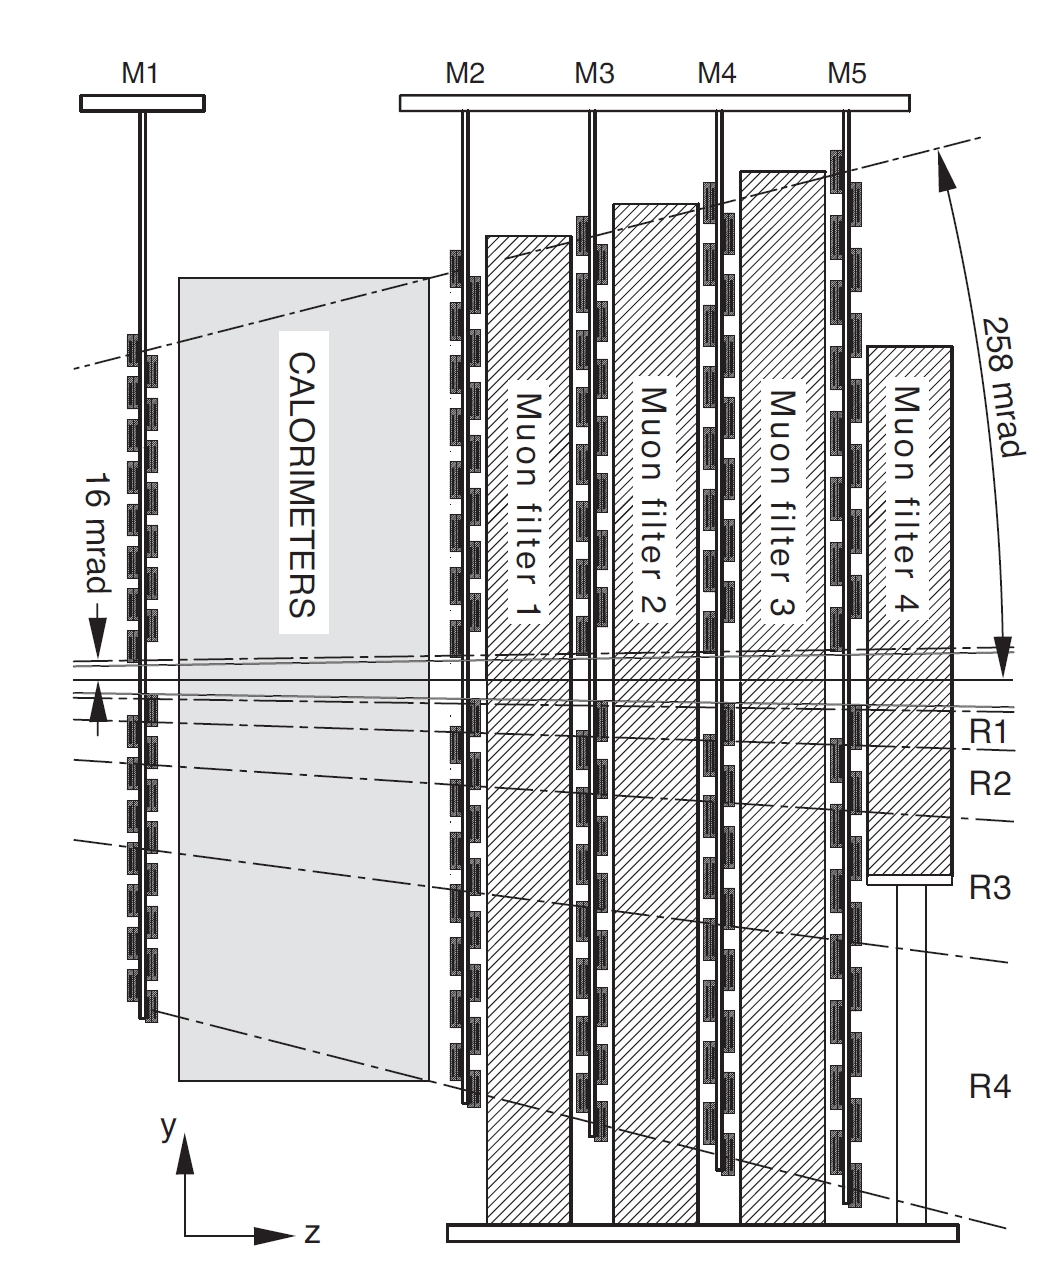
\includegraphics[ width=0.5\textwidth]{./Figs/LHC_LHCb/muon_system.png}
  \caption{Layout of the muon stations~\cite{Alves:2008zz}.}
  \label{fig:muon_system}
\end{figure}

\subsubsection{Particle identification and performance}
\label{PID_variables}
%There is a plot that shows the usefulness of the RICH PID, this is in Ed Greening's Thesis. 
%The information from the PID detectors is used to identify electrons, muons, protons, kaons and pions.  



The information collected in the PID detectors is combined to provide several discriminating variables that can be used to identify muons, protons, kaons, pions and electrons.
There are three types of variables: the isMuon criteria, DLL variables; and ProbNN variables, which are described in the following.
The performance of these variables at distinguishing between different particles types is described in detail in references~\cite{Aaij:2014jba,Archilli:2013npa}

The muon stations are used, along with information from the tracking system, to produce a binary selection to identify muons called the isMuon criteria. The tracking system is used to extrapolate a field of interest within the muon stations, a muon is identified if hits in the muon stations can be combined with those from the tracking system within the field of interest. The number of hits required in the muon stations depends on the momentum of the muon. Muons with momentum in the range 3<$p$<6~\gevc are required to leave hits in M2-M3, those in the momentum range 6<$p$<10~\gevc leave hits in M2-M3 and either M4 or M5, and finally muons with momentum above 10~\gevc must be observed in all the muon stations. Figure~\ref{fig:isMuon_efficiency} shows the efficiency of the isMuon selection at identifying muons and probabilities of mis-identifying different hadrons as muons. The efficiencies and mis-identification probabilities are computed using the {\it tag and probe technique}. This technique uses two tracks from a decay. Particle identification requirements are applied to one track, the tag track, and the other track, the probe track, is used to evaluate the efficiency or mis-identification probability. The computation of the efficiency of the isMuon criteria to correctly identify muons uses $J/\psi \to \mu^+ \mu^-$ decays. Proton mis-identification probabilities are computed using $\Lambda^0 \to p \pi^-$ decays, and pion and kaon mis-identification probability are computed from $D^{*+} \to \pi^+ D^0 (\to K^- \pi^+)$ decays. The mis-identification rate is higher for lower momentum particles, which is expected given there are less hits in the muon detectors. The main contribution to misidentifying hadrons as muons comes from the kaons and pions that decay as they travel through the detector, the muons from these decays are then detected in the muon stations.


\begin{figure}[tbp] 
  \centering    
  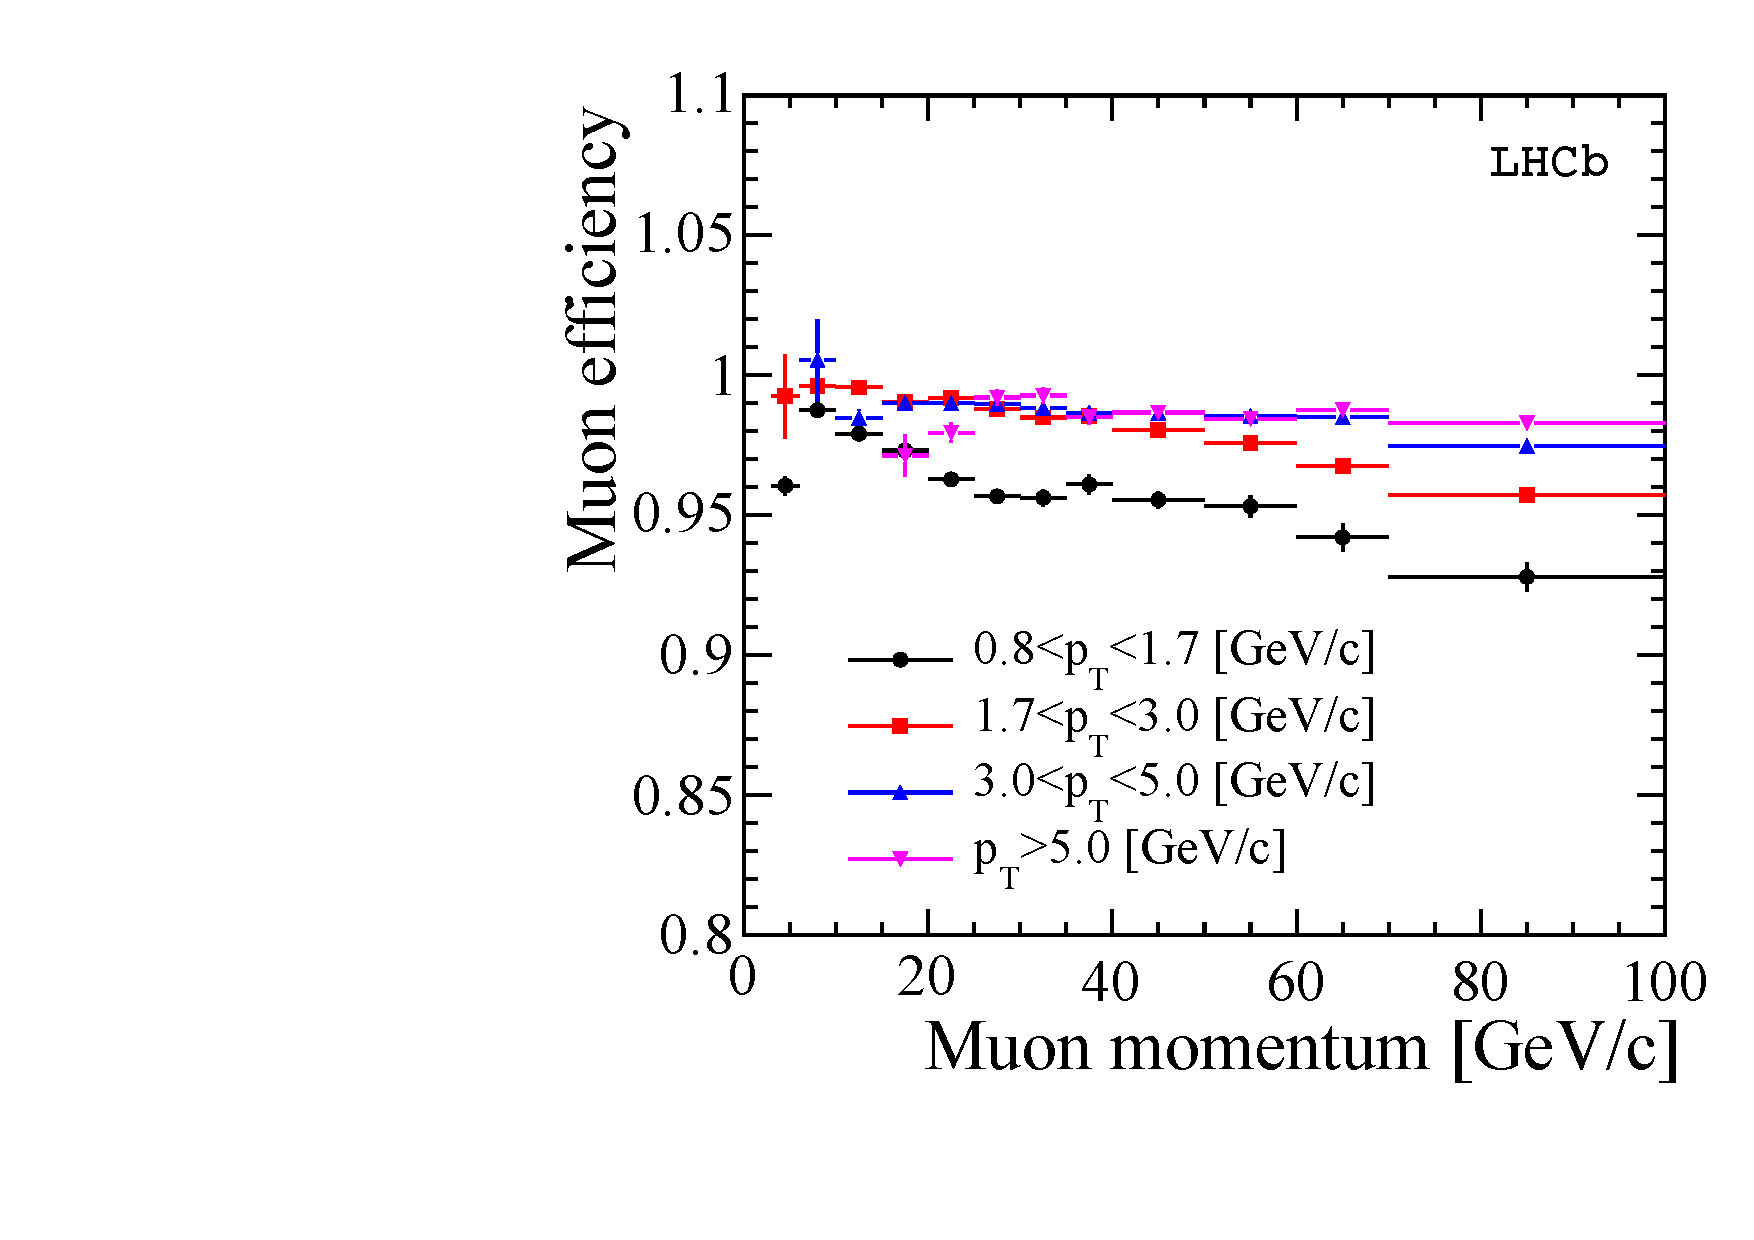
\includegraphics[width=0.49\textwidth]{./Figs/LHC_LHCb/hidef_Fig41topleft.pdf}
  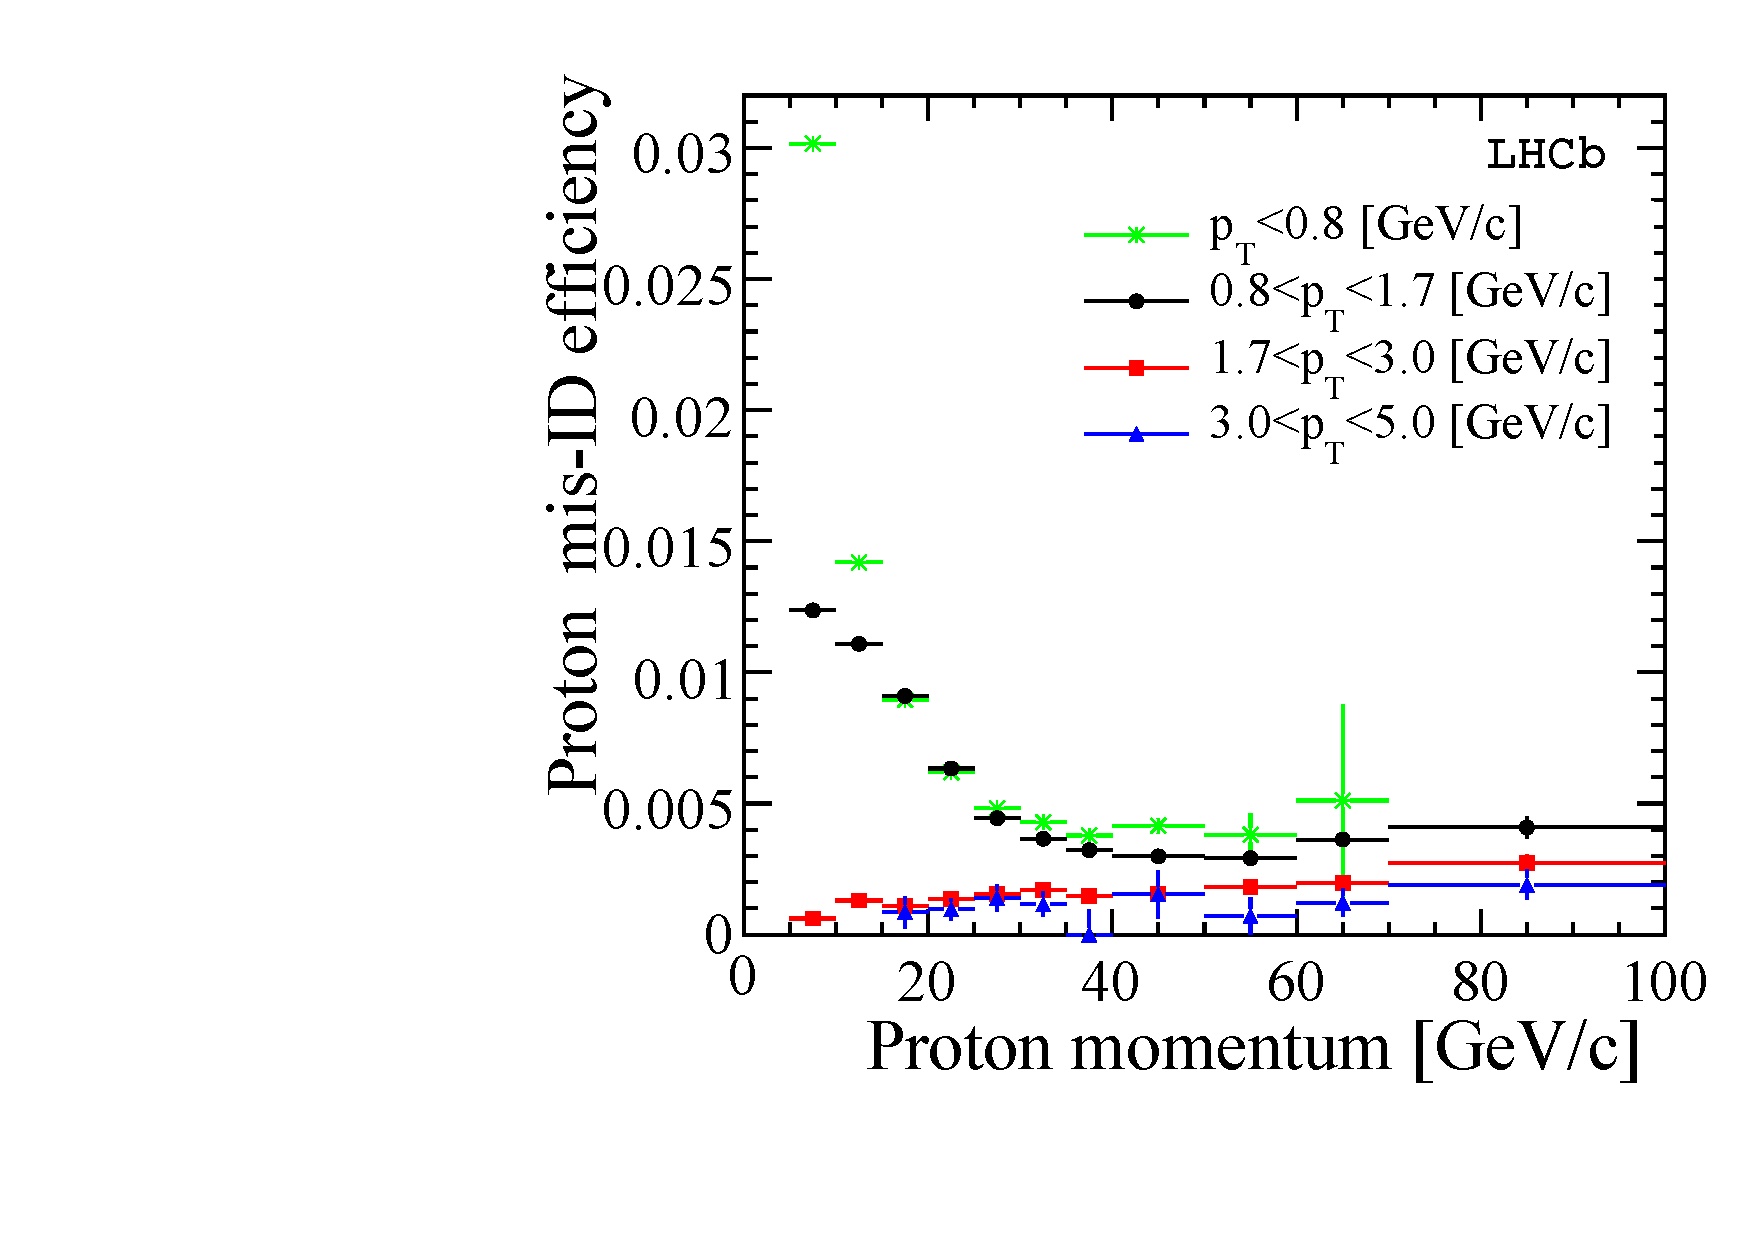
\includegraphics[width=0.49\textwidth]{./Figs/LHC_LHCb/hidef_Fig41topright.pdf}
  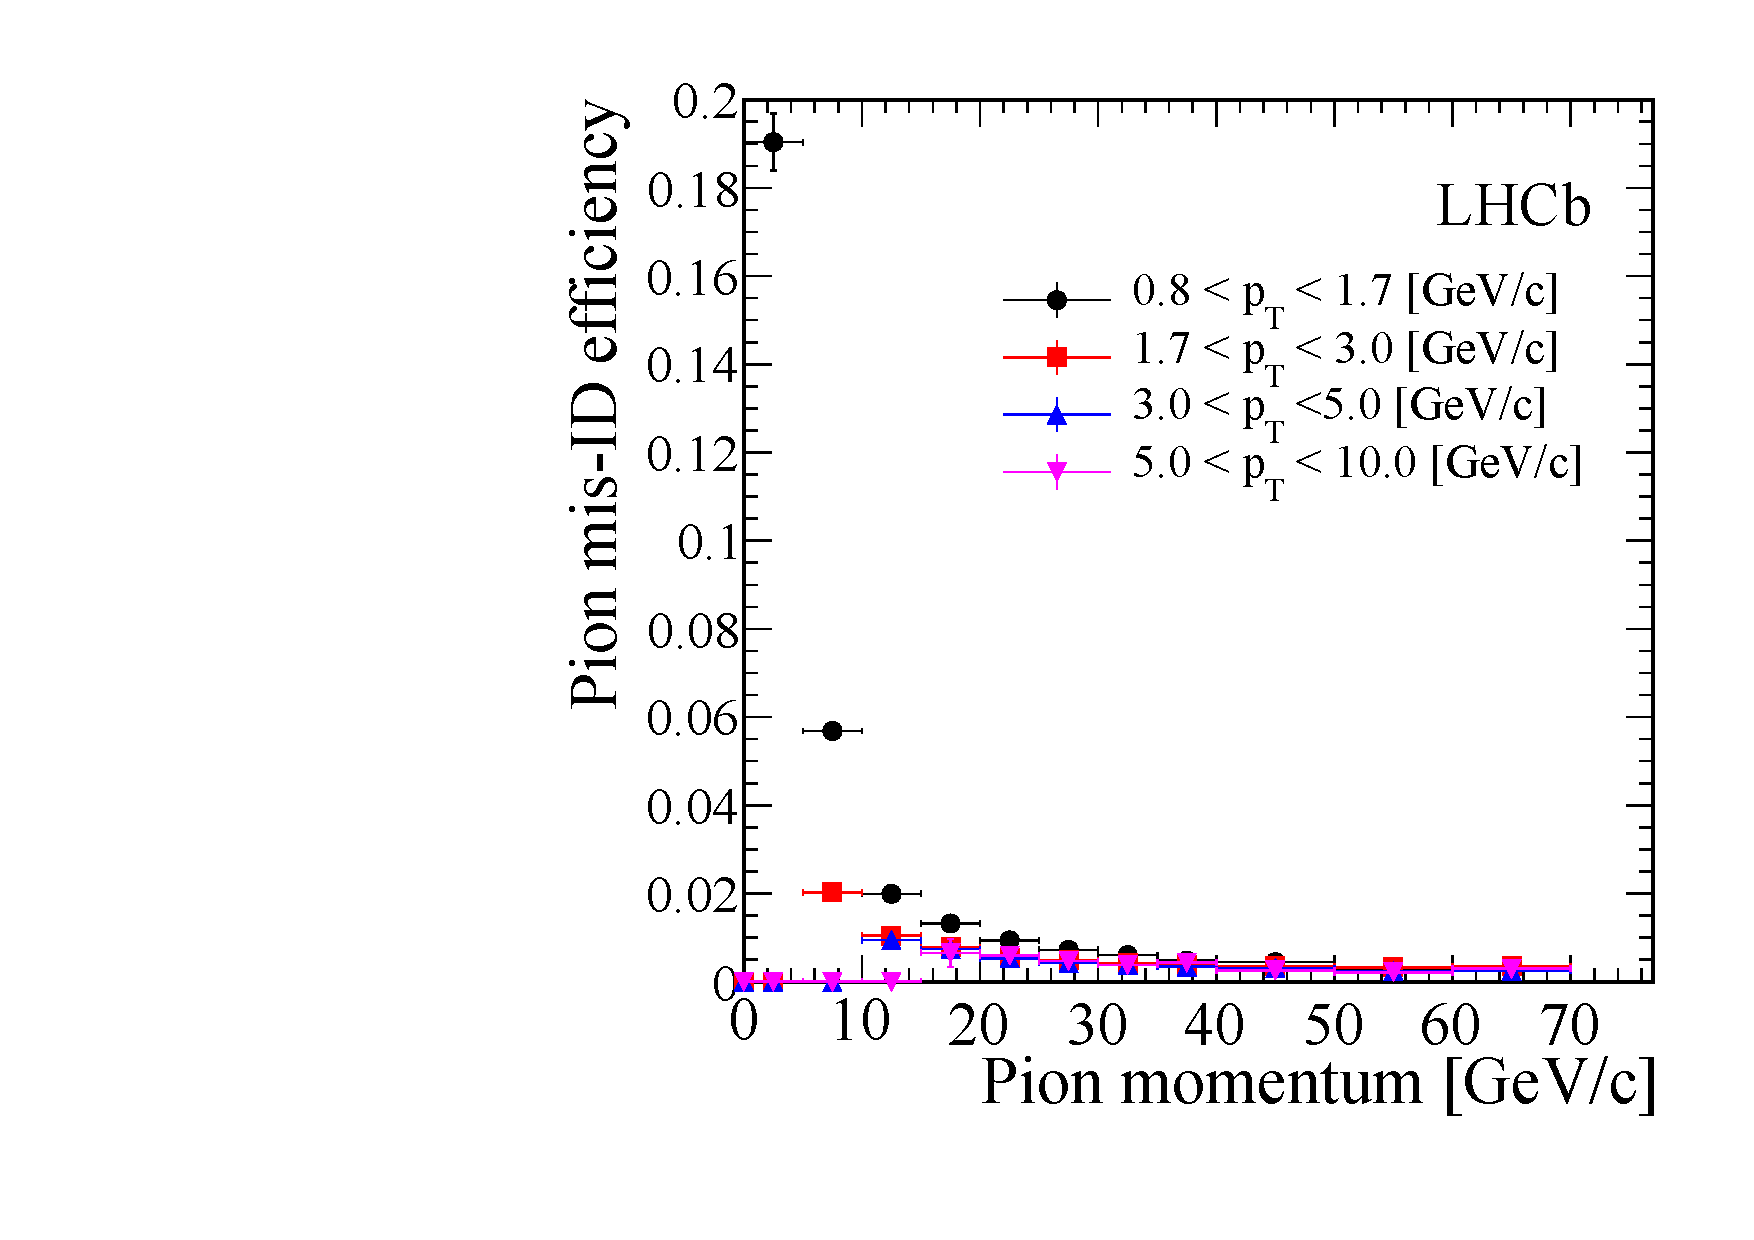
\includegraphics[width=0.49\textwidth]{./Figs/LHC_LHCb/hidef_Fig41bottomleft.pdf}
  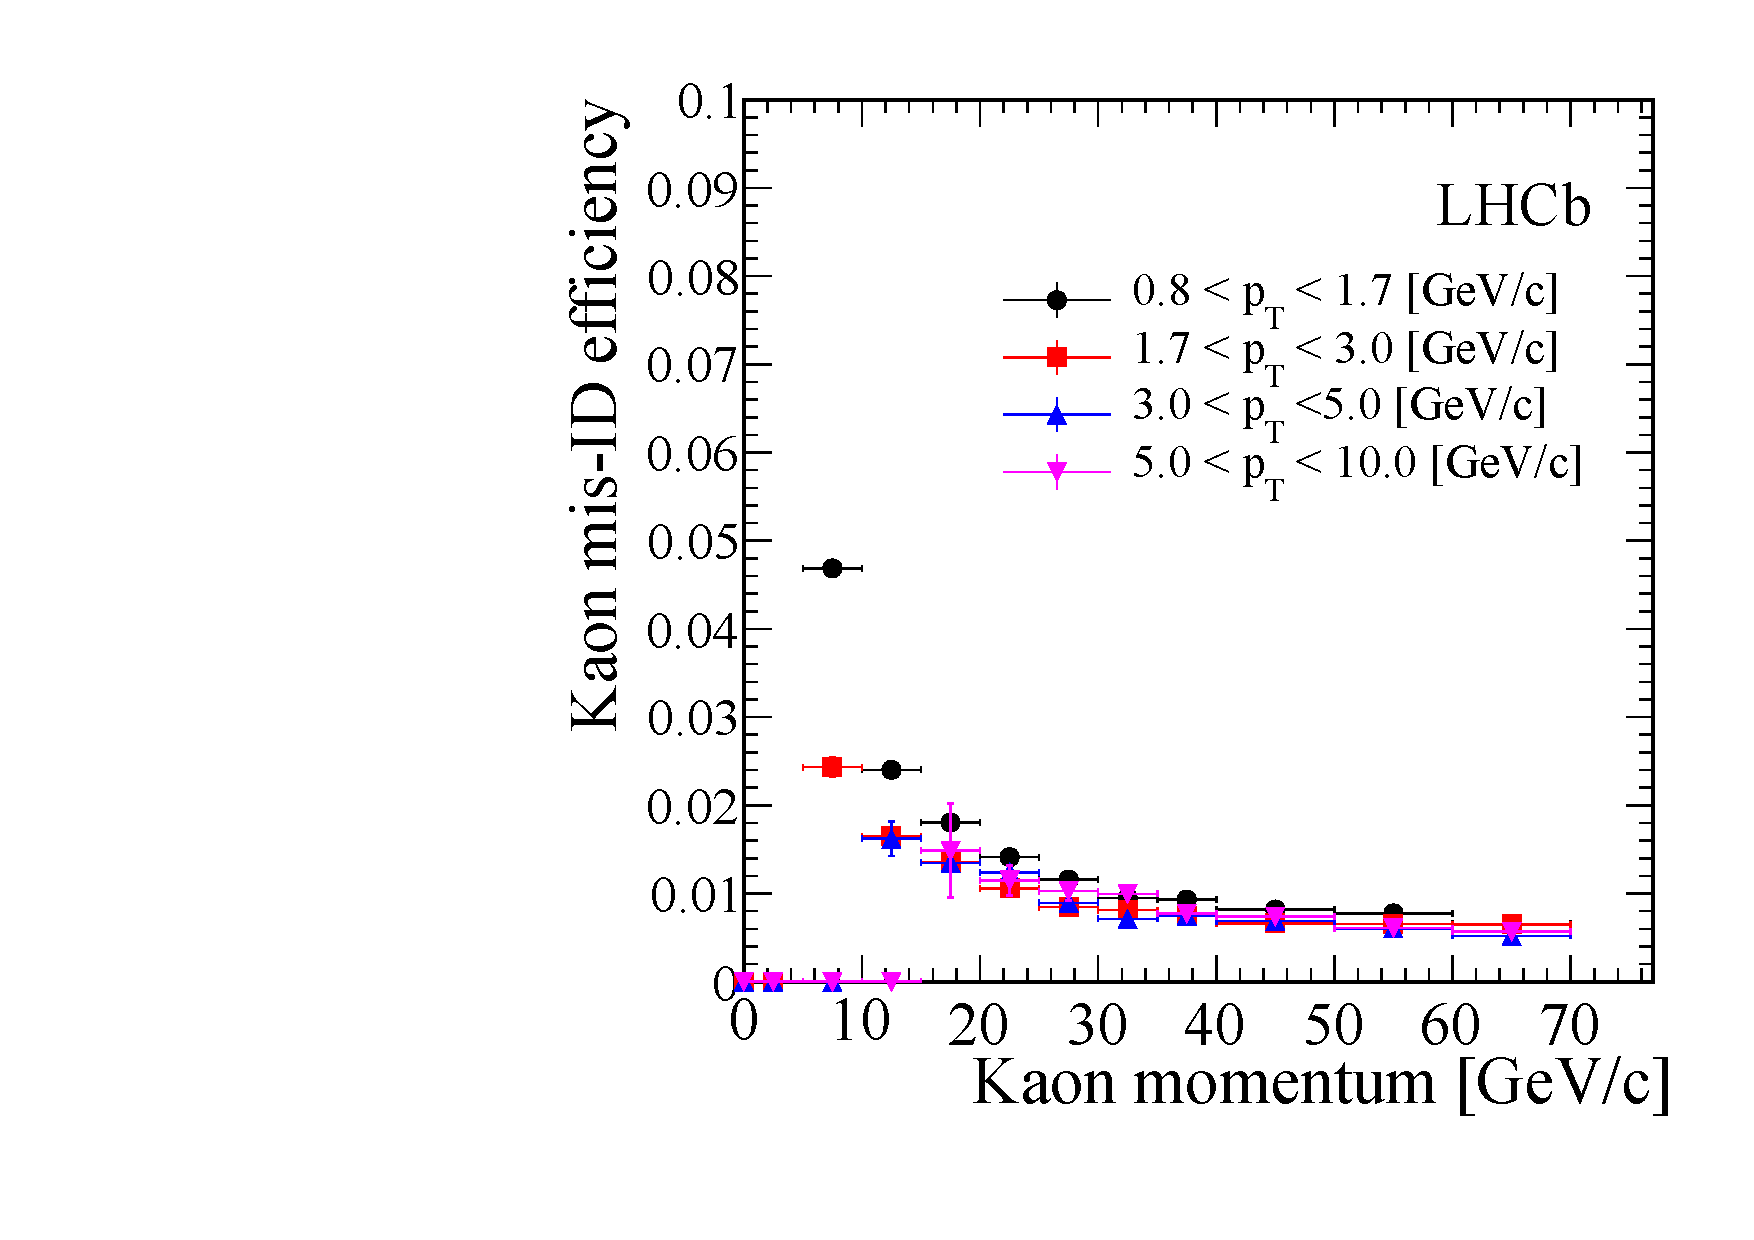
\includegraphics[width=0.49\textwidth]{./Figs/LHC_LHCb/hidef_Fig41bottomright.pdf}
  \caption{Muon efficiency (top left) and mis-identification probabilities for protons (top right), pions (bottom left) and kaons (bottom right) for isMuon criteria \cite{Archilli:2013npa}. }
  \label{fig:isMuon_efficiency}
\end{figure}




The information from all the PID detectors is combined using two different methods to provide global particle identification variables. One method is based on likelihood fits, producing the DLL variables, and the other is based on Neural Networks~\cite{Feindt:2006pm}, producing ProbNN variables. In the first method, likelihood fits are performed in each sub-detector comparing charged particle tracks to different particle hypotheses. The resulting variable is the difference in the log-likelihoods between the track corresponding to a pion and a kaon, proton, muon or electron. The likelihood information from each sub detector is added linearly to form a combined likelihood. 
These variables are called DLL$_{X\pi}$ variables and give a measure of how likely a particle hypothesis of $X$ is compared to that of a pion, where $X$ can be a muon, kaon, proton or electron.

The second approaches uses Neural Networks to combine information from different sub-detectors and to provide a global probability of a track having a particular particle hypothesis. This method takes into account correlations between detector systems and extra detector information that is not considered in the likelihood method. The Neural Networks are trained on simulated inclusive $b$-hadron decays and can be tuned to suit different situations, such as the data taking year. The variables produced by the Neural Networks are called ProbNN variables and ProbNN$X$ corresponds to the probability of a track belonging to a particle hypothesis of $X$ where $X$ is a pion, kaon, proton, muon or electron. 

Figure~\ref{fig:DLL_vs_ProbNN} shows a comparison of the performance of the DLL and ProbNN variables in selecting protons and muons. Although the performance to the two types of variables are quite different, the efficiencies of each variable varies with different kinematic properties of the decay. The most appropriate PID variable type to use depends on the physics analysis it is being used in. 

\begin{figure}[tbp] 
  \centering    
  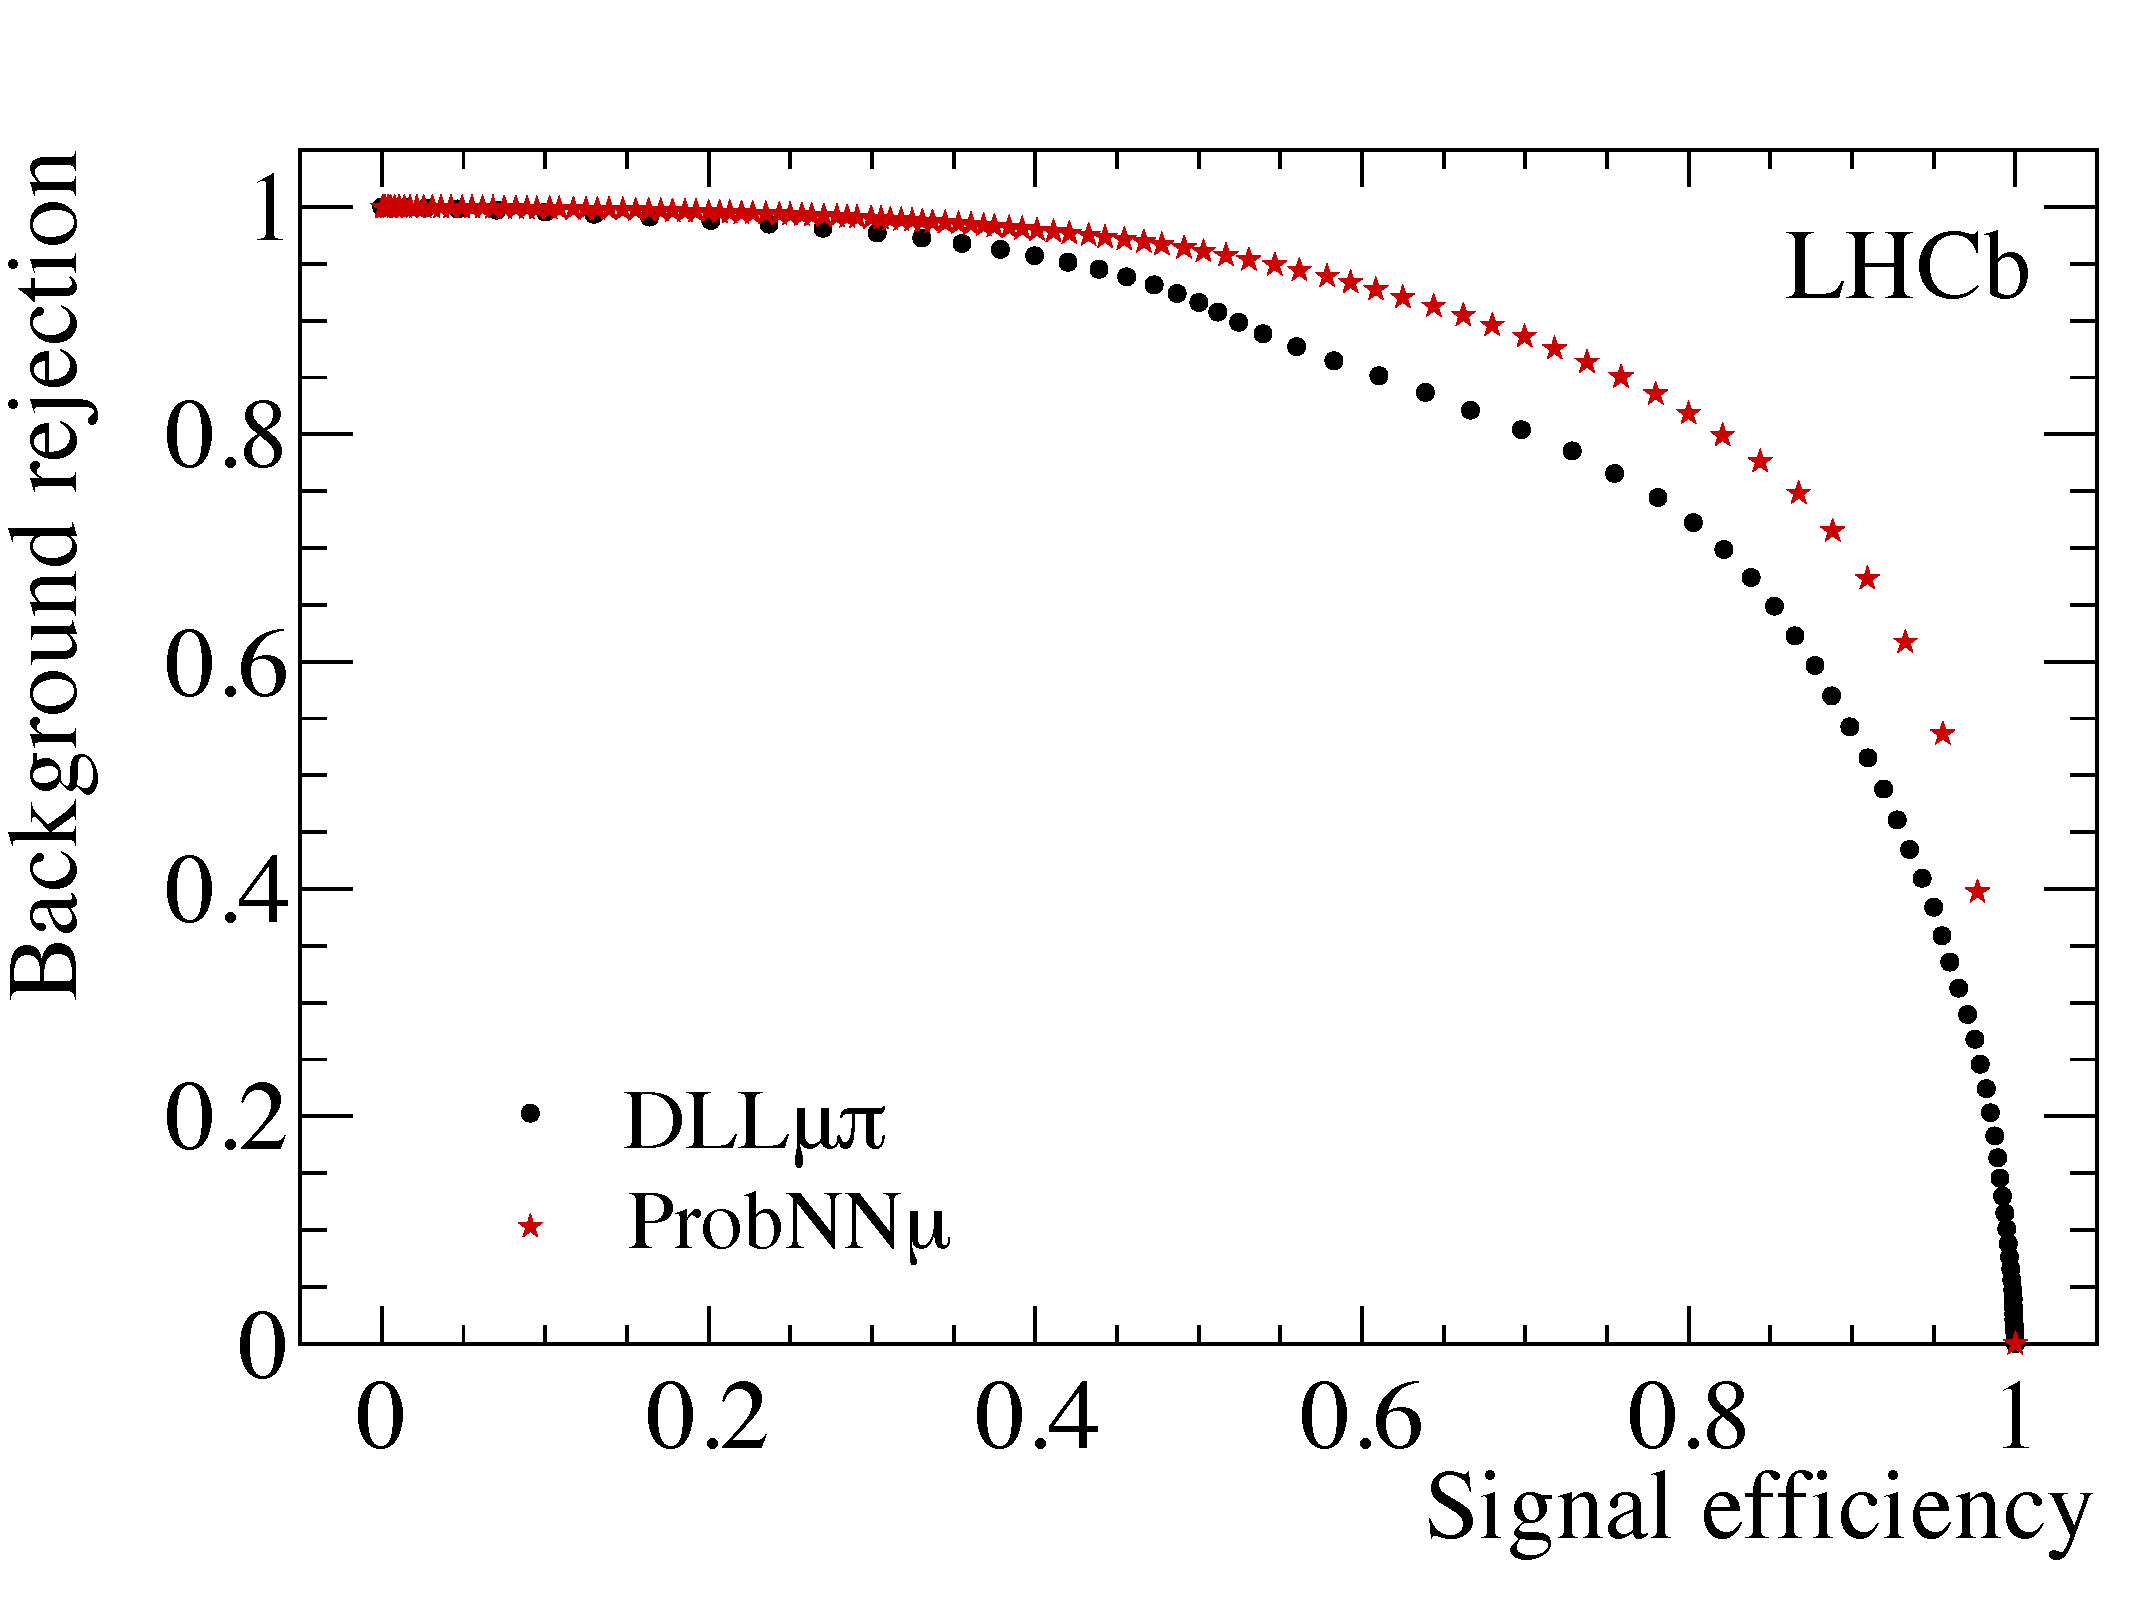
\includegraphics[ width=0.49\textwidth]{./Figs/LHC_LHCb/DLLmu.pdf}%hidef_Fig43left.png}
  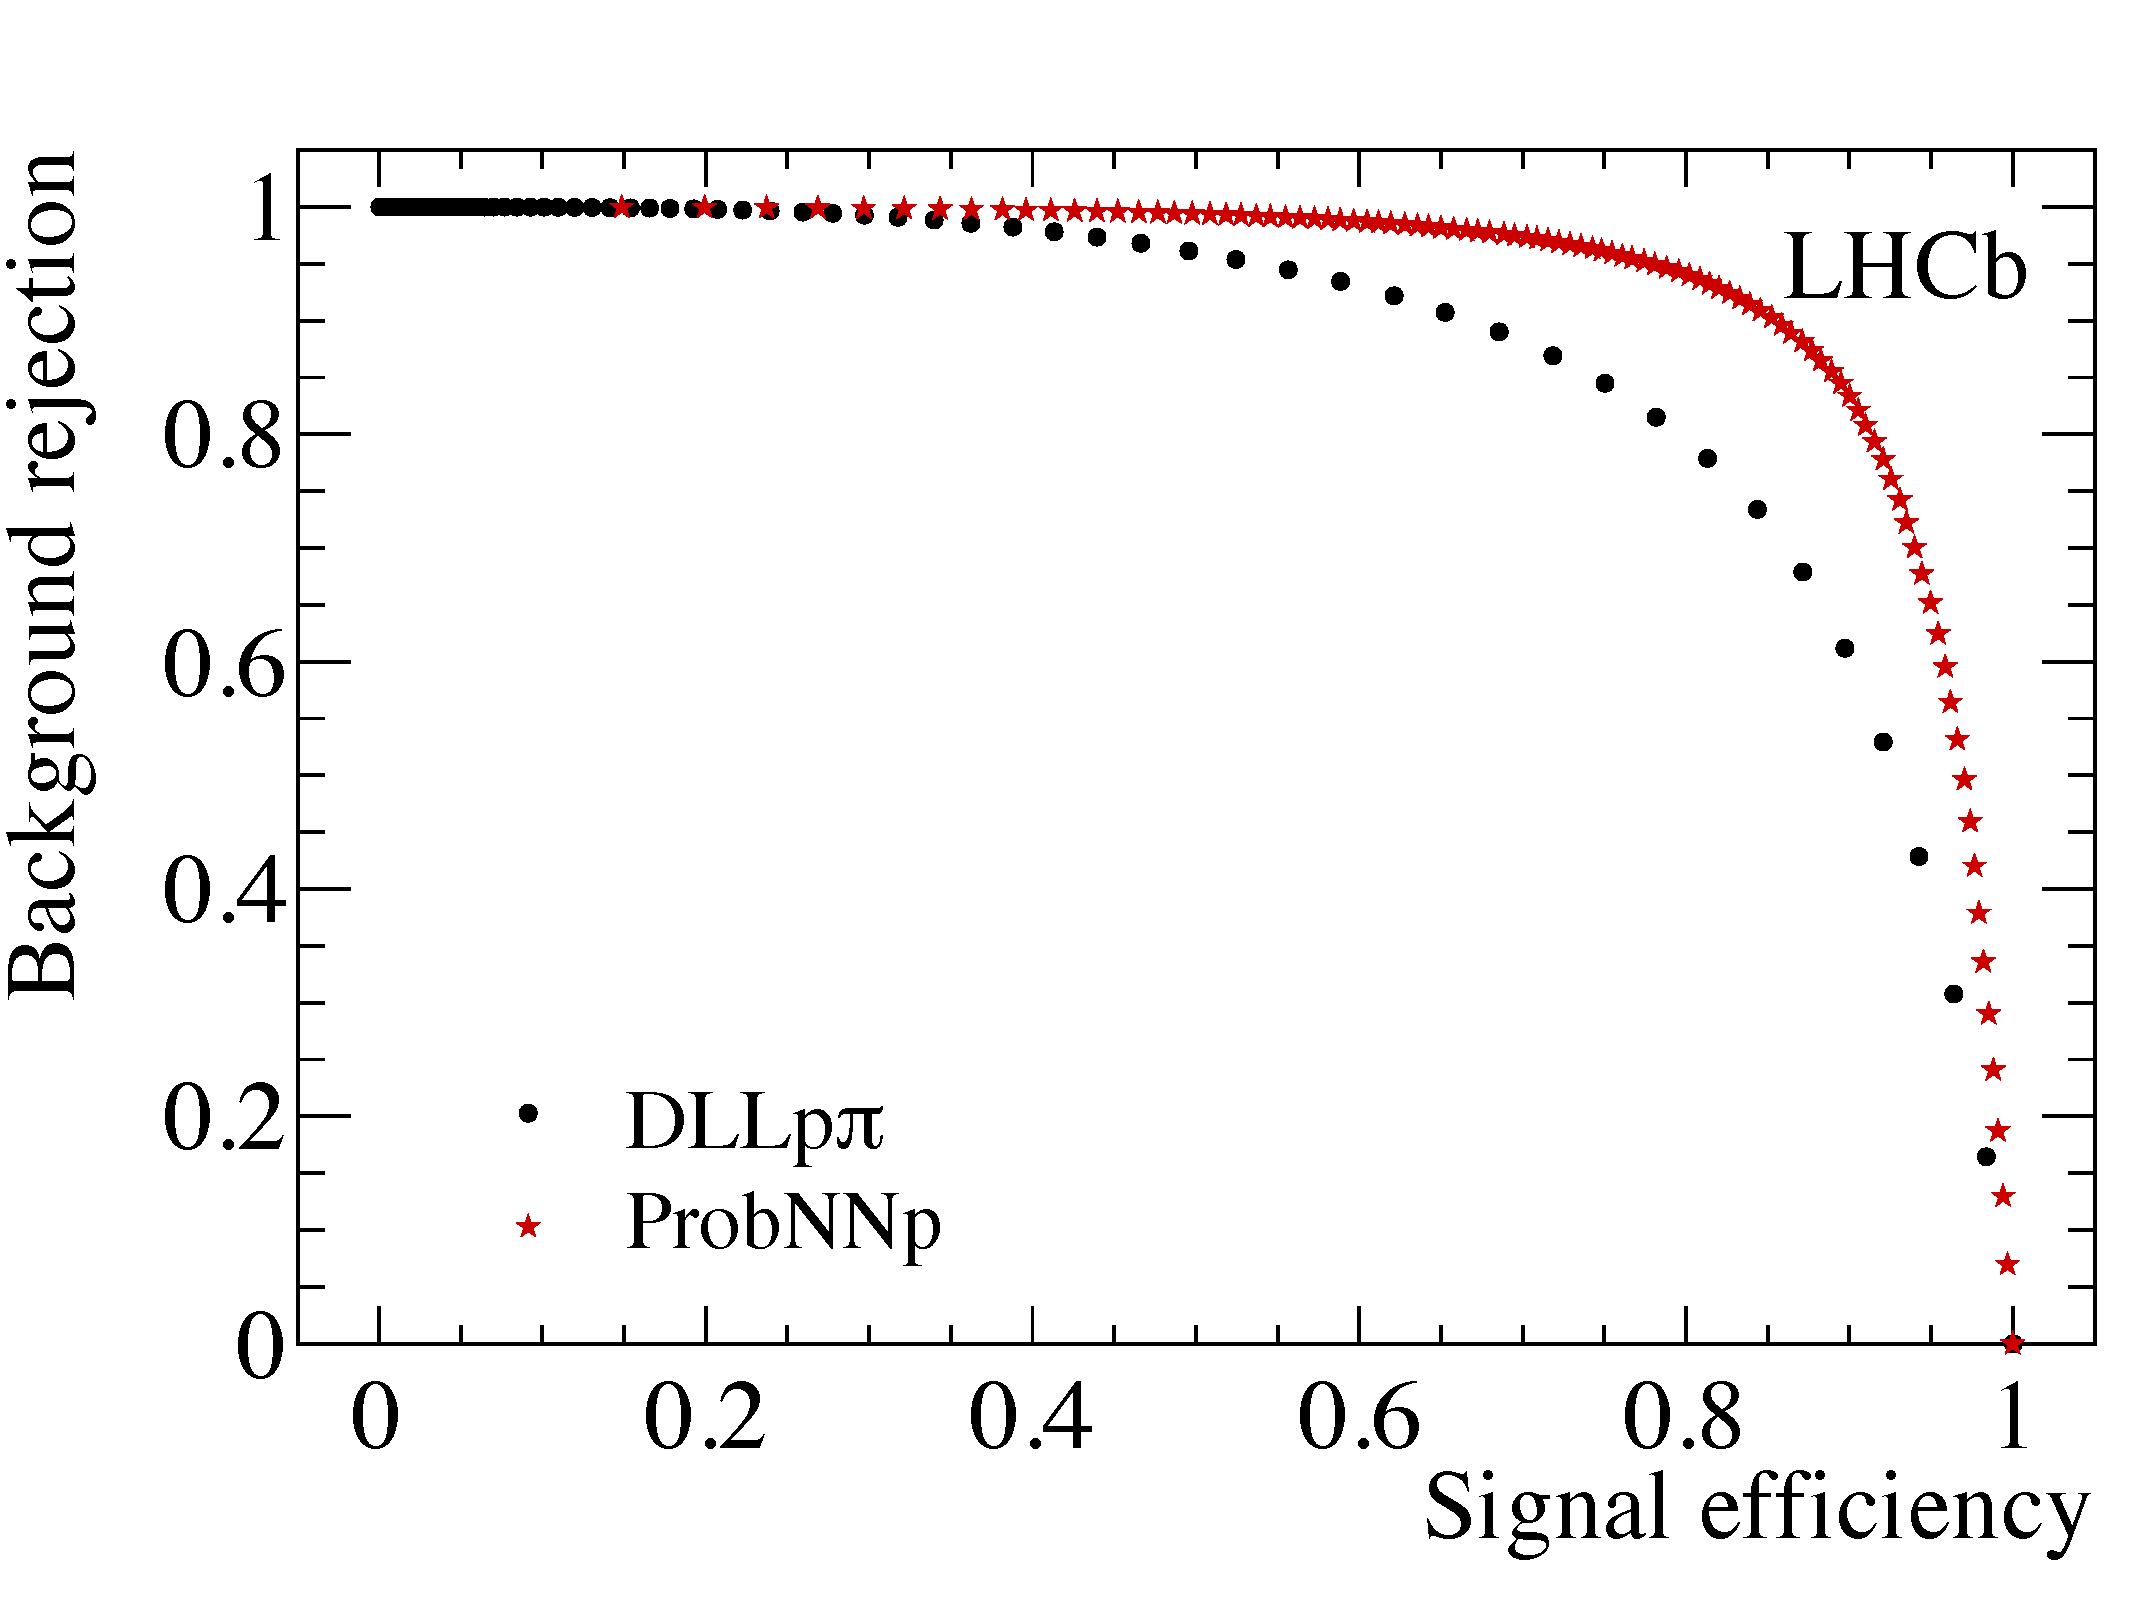
\includegraphics[ width=0.49\textwidth]{./Figs/LHC_LHCb/DLLp.pdf}%hidef_Fig43right.png}
  \caption{Muon (left) and proton (right) signal efficiency vs background rejection for DLL and ProbNN PID variables \cite{Alves:2008zz}.}
  \label{fig:DLL_vs_ProbNN}
\end{figure}

%https://twiki.cern.ch/twiki/bin/view/LHCb/PIDConferencePlots resolution!

\subsection{Trigger}

\label{Trigger}

The LHC was designed to collide protons at a rate of 40 MHz, which is too high for information to be read out by the original design of the LHCb detector\footnote{After the upgrade to the LHCb detector during the second long shut down after 2018, the detector read out will be at 40 MHz}. However, most $pp$ collisions do not produce particles within the detector acceptance that are interesting for the physics processes studied at LHCb. A trigger system~\cite{Alves:2008zz,Aaij:2012me,Albrecht:2013fba} is used to identify $pp$ collisions that contain potentially interesting events, the information from these events is saved and later analysed. The trigger has been designed to select interesting physics events with a high efficiency whilst reducing the event rate to one where information from the full detector can be read out.  There are two levels to the LHCb trigger; the hardware trigger and the software trigger. The hardware trigger is known as the Level-zero (L0) trigger and reduces the 40~MHz collision rate to 1~MHz at which the full detector can be read out. The software trigger is known as the High-Level-Trigger (HLT) and has two stages that run on the output of the L0 further reducing the event rate by utilising information for all the detector sub-systems. Each level of the trigger is composed of trigger `lines'; these lines are made up of reconstruction and selection algorithms and either accept or reject each event. Only events that are accepted by a trigger line at both the L0 and HLT are available for use in physics analyses. 
During the long shut down between Run~1 and Run~2 of the LHC significant changes were made to the reconstruction of particle decays used to make decisions within the HLT. Diagrams of the trigger system used in 2012 and 2015 are shown in Figure~\ref{fig:trigger_diag} and are good illustrations of trigger systems used throughout Run 1 and Run 2, respectively.


\begin{figure}[tbp] 
  \centering    
  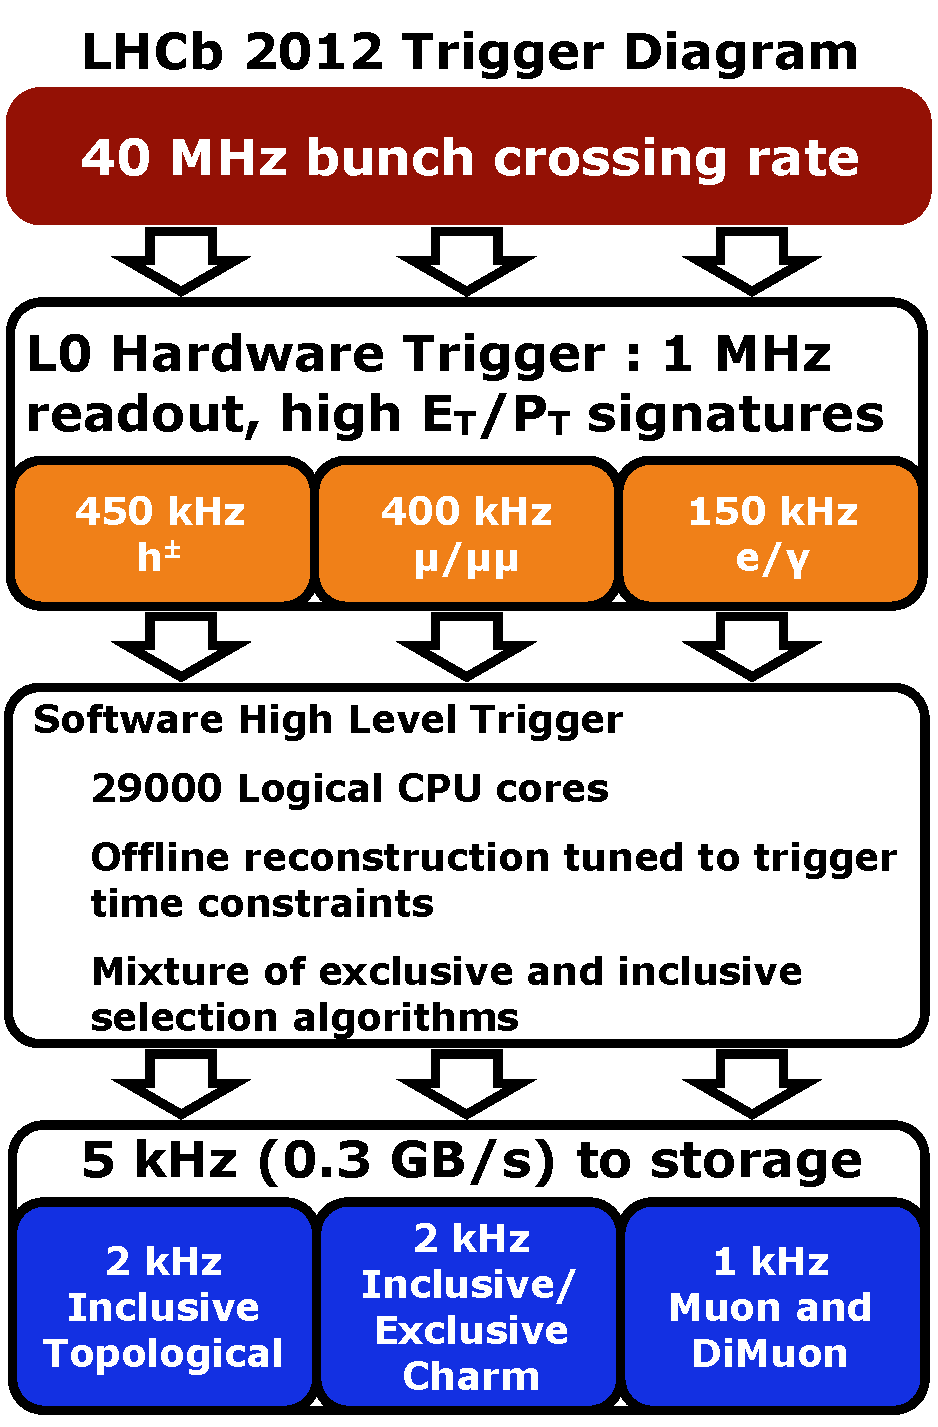
\includegraphics[ width=0.49\textwidth]{./Figs/LHC_LHCb/LHCb_Trigger_RunI_May2015.pdf}
  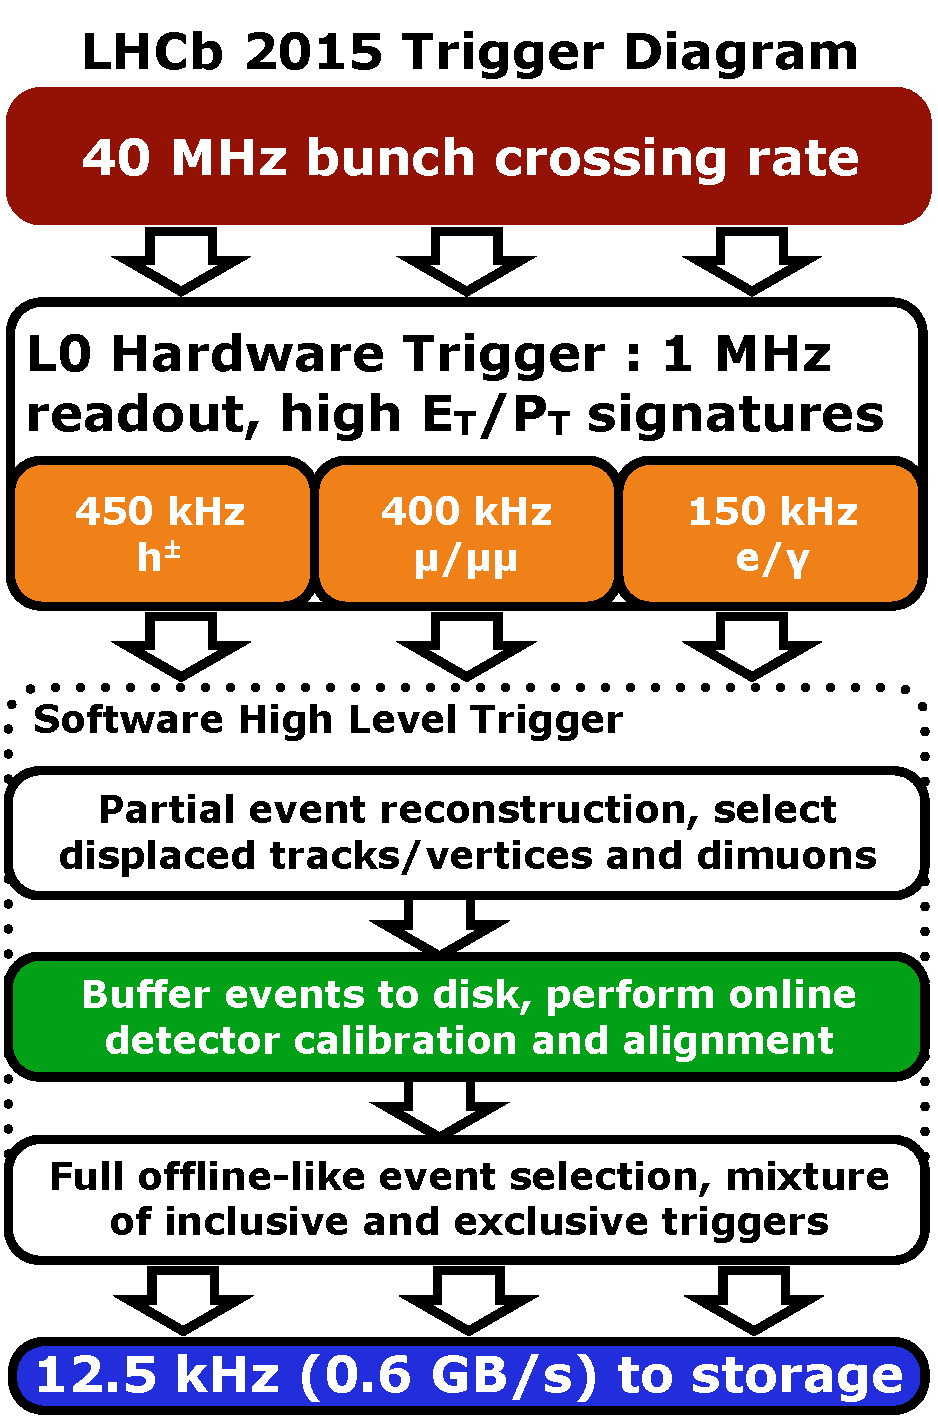
\includegraphics[ width=0.49\textwidth]{./Figs/LHC_LHCb/LHCb_Trigger_RunII_May2015.pdf}

  \caption{Diagrams of the trigger systems used in 2012 (left) and 2015 (right). Source: LHCb.}
  \label{fig:trigger_diag}
\end{figure}

\subsubsection{L0 trigger}
\label{L0}


The L0 trigger runs synchronously to the LHC bunch crossing. Its purpose is to reduce the event rate to 1~MHz, at which point information from the full detector can be read out. The L0 is limited to use information from the detector that can be read at the same rate as the LHC collision rate.
Therefore the L0 uses information from only the VELO, calorimeters and the muon stations to make decisions about the relevance of each event.%; the VELO, calorimeters and the muon stations. 


%The pileup veto stations in the VELO are used in L0 pileup trigger lines, these lines identity the number of collisions in an event and are predominately used for luminosity measurements~\cite{Aaij:2011er}.



The heavy masses of \bhadrons means that their decays are characterised by the production of daughter particles with large transverse momentum ($p_{T}$) and transverse energy ($E_{T}$).
The L0 trigger is designed to identify high $p_{T}$ and $E_{T}$ hadrons, electrons, photons and muons produced in events. Information from the PS, SPD, ECAL and HCAL is used to identify electrons, photons and hadrons in each event. Events are then accepted by the trigger lines if there is an electron, photon or hadron with $E_{T}$ above a threshold value, where the $E_{T}$ thresholds are different for each particle type. % provided the event multiplicity is not too high. The $E_{T}$ thresholds are different for each particle type. 
In a similar way to the calorimeters, the muon stations are used to identify muons with high $p_{T}$ for trigger lines. There are two L0 trigger lines for muons that accept events based on muon $p_{T}$ if either a single muon has a $p_{T}$ above a threshold value or if the two muon combination $\sqrt{p_{T1} \times p_{T2}}$ is above a threshold value.

An additional requirement is placed on events before they can be accepted by any L0 trigger line, this requirement is based on the number of tracks present in an event.
Events containing a large number of tracks, high multiplicity events, take a long time to reconstruct and process in the HLT, therefore it is not efficient to save these events.
The multiplicity is measured by the number of hits in the SPD detector (nSPD) and only events with nSPD lower than a specified value can pass an L0 trigger line.
%The other L0 trigger lines are based on the kinematic properties of \bhadron decays. The heavy masses of \bhadrons means that their decays are characterised by the production of daughter particles with large transverse momentum ($p_{T}$) and transverse energy ($E_{T}$).
%The calorimeters are used to identify events that conating electrons, photons and hadrons with high $E_{T}$. 
%The calorimeters are used in trigger lines that select events containing high $E_{T}$ electrons, photons or hadrons. Information from the PS, SPD, ECAL and HCAL is used to identify electrons, photons and hadrons in each event. Events are then accepted by the trigger lines if there is an electron, photon or hadron with $E_{T}$ above a threshold value provided the event multiplicity is not too high. The $E_{T}$ thresholds are different for each particle type. Events with high multiplicity take a long time to reconstruct and process in the HLT, therefore it is not efficiency to keep these events. The multiplicity is measured by the number of hits in the SPD detector (nSPD), only events with nSPD lower than a specified value can pass an L0 trigger line. 
%In a similar way to the calorimeters, the muon stations are used to identify muons with high $p_{T}$ for trigger lines. There are two L0 trigger lines for muons that accept events based on muon $p_{T}$ if either a single muon has a $p_{T}$ above a threshold value or if the two muons $\sqrt{p_{T1} \times p_{T2}}$ above a threshold value, provided the event multiplicity is not too high. %The L0 muon trigger lines are most important to select \bsmumu candidates. The efficiencies for these 2 lines are show in Figure X, most events are triggered by the L0Muon but some are added by the L0Dimuon lines. 
The $E_{T}$ and $p_{T}$ thresholds and the event multiplicity limit for the L0 trigger lines vary for each year of data taking depending on the bandwidth available for the trigger. % and are shown in table X. 

Finally, there is one other type L0 trigger line that is not used to identify events containing interesting physics processes. The pileup veto stations in the VELO are used in L0 pileup trigger line, these lines identify the number of collisions in an event and are predominately used for luminosity measurements~\cite{Aaij:2011er}.

\subsubsection{HLT trigger}
\label{HLT}

Events that are accepted by the L0 trigger lines are moved to a farm of multiprocessor computing nodes, called the Event Filter Farm, where the HLT is run. The HLT is a software trigger that is split into two levels that are run successively. 

The HLT1 is the first level of the HLT. It runs on the output of the L0 checking the decisions and reducing the event rate. % from 1 MHz for processing in the HLT2. 
The HLT1 trigger lines are composed of generic selection criteria, making decisions that confirm those made in the L0 about particular particle types and also identify generic types of particle decays such as inclusive \bhadron decays. 
The second level of the HLT, the HLT2, runs on the output of the HLT1 trigger and consists of trigger lines designed to select decays relevant to specific physics analyses or particle decay topologies.




During Run~1 time constraints in the HLT1 trigger to process the output of the L0 did not allow for full event reconstruction using all LHCb sub-detectors. Instead the HLT1 ran reconstruction and selection algorithms on information only from the VELO and tracking stations. The reduced output of the HLT1 provided an event rate that was low enough to allow event reconstruction that includes all detector subsystems to be used in the HLT2. However, the reconstruction used in the HLT2 was different to the offline reconstruction that is applied to data before it is analysed. Significant changes were made in the reconstruction used in the HLT between Run 1 and Run 2, the details of the changes made can be found in \cite{Lupton:2230910}. The majority of the changes to the HLT for Run 2 are not relevant for the measurements presented in this dissertation, but the overall change is that the same reconstruction is used in the HLT and the offline reconstruction. 

%These trigger lines are composed of generic selection criteria, making decisions that confirm those made in the L0 about particular particle types and also identify generic types of particle decays such as inclusive \bhadron decays. The second level of the HLT, HLT2, runs on the output of the HLT1 which provides an event rate that is low enough to allow event reconstruction that includes all detector subsystems. The trigger lines in the HLT2 are designed to select decays relevant to specific physics analyses or particle decay topologies, this is made possible by detailed information from the reconstruction. 

Just like the L0 trigger, trigger lines in the HLT vary for each year of data taking; both the selection criteria used in the lines and also new trigger lines are introduced. The number of HLT2 lines increases with each year of data taking as understanding of the capabilities of the experiment increases; there were about 100 HTL2 lines in 2011, 200 in 2012, and 450 in 2015. 

%\subsubsection{Trigger decisions}
%\label{trigger_decisions}
%The trigger lines in the L0 and HLT return three different types of decisions that are used to classify events. The choice of which type of trigger decision to use depends on the particular physics analysis and the signal decay of interest, the decisions can either be used line by line or as global decisions taking all lines together. The different decisions are:
%\begin{itemize}
%\item {\bf TOS}, `triggered on signal', tracks and hits that make up signal candidate of a physics analysis are sufficient for the event to pass the trigger line. 
%\item {\bf TIS}, `triggered independant of signal', if the tracks and hits associated with the signal candidate of a physics analysis are removed from the event, other tracks and hits would still cause the event to pass the trigger line.
%\item {\bf Dec}, refers to whether the event was accepted by the trigger line.
%\end{itemize}

\subsection{Software and simulation}
\label{SoftwareSimulation}
%Options instead of referenes, Susan references the realease areas!

The data that is read out of the LHCb experiment needs further processing before it can be analysed to study the SM and search for NP effects. The \textsc{Gaudi} framework~\cite{Mato:1998gfa} is a C++ framework that is the basis for the software applications needed to process data recorded by the LHCb experiment~\cite{Antunes-Nobrega:835156}. This framework ensures the necessary software is available to all users and changes to the software are implemented across all applications, it is suited to the distributed computing system used in LHCb~\cite{Stagni:2012rs}. 


Once events have been accepted by the trigger, the first step in processing the output of the detector is reconstructing events, this is done by the \textsc{Brunel}~\cite{Brunel} application. The reconstruction is applied to events that are accepted by the trigger for both Run 1 and Run 2 data, however the reconstruction used for Run 2 data is the same as that used in the trigger. The \textsc{Brunel} application takes the digitised detector read out, reconstructs hits in the tracking stations to find particle trajectories and momenta, and combines information from the RICH detectors, calorimeters and muon stations to compute PID variables. The output of processing by the \textsc{Brunel} application are stored in `Data Summary Type' (DST) files. 

Next the \textsc{DaVinci} application~\cite{DV} is used to fit the tracks reconstructed in \textsc{Brunel} with primary and secondary vertices. This application assigns particle hypotheses to each track and reconstructs the decay trees of particles in the detector, computing the kinematic properties of decays. The reconstructed output of the trigger is too large to be stored in one place and to be used by all analysts, therefore a `stripping' procedure is used to break up the data into a manageable size for each the different analyses performed on the data. Each analyst designs a set of loose selection requirements, called stripping lines, specific to their decays of interest. The selections are applied centrally to the reconstructed events and are designed to keep as much of the signal relevant to the analysis as possible but reduce the number background events. Only events that pass the selection criteria of a stripping line are available to be used in analyses. The output of this process are smaller DST files, events passing the stripping selections can either be saved with the full event information or with just the tracks related to the signal candidate. The choice depends on the physics process the stripping line is relevant for. The stripping selection is run a limited number of times and is applied separately to data collected in different years. Requirements are imposed on the amount of data each stripping line can retain, typically the output of a line must be less than 0.05$\%$ of the original data set size if the full event information is saved. Each analyst then uses the \textsc{DaVinci} application one last time to produce \textsc{Root}~\cite{Brun:1997pa} files from the output of their stripping lines, these files display the data and properties of particle decays in histograms and are used to analyses the data. %RooFit has citation \cite{Verkerke:2003ir}


As well as data collected by the experiment, simulated data that mirrors what is expected in the experiment is needed to understand the detector performance and for the analysis of the data. There is a set of software applications that are dedicated to the production of Monte Carlo simulated events within the \textsc{Gaudi} framework. Events are generated using the \textsc{Gauss} application~\cite{1742-6596-331-3-032047, Clemencic:2011zza}, which uses \textsc{Pythia}~\cite{Sjostrand:2006za,Sjostrand:2007gs} to model $pp$ collisions and the production of particles, and then the \textsc{Evt}\textsc{Gen} application~\cite{Lange:2001uf} is used to calculate the decay trees and kinematics of these particles. Final state radiation is modelled using \textsc{Photos}~\cite{Golonka:2005pn}. Both \textsc{Pythia} and \textsc{Evt}\textsc{Gen} have been tuned for the production and decay of particles within the LHCb detector. The \textsc{Geant4}~\cite{Agostinelli:2002hh,Allison:2006ve} toolkit is used to model the interaction of particles as they travel through the LHCb sub-detectors and the hits made by particles in the detector. In the simulation the type of particles generated and how they decay can be specified so that the simulated events of a particular decay can be generated. The \textsc{Boole} application~\cite{boole} then produces the digitised detector read out based on the information from \textsc{Geant4} that mimics the detector read out when data is recorded. The output of \textsc{Boole} encompasses the detector response to the different hits, the electronic read out and the L0 hardware trigger, as well as including additional hits from event spillover and LHC backgrounds. The digitised response of the detector is then processed by \textsc{Brunel} and \textsc{DaVinci} in the same way as the real data to produce the \textsc{Root} files. % used in physics analyses. %RooFit has citation \cite{Verkerke:2003ir}

The LHCb software framework is set up so that it can be used on the Worldwide LHC Computing Grid~\cite{Bird:2011zz, WWCG}, the Grid is made up of computers across the world that each store part for the LHCb data set and simulation data. Despite the stripping process the data produced at LHCb is too large to be stored in one place. The \textsc{Dirac}~\cite{Paterson:1397926} system manages grid sites and the \textsc{Ganga}~\cite{Ganga, Ganga2} project allows the submission analysis code to different grid sites. The grid enables analysts to process and study the large amounts of data produced by LHCb without having to store the data where the analyst is. 





\section{Summary}
\label{LHCb_data}
%Need to find some references for the future projections I suppose. 
%The LHCb experiment is one of 7 experiments that studies the products of $pp$ collisions created by the LHC. 

%The data taking periods of the LHC and the integrated luminoscity collect by the LHCb experiment are described in Section~\ref{}. 

The data collected so far by the LHCb experiment during $pp$ collisions is summarised in Figure~\ref{fig:LHCb_lumi}. The physics analyses described in this dissertation use an integrated luminosity of 4.4~\fb that consists of data recorded during 2011, 2012 and 2015 and up until September of 2016. The break down of the integrated luminosities for each year of data used in this dissertation are given in Table~\ref{tab:Runs2}. The total integrated luminosity of Run~2 is currently less that the total from Run~1. However the production cross section for \bhadrons approximately doubled with the increase in centre-of-mass energy between Run~1 and Run~2, therefore Run~2 data will already contain a comparable number of \bhadron decays as Run~1 data. 


%The expected end of Run~2 is 2018 by which time LHCb is expected to have recorded 5~\fb luminosity during the Run. Run~2 will be followed by a second long shut down period (LS2) in which LHCb shall be upgraded ready to record proton collisions at 14~\tev during Run~3. This run of data taking is expected to be from 2021 - 2024 and by the end of Run~3 LHCb is expected to have collected an integrated luminosity of 23~\fb over all the runs. 

\begin{figure}[tb] 
  \centering    
  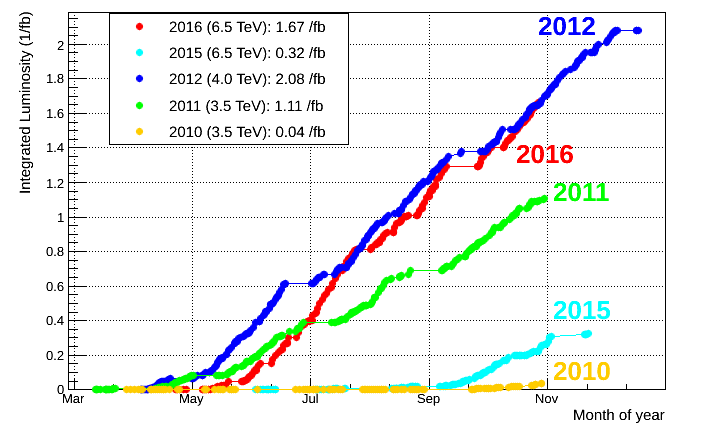
\includegraphics[ width=0.8\textwidth]{./Figs/LHC_LHCb/IntLumiRun1-2.png}
  \caption{Integrated luminosity collected by the LHCb experiment in each year of data taking. Source: LHCb.}
  \label{fig:LHCb_lumi}
\end{figure}

%In Run 1 LHCb ran at an instantaneous luminoscity of 3.5x10^32 cm-2s-1 whereas it was designed to run at 2.0x10^32 cm-2s-1. (Performance paper)

%\begin{figure}[htb] 
%  \centering    
%  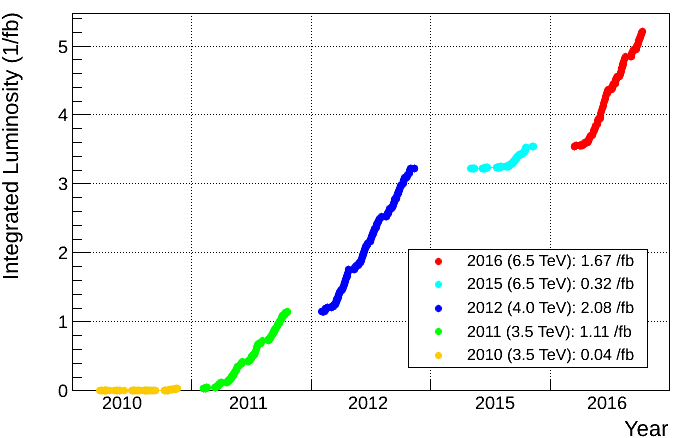
\includegraphics[ width=0.8\textwidth]{./Figs/LHC_LHCb/IntegratedLumiCumul.png}
%  \caption{Cumulative integrated luminosity collected over data taking years at the LHCb experiment. Source: LHCb.}
%  \label{fig:LHCb_lumi_cuml}
%\end{figure}

\begin{table}[bp]
\begin{center}
\begin{tabular}{lccc}
\toprule \toprule
Run & Year & $\sqrt{s}$ / \tev & Integrated luminosity / \fb\\ 
\midrule
 \multirow{2}{*}{Run 1}   & 2011 & 7                             &  1.11 \\
    & 2012 & 8                         &  2.08 \\ 
\midrule
\multirow{2}{*}{Run 2}    & 2015 & 13           & 0.32\\
    & 2016 & 13                                & 1.10     \\ \bottomrule \bottomrule

\end{tabular}
\vspace{0.7cm}
\caption{Integrated luminosity of data collected by the LHCb experiment during $pp$ collisions used in the analyses documented in Chapters~\ref{sec:BFanalysis} and~\ref{sec:lifetimemeasurement}.}
\label{tab:Runs2}
\end{center}
\vspace{-1.0cm}
\end{table}
